% !Mode:: "TeX:UTF-8"
%!TEX program  = xelatex

% 正稿：官方模板封面保留队伍信息；匿名检查从第二页摘要开始。
\documentclass[bwprint]{gmcmthesis}

\hypersetup{hidelinks}
\usepackage[framemethod=TikZ]{mdframed}
\usetikzlibrary{arrows.meta,fit,backgrounds}

\usepackage{subfig}
\usepackage{placeins}
\usepackage{needspace}
\usepackage{siunitx}
\usepackage{chngcntr}
% 官方模板在编号中加入章节号，却没有按章节重置计数器。
\counterwithin{table}{section}
\counterwithin{figure}{section}
\counterwithin{equation}{section}

\usepackage{colortbl}
\usepackage{multirow}
\usepackage{tabularray}
\definecolor{color1}{rgb}{0.78,0.88,0.99}
\definecolor{color2}{rgb}{0.36,0.62,0.84}
\definecolor{color3}{rgb}{0.88,0.92,0.96}
\definecolor{color4}{rgb}{0.96,0.97,0.98}

% 算法
\usepackage[noend]{algpseudocode}
\usepackage{algorithmicx,algorithm}
\floatname{algorithm}{算法}
\renewcommand{\algorithmicrequire}{\textbf{输入:}}
\renewcommand{\algorithmicensure}{\textbf{输出:}}
\algnewcommand{\AlgDescription}{\item[\textbf{说明:}]}

\newcommand{\red}[1]{\textcolor{red}{#1}}
\newcommand{\blue}[1]{\textcolor{blue}{#1}}

% 表格：定宽列自动换行并水平居中；表格内容统一字号。
\newcolumntype{C}[1]{>{\centering\arraybackslash}p{#1}}
\newcolumntype{Y}{>{\centering\arraybackslash}X}
\AtBeginEnvironment{table}{\normalsize\songti}
\AtBeginEnvironment{longtable}{\normalsize\songti}
% 参考文献链接沿用正文西文字体，代码字体保持独立。
\AtBeginEnvironment{thebibliography}{\urlstyle{rm}}

% 使用项目内的字体文件，避免 Linux 上回退到 Fandol。
% 正文字体：Windows 宋体（SimSun）；无真粗体，用 AutoFakeBold 做可辨识的加粗。
\setmainfont{Times.TTF}[Path=fonts/,BoldFont=Timesbd.TTF,ItalicFont=Timesi.TTF,BoldItalicFont=Timesbi.TTF]
\setmonofont{MapleMono-NF-CN-PaperSubset-Light.ttf}[Path=fonts/,Scale=0.92]
\setCJKmainfont{SimSun.ttf}[Path=fonts/,AutoFakeBold=4.5,ItalicFont=SimSun.ttf]
\setCJKsansfont{SimHei.ttf}[Path=fonts/,BoldFont=SimHei.ttf]
\setCJKfamilyfont{zhsong}{SimSun.ttf}[Path=fonts/,AutoFakeBold=4.5]
\setCJKfamilyfont{zhhei}{SimHei.ttf}[Path=fonts/,BoldFont=SimHei.ttf]
\setCJKfamilyfont{zhli}{LiSu.ttf}[Path=fonts/]
\renewcommand{\lishu}{\CJKfamily{zhli}}


%===================== 建模论文题目 ======================

\title{\parbox{\linewidth}{\centering 基于词级时序对齐与文本—音视频混合专家模型的\\[-3pt]多模态情感预测与解释方法研究}}
\baominghao{\hspace{6.3em}26105330055} %参赛队号
\schoolname{\hspace{7.0em}中南大学} %学校名称
\membera{\hspace{6.4em}齐鑫瑶} %队员A
\memberb{\hspace{6.4em}赵鑫渝} %队员B
\memberc{\hspace{6.9em}罗洁} %队员C

%=======================================================


% 题名下横线与文字保留适当间距。
\patchcmd{\makenametitle}{\cline{2-2}}{\noalign{\vskip 3pt}\cline{2-2}}{}{\PackageError{paper}{Title spacing patch failed}{}}

\begin{document}

%生成标题
\maketitle
% 摘要跨页时也统一使用底部居中的页码。
\pagestyle{plain}
% 浮动体会重置字号，在表格内容环境中统一设置，封面不受影响。
\AtBeginEnvironment{tabular}{\normalsize\songti}
\AtBeginEnvironment{tabular*}{\normalsize\songti}
\AtBeginEnvironment{tabularx}{\normalsize\songti}

% 小四字号下保留适当行内留白；以下设置在封面之后生效。
\renewcommand{\arraystretch}{1.35}
\setlength{\aboverulesep}{1.2pt}
\setlength{\belowrulesep}{1.2pt}
\setlength{\abovetopsep}{2.0pt}
\setlength{\belowbottomsep}{2.0pt}
% 普通表格和跨页长表统一铺满正文宽度；表题居中。
\setlength{\LTleft}{0pt plus 1fil}
\setlength{\LTright}{0pt plus 1fil}
\captionsetup[table]{format=plain,justification=centering,singlelinecheck=false}

%填写摘要
\begin{abstract}
针对三模态采样尺度不一致、局部连续信息缺失与预测依据难以追溯的问题，
本文基于CMU-MOSEI多模态系列数据，研究词级时序对齐、缺失感知预测与模态贡献解释。

\textbf{针对问题一}，建立\textbf{基于词时间戳与区间交叠的三模态时序对齐模型}。
以冻结BERT、短窗声学与面部特征提取得到768维、17维和52维表示，结合音文核查与局部边界筛查，
按词时间区间汇聚音视频特征。\textbf{全部100条样本均生成特征表示}，保留原生序列、官方词位置及有效掩码；
\textbf{80条样本中的1533个词建立时间对应}，其中1374个词具有三模态观测。
其余20条按音文不一致、其他语言或无对应语音分类处理，保留原生特征并标记词时间不可用。

\textbf{针对问题二}，使用附件二对齐版的3395条训练样本和728条验证样本，构建
\textbf{文本表征引导的混合专家模型}。文本专家采用冻结BERT表征，音视频专家依据观测掩码编码；
区分结构有效位置与模态观测状态，门控结合专家表示和观测比例融合输出。
通过连续缺失增强、分支监督与音视频向文本表征的辅助重构，联合学习情感极性与强度。
在完整输入的验证集上，三随机种子集成的\textbf{准确率为0.6484}、\textbf{宏平均F1（Macro-F1）为0.6265}，
符号投影后\textbf{MAE为0.5769}、\textbf{Pearson系数为0.6463}。
进一步考察三种模态在首部、中部、尾部缺失20\%或40\%的18种场景，文本缺失影响最大，
其\textbf{六种局部缺失场景的平均Macro-F1为0.5744}；音视频局部缺失的性能波动较小。
完成附件三30条样本的极性与强度预测。

\textbf{针对问题三}，完整枚举8种模态保留组合，计算Shapley贡献，并以连续窗口遮挡定位局部证据，
在预测极性与强度的同时给出\textbf{模态作用程度、主要参考模态与关键证据}。
在728条验证样本上，以20\%窗口选取证据、40\%窗口复核，文本高分窗口的\textbf{平均预测类别概率下降为0.1954}，
高于随机窗口的0.0994和低分窗口的0.0256，表明所选文本片段对模型输出具有较强影响。
对附件四20条样本完成预测与解释，关键文本对应原文；其中7条文本证据具有候选时间区间，
1条视频证据展示邻近画面。

\keywords{多模态情感预测；词级时序对齐；局部模态缺失；混合专家模型；\mbox{Shapley模态贡献}}
\end{abstract}

%目录 不推荐加
\maketoc

\clearpage

% ==================== problem
\section{研究背景及问题重述}
\label{sec:problem}

\subsection{研究背景}

随着自然人机交互、具身智能与智能服务的发展，机器不仅需要识别用户说了什么，
还需要理解其表达中包含的态度和情绪。真实交流中的情感并非由单一信号给出，而是通过
文本语义、语音韵律、面部表情与肢体动作等多种通道协同表达。文本能够反映评价对象、
情感词和上下文语义；语音中的音高、能量、节奏与停顿能够补充说话状态；视频信息则记录
表情、视线和动作变化。对这些线索进行联合分析，有助于减弱单一模态信息不足或表达含糊
带来的误判，因此多模态情感预测已成为情感计算中的重要研究问题。
韩令敏等\citep{han2025review}从特征提取、模态融合和决策分类梳理语音与文本情感识别方法，
将融合方式归纳为特征级、决策级、模型级和多层次融合。

多种模态之间既存在互补，也可能出现不一致。同一句文本在不同语调下可能分别表示赞同、
讽刺或犹豫；积极的词语也可能伴随消极表情，而画面缺少清晰人脸时，视频模态提供的情感
信息又十分有限。若仅依赖文本，容易忽略语气和表情中的补充信息；若简单拼接三类特征，
则难以判断不同模态在当前样本中是否可靠。因而，模型不仅要学习跨模态互补关系，
还要根据每种信息的实际可用程度进行动态取舍。
罗渊贻等\citep{luo2025inconsistency}针对模态间情感语义不一致的问题，结合共性特征、
交叉注意力与模态加权进行融合，为处理相互冲突的情感线索提供了参考。

与规整的实验数据相比，真实视频中的三种信号具有显著的异构性。文本以词或子词组织，
语音以毫秒级短窗采样，视频则由离散帧构成，三者在采样频率、特征维度与时间尺度
上均不相同。词语、声学短窗和视频帧不能直接按照数组下标对应，容器标称时长也未必等于
音视频的实际解码覆盖范围。因此，需要从原始素材出发明确每类特征的定义，并依据真实
时间建立可追溯的对应关系。明确\textbf{多模态特征提取与时序对齐}规则，有助于解释输入表示
的来源及其与原始素材的关系。

实际采集还会出现音轨静音、环境噪声、转写中断、人脸遮挡以及检测失败等情况，使一个或
多个模态在局部连续时间段内不可用。这里的零值可能表示尾部填充、自然未观测或人为遮挡，
三者含义并不相同。若将所有零值都当作真实观测，或仍采用固定融合权重，模型就可能持续
信任已经缺失的信息，造成情感极性和强度预测波动。因此，复杂场景下的模型需要显式区分
结构有效位置与模态观测状态，并具备\textbf{局部模态缺失下的鲁棒预测能力}。

另一方面，情感预测常被直接作为分类或回归结果给出，使用者难以了解模型主要参考了哪种
模态、哪些局部片段真正改变了输出。尤其当文本、语音和视频给出不同线索时，仅展示门控或
注意力权重不足以说明模型行为。为提高结果的可信度，还需要建立\textbf{可量化、可复核的
解释机制}，从模态层面比较三类信息的作用差异，并把局部证据定位回原始文本、语音时段或
视频画面。

基于上述背景，本文以CMU-MOSEI多模态系列数据为研究对象，围绕\textbf{特征构建与时序对齐、
缺失感知预测和分层证据解释}三个层次展开建模。问题一建立原始素材的特征与时间映射，问题二、三基于附件二提供的标准化特征完成预测与解释。

\subsection{相关研究与本文思路}
现有多模态情感建模主要围绕表示融合、时序交互与缺失鲁棒性展开。
王善敏等\citep{wang2025trimodal}从表情、语音、语言及多模态技术出发，梳理了
情感表示、数据资源和识别方法，为三类行为信号的特征组织提供了整体参照。
混合专家模型（Mixture of Experts，MoE）通过门控网络组合多个专家的输出，
其专家分工与输入相关的门控机制可追溯至Jacobs等的研究\citep{jacobs1991moe}。
在融合设计方面，缪裕青等\citep{miao2023gating}通过跨模态门控提取互补信息，
并结合权重与相似约束处理模态贡献差异和情感表达一致性。
魏金龙和邵新慧\citep{wei2024nontext}进一步强化音视频模态，再结合跨模态注意力
与门控融合，以缩小非文本模态与文本的信息差距。
面对不同采样率和未对齐序列，MulT使用定向跨模态注意力学习不同时刻之间的关系\citep{mult2019}。

针对不完整输入，MCT-HFR将局部特征重构与全局表示对齐结合，以缓解随机特征缺失\citep{mcthfr2024}。
王楠等提出随机模态缺失、动态权重调整及教师--学生蒸馏机制\citep{wang2025distill}，
从缺失增强和知识迁移两方面改善模态不完整条件下的表示学习。
陈海丰等\citep{chen2026experts}结合自适应路由和多模态融合专家，依据模态间相关性
与动态权重选择融合策略，并通过共享专家保留共性信息。
这些研究为观测状态驱动的融合与音视频分支强化提供了依据；具体方法仍需在本题统一的
三分类和连续片段缺失设置下验证。

本文依据连续缺失与真实时间可追溯的任务要求，保留结构有效和模态观测两类掩码，
构建包含文本专家和音视频专家的混合专家模型，在两个专家之间进行观测状态驱动的融合，并通过表示辅助约束探索跨模态信息迁移。
实验围绕完整输入、缺失类型、位置和时长展开；解释部分使用固定模型的模态组合与局部遮挡响应，
将融合权重、输出贡献和证据定位分别分析。

\subsection{问题重述}

题目以CMU-MOSEI多模态系列数据为基础，提供附件一原始视频及转写、附件二带标签的标准化特征，
以及附件三局部缺失专项样本和附件四可解释性专项样本。三项任务如下：
\begin{itemize}
 \item \textbf{问题一：三模态特征提取与时序对齐。}
 基于附件一100条原始视频，建立文本、语音、视觉三模态情感特征提取与时序对齐模型，
 明确原始样本处理流程、各模态特征的定义与提取方法，以及跨模态对应规则和实现逻辑。
 生成的特征须覆盖全部样本，记录编号、来源、序列位置、有效长度和填充规则；
 以表格汇总全部100条样本的模态、有效时长、特征维度与对齐粒度，
 并至少展示一个典型样本的三模态对应关系。提交全量特征文件、工具版本、关键参数与复现说明。

 \item \textbf{问题二：局部模态缺失下的鲁棒情感预测。}
 针对一个或多个模态的局部连续时段不可用的情况，构建能够同时输出情感极性和连续强度的
 鲁棒预测模型，说明网络结构、目标函数、训练方案与关键参数。分析缺失模态类型、位置、
 时长及缺失率对预测性能的影响，开展模型比较与消融实验，并给出验证集性能、可视化与错误分析。
 使用固定模型对附件三全部样本推理，以CSV文件提交极性与强度预测。

 \item \textbf{问题三：模态贡献与局部证据解释。}
 面向三模态信息完整但决策依据难以追溯的场景，建立可解释性情感预测模型，
 在输出极性与强度的同时，量化各模态的作用程度、确定主要参考模态并定位关键局部片段。
 关键证据应能对应原始文本、语音时段或视觉关键帧；正文须给出典型样本解释卡、
 局部重要性分布、模态作用对比及验证集评价与错误分析。
 对附件四全部样本输出预测与解释，并以CSV文件提交结果。
\end{itemize}

问题二、三均使用附件二训练集学习参数，在验证集选择结构、超参数和决策阈值，
训练、验证与专项推理保持同一特征版本。极性采用Accuracy和F1评价，
强度采用MAE和Pearson相关系数评价；附件三、四仅用于最终专项推理。
核心代码、模型参数与复现说明见电子附件。

% ==================== analysis
\subsection{总体解题思路}
\label{sec:analysis}

针对三个建模任务，本文按照“\textbf{数据表示—缺失感知预测—预测解释}”的顺序建立
整体方案，并始终保留样本编号、真实时间、结构有效掩码和模态观测掩码。

针对问题一，先为各样本建立共同媒体时间轴，分别提取文本词元、语音短窗和视频显示帧特征。
随后采用\textbf{词时间戳与区间交叠对齐}，依据音文内容核查与局部质量规则，采用符合条件的词时间，
将对应的原生音视频特征汇聚到官方词位置。全部词与原生序列保留，时间不可用及面部缺测分别标记。
通过原生特征与词级表示的计算一致性检验，并结合典型样本分析对齐结果。

针对问题二，采用附件二最多50个位置的对齐序列，只使用训练集拟合参数与标准化统计量，
使用验证集完成模型选择。模型由\textbf{冻结BERT文本专家}、\textbf{掩码感知音视频专家}和\textbf{观测状态驱动的动态门控}组成；在结构有效区间内模拟不同模态、位置和长度的连续缺失，并同步更新
特征和观测掩码。训练时联合优化分类、回归、分支监督与跨模态辅助重构目标，使模型兼顾
\textbf{局部缺失下的极性与强度预测性能}。验证阶段以完整输入为参照，考察缺失模态、位置和比例，
以Accuracy、宏平均 F1（Macro-F1）、Weighted-F1、MAE和Pearson系数综合评价，整模态剔除作为补充压力测试；最终通过三随机
种子集成降低单次训练波动，并用类别结果约束强度符号的一致性。

针对问题三，将文本、语音和视频视为三个合作参与者，枚举全部八种保留组合，计算
精确Shapley模态贡献，比较各模态对当前预测类别概率和情感强度的平均边际作用。
在此基础上，对每种模态的连续位置执行滑动窗口遮挡，确定\textbf{主要参考模态及其关键片段}，
并比较高重要度、随机和低重要度窗口的影响，检验解释对模型行为的忠实性。最后把关键文本
映射回原文，把具备可靠时间证据的候选位置关联到附件四自身的视频；无法确认精确秒数时只
报告特征位置和质量状态，不进行人为线性换算。

问题一自主提取的17维语音和52维视频特征用于回答原始素材如何形成可追溯表示；问题二、三
则使用赛题给定的74维语音与35维视频特征完成监督学习，两类特征分别服务于原始素材对齐与情感预测任务。三问共享
的是\textbf{真实时间、结构有效与实际观测相互分离}的处理原则。问题二、三的模型设计、阈值和版本
选择仅依据附件二训练集与验证集，附件三、四只在方法固定后用于专项推理。
总体技术路线如图\ref{fig:overall-flowchart}所示。

\begin{figure}[htbp]
 \centering
 \resizebox{\linewidth}{!}{% Three parallel tasks; attachment-one features do not feed attachment-two training.
\definecolor{routeblue}{HTML}{394D96}
\definecolor{routeteal}{HTML}{148C84}
\definecolor{routegold}{HTML}{BE913C}
\begin{tikzpicture}[
  x=1cm,y=1cm,>=Latex,
  box/.style={draw=#1!65,line width=.65pt,rounded corners=2pt,
    fill=white,text=black,text width=4.05cm,minimum height=1.60cm,
    align=center,inner sep=5pt,font=\fontsize{8.5}{11.5}\selectfont},
  heading/.style={text=black,font=\fontsize{10}{13}\selectfont\bfseries,align=center},
  flow/.style={->,line width=.8pt,draw=#1!85},
  note/.style={font=\fontsize{8}{10}\selectfont,text=black,align=center}
]
% Soft column backgrounds distinguish tasks without heavy enclosing borders.
\fill[routeblue!4,rounded corners=4pt] (0,0) rectangle (4.8,9.25);
\fill[routeteal!4,rounded corners=4pt] (5.4,0) rectangle (10.2,9.25);
\fill[routegold!5,rounded corners=4pt] (10.8,0) rectangle (15.6,9.25);
\foreach \x/\col in {2.4/routeblue,7.8/routeteal,13.2/routegold}{
  \draw[\col,line width=2pt] (\x-2.1,9.11)--(\x+2.1,9.11);
}
\node[heading] at (2.4,8.70) {问题一\quad 特征构建};
\node[heading] at (7.8,8.70) {问题二\quad 鲁棒预测};
\node[heading] at (13.2,8.70) {问题三\quad 分层解释};

\node[box=routeblue] (a1) at (2.4,7.40) {\textbf{原始素材与时基}\\100条视频与官方转写\\样本编号、音画解码时间};
\node[box=routeblue] (a2) at (2.4,5.30) {\textbf{三模态原生特征}\\BERT文本\quad 短窗声学\\视频面部系数};
\node[box=routeblue] (a3) at (2.4,3.20) {\textbf{词时间戳对齐}\\局部词边界、区间交叠\\观测掩码与来源映射};
\node[box=routeblue,fill=routeblue!9] (a4) at (2.4,1.10) {\textbf{全量特征与汇总}\\100条样本的三模态特征\\时间映射与对齐覆盖};

\node[box=routeteal] (b1) at (7.8,7.40) {\textbf{训练与模型选择}\\附件二对齐版\\训练集拟合、验证集选模};
\node[box=routeteal] (b2) at (7.8,5.30) {\textbf{混合专家训练}\\BERT与音视频编码\\缺失增强、文本表征引导};
\node[box=routeteal] (b3) at (7.8,3.20) {\textbf{MoE预测与集成}\\极性分类、强度回归\\动态门控、三种子集成};
\node[box=routeteal,fill=routeteal!9] (b4) at (7.8,1.10) {\textbf{专项预测结果}\\附件三：30条样本\\情感极性与连续强度};

\node[box=routegold] (c1) at (13.2,7.40) {\textbf{专项样本与解释任务}\\附件四20条样本\\三模态特征与原视频};
\node[box=routegold] (c2) at (13.2,5.30) {\textbf{固定MoE推理}\\沿用集成与决策规则\\预测类别与连续强度};
\node[box=routegold] (c3) at (13.2,3.20) {\textbf{模态贡献与局部证据}\\Shapley与连续窗口遮挡\\验证集宽窗口忠实度复核};
\node[box=routegold,fill=routegold!10] (c4) at (13.2,1.10) {\textbf{预测解释与媒体回溯}\\主要模态、贡献与关键位置\\文本区间与邻近画面};

\foreach \a/\b in {a1/a2,a2/a3,a3/a4}{\draw[flow=routeblue] (\a.south)--(\b.north);}
\foreach \a/\b in {b1/b2,b2/b3,b3/b4}{\draw[flow=routeteal] (\a.south)--(\b.north);}
\foreach \a/\b in {c1/c2,c2/c3,c3/c4}{\draw[flow=routegold] (\a.south)--(\b.north);}
% Short connector in the inter-column gutter carries the fixed ensemble.
\draw[flow=routeteal] (b3.east)--(10.5,3.20)--(10.5,5.30)--(c2.west);
\node[note,rotate=90,fill=white,inner sep=2pt] at (10.5,4.25) {固定模型};

\end{tikzpicture}
}
 \caption{总体技术路线}
 \label{fig:overall-flowchart}
\end{figure}

% ==================== assumptions
\section{模型假设与符号说明}
\label{sec:assumptions}

\subsection{模型假设}

针对三问的建模过程，本文作如下必要假设：

\begin{enumerate}[label=\arabic*.]
 \item 解码后音频帧的累计样本时间与视频帧的显示时间可作为建立音画对应关系的共同
 候选时基。重采样的绝对延迟未经独立标定时，不将音频派生秒数视为确定边界。
 \item 模态是否获得有效观测与该位置是否属于样本有效序列是两种不同状态；结构区间内的
 全零特征可标为未观测，但不由零值推断其具体物理成因。
 \item 在结构有效且已观测的区间内，连续遮挡可作为比较局部模态缺失鲁棒性的实验近似，
 但不要求它覆盖真实环境中的所有缺失机制。
\end{enumerate}

\subsection{定义与符号说明}

本文按照数据表示、情感预测与结果解释三个层次定义主要符号，分别列于表
\ref{tab:symbols-p1}--表\ref{tab:symbols-p3}中。

\begin{table}[htbp]
 \centering
 \caption{样本、时间与特征提取相关符号}
 \label{tab:symbols-p1}
 \begin{tabular*}{\linewidth}{@{\extracolsep{\fill}}cccc@{}}
 \toprule
 符号 & 含义 & 符号 & 含义 \\
 \midrule
 $s$ & 样本编号 & $T_s$ & 样本媒体覆盖终点 \\
 $L_T,L_A,L_V$ & 文本、语音、视频原生长度 & $N_s$ & 官方词数 \\
 $t^{(a)}_{s,i}$ & 第$i$个语音窗候选时间 & $t^{(v)}_{s,j}$ & 第$j$帧显示时间 \\
 $I_i$ & 第$i$个词的时间区间 & $\ell_{ir}$ & 词区间与原生区间交叠长度 \\
 $\boldsymbol h_{s,l}$ & 第$l$个文本词元向量 & $\boldsymbol a_{s,i}$ & 第$i$个17维语音特征 \\
 $\boldsymbol v_{s,j}$ & 第$j$个52维视频特征 & $\omega_{ird}$ & 第$i$词第$d$维的来源$r$权重 \\
 $m^{\rm str}_{s,k}$ & 结构有效掩码 & $m^{(q)}_{s,k}$ & 模态$q$观测掩码 \\
 \bottomrule
 \end{tabular*}
\end{table}

\begin{table}[htbp]
 \centering
 \caption{情感预测与缺失建模相关符号}
 \label{tab:symbols-p2}
 \begin{tabular*}{\linewidth}{@{\extracolsep{\fill}}cccc@{}}
 \toprule
 符号 & 含义 & 符号 & 含义 \\
 \midrule
 $X_s,A_s,V_s$ & 文本、语音、视频输入 & $D^q_{s,t}$ & 人工连续缺失掩码 \\
 $c_s$ & 真实极性类别 & $y_s$ & 真实连续强度 \\
 $\hat{\boldsymbol p}_s$ & 三分类预测概率 & $\hat y_s$ & 预测强度 \\
 $\boldsymbol r_s^x$ & 冻结BERT片段表示 & $\boldsymbol r_s^{av}$ & 音视频专家隐表示 \\
 $g_s$ & 文本专家门控比例 & $\rho_s^q$ & 模态$q$观测比例 \\
 $\mathcal L_{\rm cls}$ & 加权分类损失 & $\mathcal L_{\rm reg}$ & SmoothL1回归损失 \\
 $S$ & 模型选择综合分数 & $r$ & Pearson相关系数 \\
 \bottomrule
 \end{tabular*}
\end{table}

\begin{table}[htbp]
 \centering
 \caption{可解释性分析相关符号}
 \label{tab:symbols-p3}
 \begin{tabular*}{\linewidth}{@{\extracolsep{\fill}}cccc@{}}
 \toprule
 符号 & 含义 & 符号 & 含义 \\
 \midrule
 $M$ & 三模态参与者集合 & $S\subseteq M$ & 保留的模态子集 \\
 $v(S)$ & 子集输入下当前类别概率 & $\phi_q$ & 模态$q$的Shapley贡献 \\
 $I$ & 连续局部窗口 & $d_q(I)$ & 遮挡窗口后的概率下降 \\
 $c^*$ & 完整输入预测类别 & $\boldsymbol x\setminus I$ & 遮挡局部证据后的输入 \\
 \bottomrule
 \end{tabular*}
\end{table}

除特别说明外，上标 $x,a,v$ 分别代表文本、语音、视频，$q$ 表示其中任一模态；
下标 $s,t$ 分别表示样本和时序位置。结构掩码与观测掩码始终分别存储，不使用同一个
符号同时表示尾部填充和局部缺失。

向量和矩阵使用粗体或大写字母，集合使用花体字母，标量使用普通斜体；带帽符号表示模型
预测，横线表示样本均值。问题一用于聚合的时间区间采用左闭右开形式；特征位置范围采用包含首尾位置的整数索引。
概率贡献以当前完整输入的预测类别为目标，强度贡献另行计算，二者不混用。百分比缺失长度
均相对于样本自身结构有效区间或实际观测长度计算，而不是固定的50个填充位置。

% ==================== dataset
\section{数据集介绍与探索性分析}
\label{sec:dataset}

\subsection{数据集组成}

本题数据以CMU-MOSEI多模态系列数据为基础\citep{mosei2018}，包含文本、语音和视频三种信息。附件一保留
原始视频和官方英文转写，用于三模态特征提取与时序对齐；附件二至四提供预提取
特征，其中附件二含监督标签，附件三、四分别用于局部缺失条件下的预测与解释。各附件的样本规模与特征组成见表~\ref{tab:dataset-scale}。

\begin{table}[htbp]
 \centering
 \caption{四组附件的样本规模与主要字段}
 \label{tab:dataset-scale}
 \begin{tabular*}{\linewidth}{@{\extracolsep{\fill}}ccccc@{}}
 \toprule
 数据 & 样本规模 & 文本 & 语音／视频 & 标签 \\
 \midrule
 附件一 & 100条视频 & 官方英文转写 & 原始音轨／视频帧 & 极性与强度 \\
 附件二对齐版 & 3395/728/727 & $50\times768$ & $50\times74$／$50\times35$ & 有 \\
 附件二未对齐版 & 3395/728/727 & $50\times768$ & $500\times74$／$500\times35$ & 有 \\
 附件三 & 30条 & 对齐版含词元序列 & 两个版本均提供 & 无 \\
 附件四 & 20条及视频 & 原文、词元和向量 & 两个版本均提供 & 无 \\
 \bottomrule
 \end{tabular*}
\end{table}

附件二三个划分的样本数分别为3395、728和727。其对齐版文本、语音、视频最多均为
50个位置，维度分别为768、74和35；未对齐版的音视频长度扩展到500，并另给部分长度
字段。附件三对齐版没有现成的768维文本向量，但保留BERT词元编号、句段编号与注意力掩码，可由固定文本编码器
重建；附件三未对齐版只有原文和500位置音视频。考虑训练与专项预测所需输入的一致性，问题二
与问题三最终采用对齐版。

附件一100条视频来自37个视频目录。解码后音频覆盖终点为2.228--29.110~s，视频为
2.236--29.267~s；文本词元数为7--84，平均25.17。全部1932个官方词位置保留，其中1533个取得可用时间。时长按实际解码得到的媒体时间统计。

\subsection{标签分布分析}

附件二极性标签取 $0,1,2$，分别对应负向、中性和正向；强度位于 $[-3,3]$。训练集和验证集中，极性类别均与强度符号一致：负向对应负值，中性对应零，正向对应正值。训练集负向、中性、正向分别为967、758、1670条，占比28.48\%、
22.33\%和49.19\%；验证集分别为206、184、338条，占比28.30\%、25.27\%和46.43\%。

正向样本接近训练集的一半，中性最少，类别分布并不均衡。若只优化总体准确率，模型可能
倾向正向类而忽略中性边界。因此问题二使用训练集类别频数平方根倒数作为交叉熵权重，
并将三类等权的Macro-F1作为主要分类指标，同时报告逐类F1。训练和验证的类别比例较为
接近；该比较仅涉及类别比例。验证集参与模型选择，所报指标属于开发阶段的评价结果。

\subsection{序列长度与掩码分析}

对齐版文本注意力有效长度在3--50之间，训练集均值为24.65；253条训练样本达到50位置，
可能包含触及上限的长文本。所有注意力掩码都是连续有效前缀，首位均为
\texttt{[CLS]}，末有效位均为\texttt{[SEP]}，segment ID均为0。文本768维数组在填充
区间仍可能非零，因此文本长度必须依赖词元注意力掩码，不能用向量零行判断。

训练集结构区间共83672个位置。语音其中76817个位置非零，观测比例91.81\%；视频
72633个位置非零，观测比例86.81\%。相应的结构内零行比例为8.19\%和13.19\%。这些
零行可代表自然缺测或预处理结果，题目没有提供足以区分成因的字段，本文只把它们记作
未观测。位置0和末有效位置的音视频均为零，与对齐版的特殊词元位置相符，更说明结构
有效与模态观测需要分别表示。图~\ref{fig:dataset-overview} 汇总训练集与验证集的
情感极性构成，以及训练集语音、视频在结构有效区间内按非零行统计的观测比例。

\begin{figure}[htbp]
 \centering
 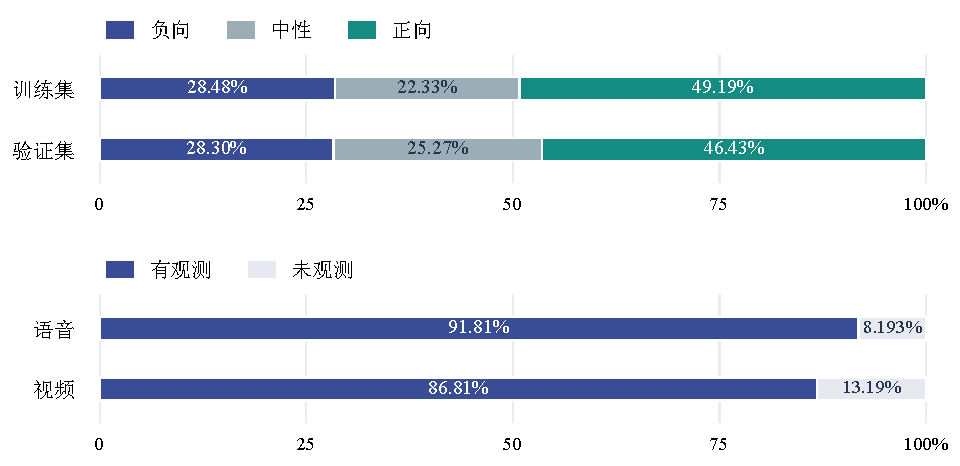
\includegraphics[width=\linewidth]{figures/数据概览.pdf}
 \caption{附件二情感极性构成与模态观测比例}
 \label{fig:dataset-overview}
\end{figure}

\subsection{附件一原始素材特征}

附件一与附件二用途不同，其统计能够直接揭示原始采集中的复杂情况。100条样本共得到
77510个25~ms语音窗和23241个视频显示帧；80条样本中的1533个词取得可用时间，
均有音频窗和视频帧来源，其中1374个取得面部特征。听审确认14条音文内容不一致、
3条其他语言和3条未听到对应语音，分别保留异常记录。

原始素材的可解码性与特征可用性需要分别描述。视频帧存在但未检出人脸时，
仅将面部特征标记为不可用；低能量音轨仍保留音频来源及相应声学特征。
问题一据此设置多层掩码，问题二在赛题提供的特征上采用相同区分，
把结构内零行标为未观测，并在训练时另外生成可控的连续缺失。

\subsection{数据版本比较与最终选择}

未对齐版保留最多500个音视频位置，保留的时序位置更多，但部分视频长度字段与非零位置分布不一致；附件三未对齐版又缺少训练集相同定义的词元和有效长度字段。使用该版本需要明确独立序列长度与跨模态交互规则。
对齐版的三种模态均以50位置组织，附件二训练、验证数据与附件三具有一致的词元输入和音视频特征结构。

因此，附件一保留自主提取的原生时序及词区间映射，用于完成问题一；问题二、三固定使用
附件二至四最多50个位置的对齐序列。两类数据采用一致的掩码原则，音视频特征定义分别说明。
模型与参数确定后，对附件三、四进行专项预测，其结果不参与模型选择。

% ==================== problem1
\section{问题一：三模态特征提取与词级对齐}
\label{sec:problem1}
\subsection{问题分析与总体方案}
文本、语音和视频分别以词元、声学短窗和显示帧组织，三者长度与采样频率不同。
本文建立\textbf{基于词时间戳与区间交叠的三模态时序对齐模型}：
以官方英文文本中的单词为对应单位进行词级对齐，估计其在语音中的起止时间，再汇聚该区间内的语音与视频特征。
每个词使用自身的时间区间，序列长度随官方词数变化。

处理流程为：原视频检查与音视频解码、建立共同媒体时间轴、提取三模态原生特征、
估计并筛查词时间、按交叠区间聚合、输出特征及来源记录。
音文内容核查决定可对齐的范围；逐词质量检查决定哪些时间可以用于聚合。
未获得可用时间的词仍保留其原文、位置和文本向量，原生音视频序列也完整保存。

\subsection{共同媒体时间轴与原生特征}
附件一的37个视频目录共包含100条片段。视频目录编号与片段编号共同确定样本，
并连接官方转写、标签、原视频及特征文件。提取过程不修改官方转写与情感标签。
音视频时间统一换算为媒体秒数：若解码帧显示时间戳为 $p_j$，时基为 $b$，则
\begin{equation}
 t_j=p_jb,\qquad
 A_r=[t_0^{(a)}+n_r/16000,\ t_0^{(a)}+(n_r+400)/16000),
 \label{eq:p1-native-time}
\end{equation}
其中 $t_0^{(a)}$ 为音频起点，$n_r$ 为16 kHz波形中第 $r$ 个声学窗的起始样本索引。
保留音视频原有的相对起点。解码后的两路覆盖范围分别记录，音频重采样的绝对延迟尚未单独标定。

全部100条样本通过帧时间单调性和音频累计样本时间检查，两路首帧时间均为零，
音频帧时间与累计样本时间的最大残差为 $4.990\times10^{-7}$~s。
图~\ref{fig:p1-timebase} 给出视频终点减音频终点的分布，96条的绝对差超过约一个AAC帧时长。
这些差异用于限定各模态的实际覆盖范围。
\begin{figure}[htbp]
 \centering
 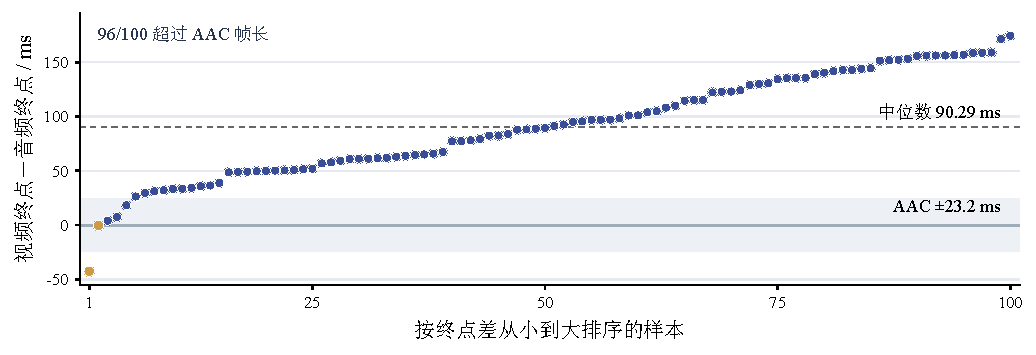
\includegraphics[width=0.98\linewidth]{figures/音画时间基准.pdf}
 \caption{音画解码覆盖终点差分布}
 \label{fig:p1-timebase}
\end{figure}
\subsubsection{文本特征提取}
只使用附件一标签表中的官方英文转写。
冻结的英文 BERT 基础模型（\texttt{bert-base-\allowbreak uncased}）分词器和编码器\citep{bert_acl_online}
产生词元编号、注意力掩码、词到子词索引、内容词元的 $768$ 维末层向量及
\texttt{[CLS]} 向量。编码器不按本题情感标签训练。
设官方转写为 $u_s$，词元化后为 $(z_{s,1},\ldots,z_{s,L_s})$，
冻结编码器的最后层输出写作
\begin{equation}
 (\boldsymbol h_{s,1},\ldots,\boldsymbol h_{s,L_s})
 =\operatorname{BERT}_{\rm frozen}(z_{s,1},\ldots,z_{s,L_s}),
 \qquad \boldsymbol h_{s,l}\in\mathbb R^{768}.
 \label{eq:p1-text}
\end{equation}
特殊词元用单独索引识别，\texttt{[CLS]} 等特殊词元不赋予词时间。
逐条保留词元表示及词与子词的对应关系。
全部样本的词元数为 $7$--$84$，无截断。
原生特征保留文本片段范围 $[0,T_s)$。词级特征在时间筛查后建立对应，
将同一官方单词所属的内容子词向量取平均，得到每词 $768$ 维表示；
未通过筛查的词仍保留文本向量，并将时间有效性单独置为假。

\subsubsection{语音特征提取}
陶建华等\citep{tao2023speech}将常用语音情感特征归纳为韵律、谱和音质特征。
本文采用具有明确计算定义的短窗声学量，描述能量、基频及频谱分布随时间的变化。
音轨解码为 $16$~kHz 单声道后，以 $25$~ms 窗、$10$~ms 步长取完整窗口。
每窗提取 $13$ 个 MFCC（$c_0$--$c_{12}$）、对数均方根幅值、基频、频谱质心和过零率，
组成 $17$ 维向量。MFCC采用mel频率倒谱表示\citep{davis1980mfcc}，本文使用 $512$ 点功率谱、$26$ 个 mel 三角滤波器、对数能量和
正交 DCT-II；基频参考自相关周期检测思路\citep{rabiner1977pitch}，
在 $60$--$400$~Hz 范围搜索。窗长、滤波器数量和可测门槛按本文配置固定。
对第 $i$ 个去均值的 $400$ 点短窗 $x_i[n]$，对数 RMS 与过零率分别定义为
\begin{equation}
 \begin{aligned}
 e_i&=\ln\!\left(\max\!\left\{
 \sqrt{\frac{1}{400}\sum_{n=0}^{399}x_i[n]^2},10^{-10}
 \right\}\right),\\
 q_i&=\frac{1}{399}\sum_{n=1}^{399}
 \mathbf 1\{(x_i[n]<0)\ne(x_i[n-1]<0)\}.
 \end{aligned}
 \label{eq:p1-energy-zcr}
\end{equation}
频谱质心按加窗后的幅值谱求频率加权平均；
基频在归一化自相关峰值至少为 $0.30$、且
$e_i\geq\ln(10^{-3})$ 时才记为可测。
另以 $e_i<\ln(10^{-2})$ 统计静音窗，但该阈值只用于质量报告。
每窗保存原始样本起止索引及候选媒体时间。静音仍是有效音频观测；
基频不可测时仅标记该维未观测，其他声学特征仍予以保留。
不足一整窗的尾部样本不补零，目标词区间若无来源则标记为未观测。

MFCC的计算过程保持固定。短窗乘Hamming窗后补零至512点并作离散傅里叶变换，得到功率谱
$P_i[k]$；经26个mel三角滤波器 $H_m[k]$ 聚合为
\begin{equation}
 E_{i,m}=\sum_kP_i[k]H_m[k],\qquad m=1,\ldots,26,
 \label{eq:p1-mel-energy}
\end{equation}
对 $\ln(\max(E_{i,m},10^{-10}))$ 作正交DCT-II，保留前13个系数。频谱质心为
\begin{equation}
 C_i=\frac{\sum_k f_k|X_i[k]|}{\sum_k|X_i[k]|},\qquad \sum_k|X_i[k]|>0.
 \label{eq:p1-centroid}
\end{equation}
幅值谱全零时质心置零。基频用512点逆变换得到循环自相关
\[
R_i[\tau]=\operatorname{IRFFT}_{512}(|\operatorname{RFFT}_{512}(x_iw)|^2)[\tau],
\]
以零延迟值归一化；在60--400 Hz对应的候选延迟集合 $\mathcal L$ 内寻找归一化自相关最大值：
\begin{equation}
 \tau_i^*=\arg\max_{\tau\in\mathcal L}
 \frac{R_i[\tau]}{R_i[0]},\qquad R_i[0]>0,
 \qquad F_{0,i}=\frac{16000}{\tau_i^*}.
 \label{eq:p1-pitch}
\end{equation}
当 $R_i[0]=0$ 时基频不可测；只有相关峰值和能量同时达到设定门槛时才认为 $F_0$ 可测。上述定义确定了17维声学特征的计算方式。


\subsubsection{视频特征提取}
按显示时间顺序处理每条视频的全部解码帧，统一缩放至宽640像素，
采用MediaPipe Face Landmarker视频模式提取52维面部blendshape系数。
该表示描述眉、眼、口、颌等部位的形变程度\citep{blendshapes2023}。
每个片段在一次连续的视频推理会话中完成，保存源帧号、显示时间、检测人脸数及系数。
检测上限为两张脸；返回多张脸时保留第0张脸的原生输出用于追溯，
词级聚合仅使用恰好检出一张脸的帧，以减少多人混合的影响。
未检出人脸的帧仍保留来源，其面部特征标为不可用。

设第 $j$ 帧的显示起点为 $t_j^{(v)}$，正的帧时长为 $d_j$，显示区间为
\begin{equation}
 V_j=[t_j^{(v)},e_j^{(v)}),\qquad
 e_j^{(v)}=\min\{t_j^{(v)}+d_j,t_{j+1}^{(v)}\}.
 \label{eq:p1-frame-interval}
\end{equation}
若帧时长缺失或无效，以下一帧显示起点作为终点；末帧使用解码覆盖终点。
这样，某帧在词开始之前已经显示、且仍覆盖该词时，也可作为该词的视频来源。
共保留23241帧，其中179帧检出多张脸，这些帧不参与词级面部汇聚。

\subsection{词时间估计与采用规则}
\subsubsection{音文内容与处理范围}
先以冻结英语识别模型的自由解码结果、字符相似度和局部置信度筛查音文对应关系，
再结合94项片段或局部词听审确定处理范围。听审涵盖76条样本，包括原先未通过整段筛查的70条
及6条对照样本；记录的判断对象为说话内容及明显时间偏移。
人工核查用于确定音文是否一致及可对齐的文本范围；词时间估计、候选筛选和特征汇聚由程序完成。

最终，78条按整段内容开展对齐，2条只对已确认的短语开展对齐。
其余20条分别为14条音文内容不一致、3条其他语言和3条未听到对应语音。
这20条异常样本仍完成官方文本编码、原生音视频特征提取及时间记录，
保留全部官方词位置与异常原因，词级对应标记为不可用。
少量重复、结巴或额外口语不改变官方词序；局部内容不一致时只处理已确认的短语。
图~\ref{fig:p1-language-screen} 将80条具有可用词时间的样本归入词级对齐组，
其中32条全部词时间可用，48条部分词时间可用；其余20条归入原生特征保留组，并按异常类型分别列出。
\begin{figure}[htbp]
 \centering
 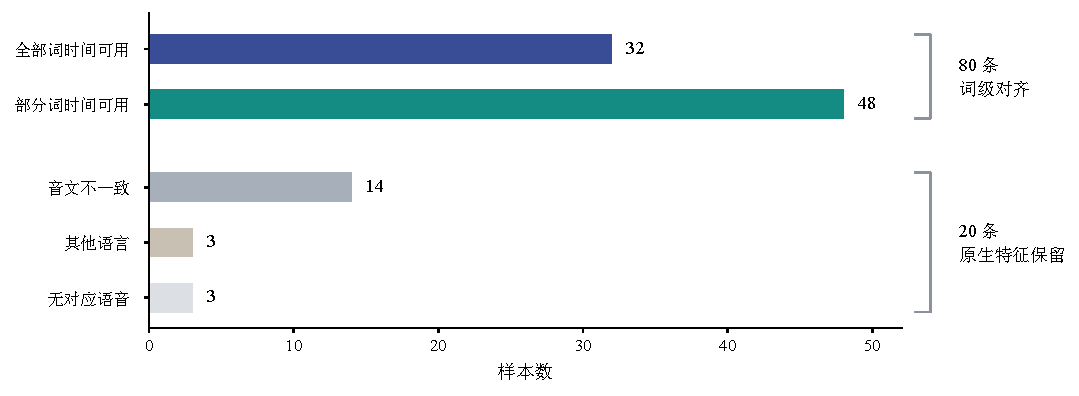
\includegraphics[width=\linewidth]{figures/音文筛查分布.pdf}
 \caption{音文核查与词时间覆盖}
 \label{fig:p1-language-screen}
\end{figure}

\subsubsection{CTC路径与词边界}
使用冻结的wav2vec 2.0英语声学模型\citep{wav2vec2020}，在16 kHz音频上计算字符后验。
官方原文保持不变，对齐用副本统一大小写、标点和数字读法，并保留规范化字符到官方词的映射。
记规范化字符序列为 $c$，第 $t$ 个声学输出位置对字符 $k$ 的后验为 $p_t(k)$，
CTC折叠算子为 $\mathcal B$。依据CTC的路径概率与折叠定义\citep{graves2006ctc}，
本文在给定转写约束下求最大概率路径：
\begin{equation}
 \pi^*=\arg\max_{\pi:\mathcal B(\pi)=c}\sum_t\log p_t(\pi_t).
 \label{eq:p1-ctc-path}
\end{equation}
通过动态规划求解路径。将第 $i$ 个官方词对应字符占用的最早输出帧记为 $l_i$，
最晚输出帧记为 $r_i$，得到
\begin{equation}
 I_i=[a_i,b_i)=[t_0^{(a)}+0.02l_i,\ t_0^{(a)}+0.02(r_i+1)).
 \label{eq:p1-word-interval}
\end{equation}
末端包含最后一个字符占用的全部帧。20 ms为模型输出步长。
对每个字符，先在其占用帧上求后验的几何均值，再对词内字符求算术均值，得到词置信度 $q_i$。

\subsubsection{受转写约束的路径求解}
式~\eqref{eq:p1-ctc-path}中，官方文本限定待寻找的字符顺序，声学后验提供各字符出现位置的证据。
依据CTC的空白符与重复折叠规则\citep{graves2006ctc}，在长度为 $L$ 的目标字符序列两端及相邻字符之间插入空白符，
得到扩展序列 $\boldsymbol c'=(\varnothing,c_1,\varnothing,\ldots,c_L,\varnothing)$。
以下状态下标从0开始，扩展序列长度为 $2L+1$。令 $D_t(j)$ 表示处理至声学帧 $t$、
到达状态 $j$ 的最大对数路径概率；允许的前驱状态集合为
\begin{equation}
 \mathcal P(j)=\{j,j-1\}\cup
 \begin{cases}
 \{j-2\},&j\geq2,\ c'_j\ne\varnothing,\ c'_j\ne c'_{j-2},\\
 \varnothing,&\text{其他情况},
 \end{cases}
 \label{eq:p1-ctc-predecessor}
\end{equation}
其中越界状态从集合中移除。对应递推为
\begin{equation}
 D_t(j)=\log p_t(c'_j)+\max_{k\in\mathcal P(j)}D_{t-1}(k).
 \label{eq:p1-ctc-recursion}
\end{equation}
第一帧仅允许处于起始空白状态或首个字符状态，其余状态设为负无穷。
在最后一帧的末字符状态与末空白状态中选择较优者，沿前驱记录回溯，即可得到最大概率路径。
每个状态最多比较三个前驱，因此时间复杂度为 $O(T_aL)$，其中 $T_a$ 为声学输出帧数；
逐帧评分只需保留相邻两层，回溯记录占 $O(T_aL)$ 空间。

三种转移具有不同含义：停留允许一个字符持续多个输出帧；前进一位允许进入相邻空白或字符；
跨越两位允许相邻不同字符之间省略空白。相邻目标字符相同时，跨越转移被禁止，
否则CTC折叠会把两个相同字符合并为一个。这一约束使路径与给定转写保持一致。
若目标字符数与相邻重复字符所需的最少帧数超过 $T_a$，则该目标在当前音频区间内不可达。

词边界由字符状态的首末占用帧确定，字符之间的空白区间不单独视为一个词。
在短促发音、停顿或重复表达附近，多个可行路径可能具有接近的分数，
最优路径因此仍可能对上下文范围敏感。后续局部复核比较同一词在不同上下文约束下的时间变化，
用于筛除不稳定对应；它与字符后验分别反映边界稳定性和声学支持程度。


\subsubsection{局部复核规则}
本文设置局部复核规则：对每个词选取前后各三个词作为上下文，在初始时间两侧各扩展160 ms重新求解局部路径。
记局部结果为 $(\tilde a_i,\tilde b_i,\tilde q_i)$，候选词须满足
\begin{equation}
 \min(q_i,\tilde q_i)\geq0.50,\qquad
 \max\{|a_i-\tilde a_i|,|b_i-\tilde b_i|\}\leq0.10\ \mathrm{s}.
 \label{eq:p1-word-gate}
\end{equation}
同时检查规范化映射完整、时间在音频覆盖范围内、词序不倒置且已采用的词时间区间不交叠。
完全落入检测静音区间、跨度超过 $\max(1,0.2n_i)$~s或缺少目标字符的词，不采用其候选时间，
其中 $n_i$ 为该词规范化后的字母数。
2条部分内容一致的样本先利用自由识别定位已确认短语，再在短语范围内求解。

通过检查后，以局部复核的起止时间作为最终词区间 $I_i$。
未通过的词保留原位置并单独标记原因，后续词不前移。
局部复核使用同一声学模型，衡量边界对上下文变化的稳定性；
听审未提供独立精确起止标注，因此本文不将上述阈值解释为实际时间误差。

图~\ref{fig:p1-time-selection} 给出词时间筛选的数量与去向。
1932个官方词位置中，20条异常样本包含296个位置，其余80条包含1636个位置。
后者有1533个词时间用于对齐，103个未获得可用时间：82个字符置信度不足，
10个位于听审确认短语之外，6个候选时间完全落入静音区间，4个缺少可供对齐的目标字符，
1个候选时间跨度异常。无目标字符的记录包括独立标点，仍保留其官方位置。

这一筛选将缺乏内容或时间依据的位置排除在词级音视频聚合之外，
同时保留全部原文、原生特征与缺测原因。覆盖统计反映词时间的可用程度，
边界精度仍需独立人工标注评估。
\begin{figure}[!htbp]
\centering
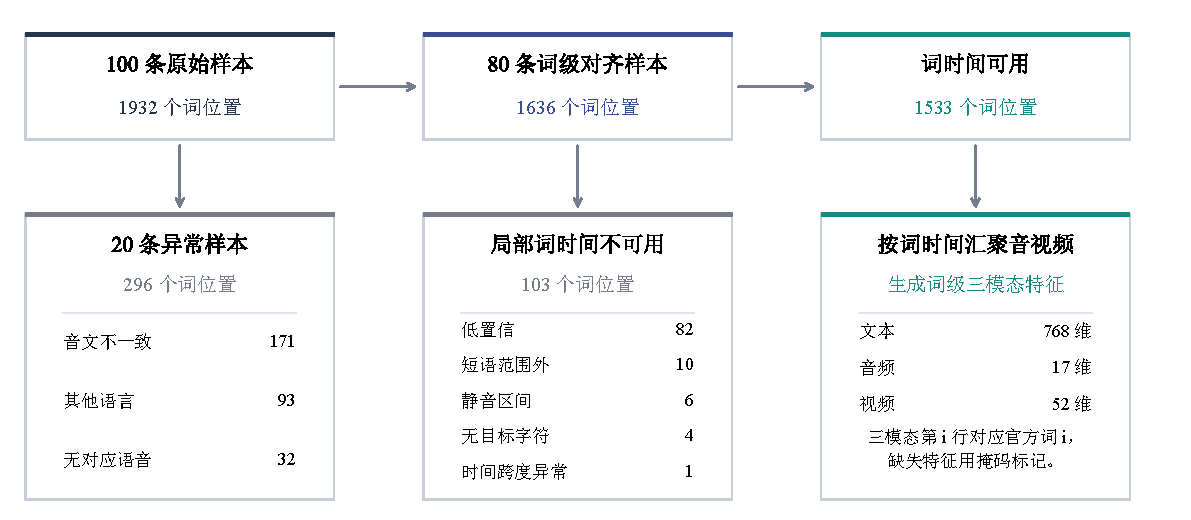
\includegraphics[width=\linewidth]{figures/词时间筛选.pdf}
\caption{词时间筛选与处理去向}
\label{fig:p1-time-selection}
\end{figure}

\subsection{区间交叠聚合与掩码}
设第 $i$ 个词的内容子词集合为 $\mathcal T_i$，词文本特征为
\begin{equation}
 \boldsymbol t_i=\frac{1}{|\mathcal T_i|}\sum_{l\in\mathcal T_i}\boldsymbol h_l.
 \label{eq:p1-word-text}
\end{equation}
文本向量的可用性独立于词时间。对音频窗或视频显示区间 $J_r$，定义交叠长度
$\ell_{ir}=\max(0,\min(b_i,e_r)-\max(a_i,s_r))$。
本文以交叠时长定义汇聚权重，并将逐维可用性纳入归一化。
第 $d$ 维原生特征为 $x_{rd}$，其可用掩码为 $m_{rd}$，则
\begin{equation}
 \bar x_{id}=\frac{\sum_r\ell_{ir}m_{rd}x_{rd}}{\sum_r\ell_{ir}m_{rd}},
 \qquad\sum_r\ell_{ir}m_{rd}>0.
 \label{eq:p1-word-pool}
\end{equation}
该表示也可由局部常量拟合得到。令 $w_{ird}=\ell_{ir}m_{rd}$，用一个数 $z$
代表该词区间内第 $d$ 维的有效观测，最小化加权平方误差
\[
 Q_{id}(z)=\sum_r w_{ird}(x_{rd}-z)^2.
\]
当 $\sum_r w_{ird}>0$ 时，令
$Q'_{id}(z)=2\sum_r w_{ird}(z-x_{rd})=0$，即得到式~\eqref{eq:p1-word-pool}；
且 $Q''_{id}(z)=2\sum_r w_{ird}>0$，故该解唯一。
交叠时长权重是本文对来源贡献的建模选择，上述推导说明其对应的汇聚目标。
分母为零或词时间不可用时，数值填零并将相应观测掩码置为假。
语音17维中，基频只在可测短窗上重新归一化；视频52维只使用单脸有效帧。
所有聚合直接从原生特征计算，保存来源索引、交叠长度和归一化权重。
同一来源窗或显示帧可以支持相邻词，每次贡献由其与该词的交叠长度确定。

对于包含 $N_s$ 个官方词的样本，文本、音频和视频特征矩阵均按官方词序保留 $N_s$ 行，
矩阵形状分别为 $N_s\times768$、$N_s\times17$和$N_s\times52$。
三个矩阵的同一行对应同一个官方词；即使该词缺少可用时间或某一模态的特征，也保留这一行，并通过掩码标记不可用状态。
单文件使用实际序列长度，不添加尾部填充；需要批处理时再补齐，并使用独立结构掩码。
对无可用时间的位置，以缺失值与时间掩码共同记录起止时间。
各类有效性标记与观测状态的含义见表~\ref{tab:p1-npz-fields}。

\begin{table}[htbp]
\centering
\caption{词级序列的有效性与观测状态}
\label{tab:p1-npz-fields}
\begin{tabularx}{\linewidth}{@{}cY@{}}
\toprule
记录 & 含义\\\midrule
词位置有效 & 该位置属于官方词序列，区别于批处理填充\\
词时间可用 & 该词通过时间筛查，可建立音视频对应\\
音频来源与基频可测 & 存在交叠声学窗；基频另行记录可测状态\\
视频来源 & 存在与词区间交叠的真实显示帧\\
面部特征可用 & 至少有单脸有效帧参与该词汇聚\\
内容听审与边界标注 & 分别记录内容核查和独立精确时间标注状态\\
\bottomrule
\end{tabularx}
\end{table}

\subsection{对齐结果与典型样本分析}
\subsubsection{覆盖结果}
完成100条样本的特征提取，共1932个官方词位置、77510个语音短窗和23241个视频显示帧。
100条样本中，80条建立了词级时间对应，共覆盖1533个词，占全部词的79.35\%。
其中32条全部词时间可用，48条部分词时间可用；其余20条按异常类型保留原生特征。
表~\ref{tab:p1-word-coverage} 汇总1533个已对齐词位置的特征可用情况。
采用词时间的所有位置均有音频窗和视频显示帧来源，其中89.63\%取得面部特征。
表中比例以1533个已对齐词位置为分母；159个位置有真实音视频来源，但未取得可用的面部特征。



图~\ref{fig:p1-observation} 展示两种词级覆盖率的经验累积分布。横轴为覆盖率，
纵轴为覆盖率不超过该值的样本比例，两种覆盖率均以每条样本的官方词数为分母。
面部特征曲线位于词时间曲线上方，说明部分已获得词时间的样本仍受到人脸检测缺失或多人帧排除的影响。
浅色区域表示两条累积分布的差距。

\begin{figure}[!htbp]
\centering
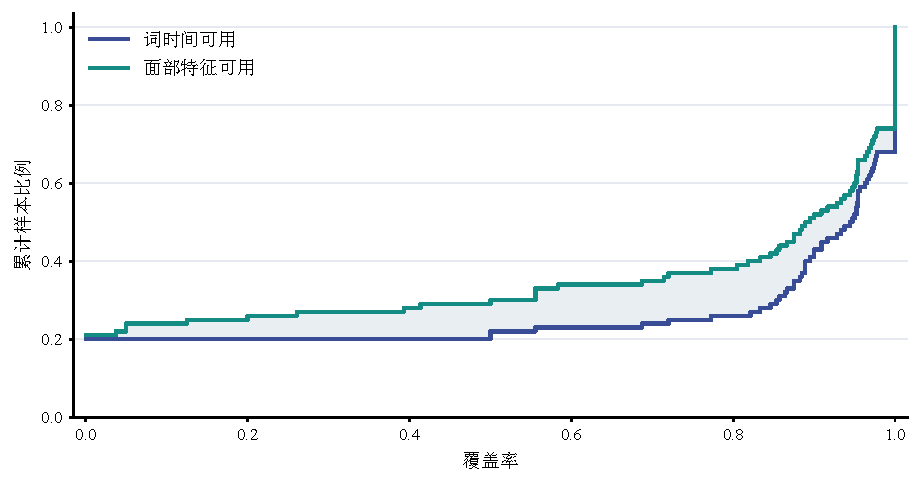
\includegraphics[width=0.98\linewidth]{figures/模态来源概览.pdf}
\caption{词级覆盖率的累积分布}
\label{fig:p1-observation}
\end{figure}

\begin{table}[htbp]
\centering
\caption{已对齐词的三模态特征覆盖}
\label{tab:p1-word-coverage}
\begin{tabularx}{\linewidth}{@{}C{76mm}YY@{}}
\toprule
词级状态 & 词数 & 占比/\% \\
\midrule
三模态特征可用 & 1374 & 89.63 \\
音视频来源可用、面部特征不可用 & 159 & 10.37 \\
\midrule
合计 & 1533 & 100.0 \\
\bottomrule
\end{tabularx}
\end{table}

\subsubsection{典型样本对应关系}
选取样本片段\texttt{-egA8-b7-3M\_9}，官方文本为
“Secondly, another goal of exhibiting is building your company image.”。
该片段包含10个官方词、14个BERT词元、492个语音窗和150个显示帧，10个词均取得三模态特征。
图~\ref{fig:p1-alignment} 在同一媒体时轴上显示词区间、语音能量与面部变化，
上方给出对应视频帧；下方列出每个词所关联的原生观测数量。
原生轨迹在词间停顿处继续保留，词级表示仅汇聚各词实际区间。
\begin{figure}[htbp]
\centering
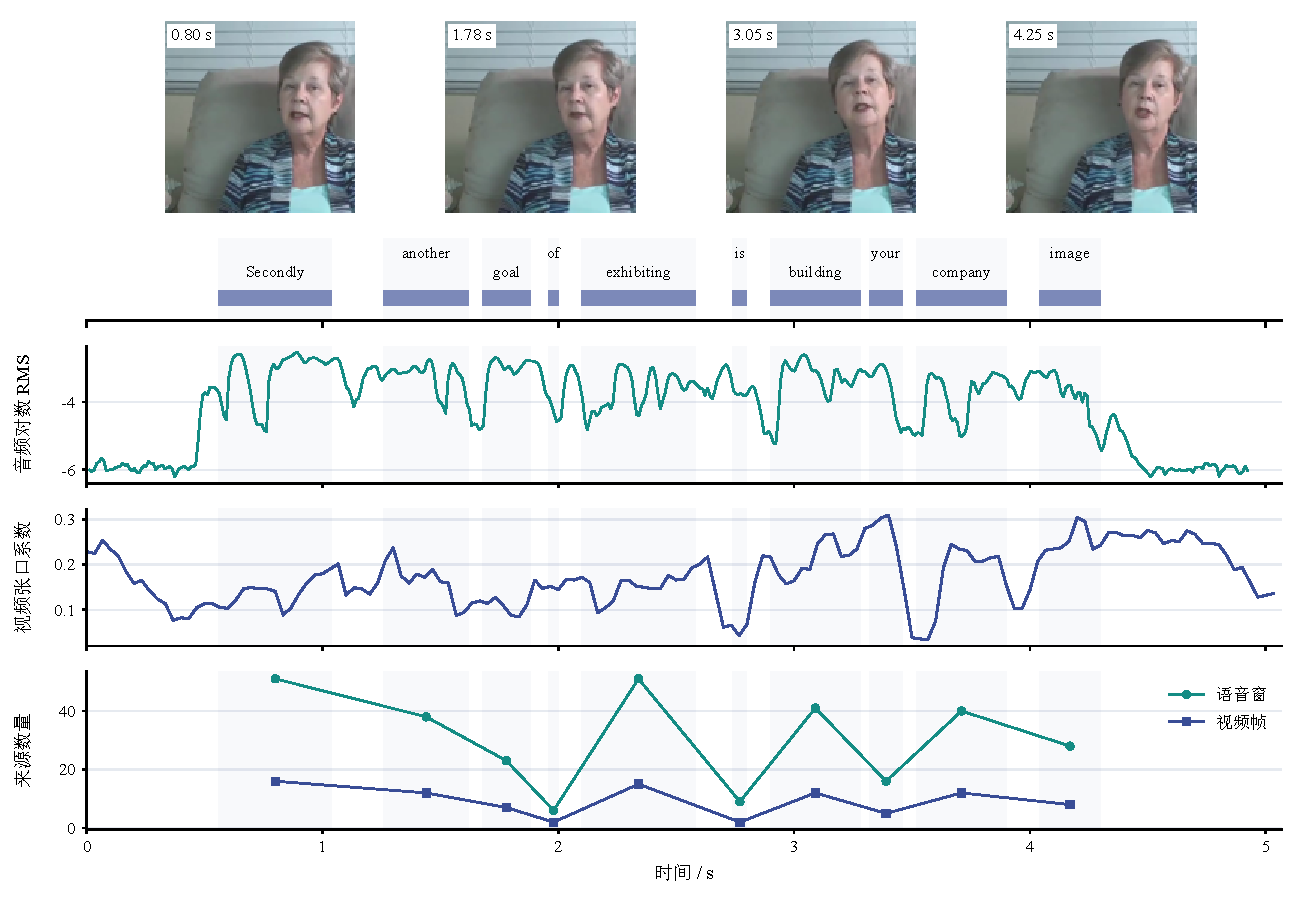
\includegraphics[width=0.98\linewidth]{figures/典型样本对齐.pdf}
\caption{典型样本的词级三模态对应}
\label{fig:p1-alignment}
\end{figure}
该样本10个词的内容与大致位置经试听核对，自动估计的词时间及来源数量见附录表~\ref{tab:appendix-word-times}。

\subsubsection{全部样本的对齐结果}
表~\ref{tab:p1-all-samples} 列出100条样本的三模态共用的词序列长度与实际对齐覆盖。
$T_a$与$T_v$分别为音频和视频的解码覆盖时长，按末帧覆盖终点减去首帧起点计算；
本批样本的两类首帧时间均为0 s，因此覆盖时长与覆盖终点数值相同。
该时长保留静音和未检出人脸的部分。三个矩阵的行数均为该样本的官方词数 $N_s$，
文本、音频、视频的特征维度固定为768、17、52，三个矩阵的形状分别为
$N_s\times768$、$N_s\times17$和$N_s\times52$。
三模态共用官方词序列：第 $i$ 行对应同一个词，词时间被采用后，其音视频特征均由对应区间
$I_i$ 内的原生观测汇聚得到。

共同序列长度 $N_s$ 是保留的全部官方词位置数；对齐词数 $K_s$ 是其中词时间通过筛查、
且有音频窗与视频显示帧来源的位置数；三模态有效词数 $M_s$ 进一步要求该位置的文本、音频及面部特征均可用。
三者满足 $0\le M_s\le K_s\le N_s$。未取得面部特征时，$M_s$ 可以小于 $K_s$；
三个矩阵仍按全部 $N_s$ 个官方词位置组织。
未采用词时间的位置保留官方词与文本表示，音视频词级特征填零并标记不可用；
原生音视频特征另行完整保存。对齐词数为零的样本保留原生特征与样本归属。
文本无独立物理时长，其片段范围由音视频覆盖给出；对齐粒度为所采用的词时间区间。
随附300行逐模态长表另列原生序列长度、模态、维度、解码覆盖时长与对齐状态。
\begingroup
\normalsize\songti
\setlength{\tabcolsep}{3pt}
\begin{longtable}{@{\extracolsep{\fill}}ccccc@{}}
\caption{附件一共同词序列长度与对齐覆盖}\label{tab:p1-all-samples}\\
\toprule
样本片段编号 & $T_a/T_v$/s & 共同序列长度 $N_s$ & 对齐词数 $K_s$ & 三模态有效词数 $M_s$\\\midrule
\endfirsthead
\multicolumn{5}{c}{表\thetable\ （续）}\\\toprule
样本片段编号 & $T_a/T_v$/s & 共同序列长度 $N_s$ & 对齐词数 $K_s$ & 三模态有效词数 $M_s$\\\midrule
\endhead
\bottomrule\endfoot
\texttt{-3g5yACwYnA\_2} & 9.231/9.367 & 14 & 13 & 13 \\
\texttt{-3g5yACwYnA\_3} & 14.33/14.37 & 29 & 28 & 28 \\
\texttt{-3g5yACwYnA\_9} & 8.696/8.8 & 21 & 20 & 20 \\
\texttt{-3g5yACwYnA\_13} & 5.399/5.5 & 15 & 13 & 13 \\
\texttt{-3nNcZdcdvU\_5} & 7.789/7.867 & 18 & 18 & 18 \\
\texttt{-571d8cVauQ\_0} & 4.992/5.167 & 12 & 10 & 10 \\
\texttt{-571d8cVauQ\_5} & 15.12/15.27 & 43 & 42 & 42 \\
\texttt{-6rXp3zJ3kc\_8} & 12.74/12.8 & 34 & 34 & 34 \\
\texttt{-9y-fZ3swSY\_0} & 6.757/6.9 & 22 & 17 & 17 \\
\texttt{-9y-fZ3swSY\_4} & 2.665/2.8 & 9 & 5 & 5 \\
\texttt{-9y-fZ3swSY\_8} & 4.917/4.967 & 12 & 12 & 7 \\
\texttt{-AUZQgSxyPQ\_2} & 22.4/22.5 & 41 & 35 & 35 \\
\texttt{-HeZS2-Prhc\_2} & 8.151/8.233 & 16 & 14 & 14 \\
\texttt{-HwX2H8Z4hY\_2} & 3.916/3.967 & 8 & 4 & 1 \\
\texttt{-HwX2H8Z4hY\_5} & 5.544/5.633 & 10 & 9 & 2 \\
\texttt{-HwX2H8Z4hY\_6} & 3.256/3.333 & 7 & 7 & 5 \\
\texttt{-HwX2H8Z4hY\_9} & 7.636/7.733 & 22 & 19 & 0 \\
\texttt{-I\_e4mIh0yE\_1} & 7.444/7.6 & 18 & 18 & 18 \\
\texttt{-I\_e4mIh0yE\_3} & 8.994/9.133 & 22 & 21 & 21 \\
\texttt{-MeTTeMJBNc\_0} & 9.218/9.333 & 21 & 20 & 20 \\
\texttt{-MeTTeMJBNc\_7} & 10.41/10.5 & 31 & 30 & 30 \\
\texttt{-MeTTeMJBNc\_13} & 5.256/5.4 & 14 & 14 & 14 \\
\texttt{-NFrJFQijFE\_1} & 5.659/5.72 & 16 & 0 & 0 \\
\texttt{-NFrJFQijFE\_2} & 6.698/6.84 & 18 & 0 & 0 \\
\texttt{-RfYyzHpjk4\_2} & 5.392/5.5 & 25 & 18 & 18 \\
\texttt{-RfYyzHpjk4\_8} & 4.532/4.567 & 17 & 15 & 15 \\
\texttt{-RfYyzHpjk4\_11} & 5.075/5.233 & 17 & 17 & 17 \\
\texttt{-THoVjtIkeU\_2} & 4.231/4.267 & 10 & 10 & 10 \\
\texttt{-THoVjtIkeU\_6} & 7.983/8.067 & 30 & 27 & 27 \\
\texttt{-THoVjtIkeU\_12} & 14.81/14.87 & 39 & 38 & 38 \\
\texttt{-UUCSKoHeMA\_0} & 7.732/7.867 & 18 & 17 & 17 \\
\texttt{-UacrmKiTn4\_4} & 4.682/4.733 & 14 & 14 & 14 \\
\texttt{-UacrmKiTn4\_10} & 7.242/7.333 & 18 & 18 & 18 \\
\texttt{-UuX1xuaiiE\_0} & 3.576/3.7 & 9 & 8 & 5 \\
\texttt{-UuX1xuaiiE\_1} & 10.27/10.33 & 27 & 27 & 1 \\
\texttt{-UuX1xuaiiE\_3} & 4.038/4.1 & 9 & 8 & 8 \\
\texttt{-UuX1xuaiiE\_6} & 7.944/8.1 & 22 & 20 & 20 \\
\texttt{-a55Q6RWvTA\_3} & 22.08/22.13 & 65 & 62 & 62 \\
\texttt{-aNfi7CP8vM\_7} & 8.538/8.667 & 18 & 18 & 18 \\
\texttt{-aqamKhZ1Ec\_0} & 10.89/11 & 14 & 7 & 7 \\
\texttt{-dxfTGcXJoc\_0} & 20.41/20.53 & 41 & 40 & 33 \\
\texttt{-dxfTGcXJoc\_1} & 16.02/16.13 & 36 & 35 & 35 \\
\texttt{-dxfTGcXJoc\_2} & 16.63/16.67 & 34 & 33 & 33 \\
\texttt{-dxfTGcXJoc\_6} & 12.63/12.73 & 27 & 26 & 26 \\
\texttt{-egA8-b7-3M\_1} & 10.16/10.23 & 20 & 20 & 20 \\
\texttt{-egA8-b7-3M\_6} & 6.183/6.233 & 12 & 12 & 12 \\
\texttt{-egA8-b7-3M\_9} & 4.936/5.067 & 10 & 10 & 10 \\
\texttt{-egA8-b7-3M\_13} & 4.024/4.167 & 11 & 11 & 11 \\
\texttt{-egA8-b7-3M\_16} & 5.483/5.533 & 11 & 11 & 11 \\
\texttt{-egA8-b7-3M\_17} & 7.095/7.267 & 16 & 16 & 16 \\
\texttt{-egA8-b7-3M\_18} & 8.266/8.367 & 22 & 22 & 22 \\
\texttt{-egA8-b7-3M\_20} & 6.474/6.633 & 20 & 20 & 20 \\
\texttt{-egA8-b7-3M\_26} & 5.921/6 & 15 & 14 & 14 \\
\texttt{-hnBHBN8p5A\_6} & 6.333/6.381 & 13 & 0 & 0 \\
\texttt{-hnBHBN8p5A\_7} & 7.309/7.341 & 13 & 0 & 0 \\
\texttt{-iRBcNs9oI8\_3} & 5.538/5.606 & 8 & 0 & 0 \\
\texttt{-iRBcNs9oI8\_6} & 2.82/2.87 & 5 & 0 & 0 \\
\texttt{-iRBcNs9oI8\_7} & 4.006/4.071 & 9 & 0 & 0 \\
\texttt{-iRBcNs9oI8\_8} & 8.026/8.075 & 21 & 0 & 0 \\
\texttt{-iRBcNs9oI8\_9} & 3.374/3.403 & 5 & 0 & 0 \\
\texttt{-lzEya4AM\_4\_5} & 7.57/7.667 & 19 & 17 & 17 \\
\texttt{-lzEya4AM\_4\_6} & 14.74/14.77 & 43 & 41 & 41 \\
\texttt{-mJ2ud6oKI8\_1} & 6.055/6.073 & 13 & 0 & 0 \\
\texttt{-mJ2ud6oKI8\_2} & 5.702/5.706 & 11 & 0 & 0 \\
\texttt{-mJ2ud6oKI8\_6} & 2.228/2.236 & 5 & 0 & 0 \\
\texttt{-mJ2ud6oKI8\_8} & 4.171/4.171 & 11 & 0 & 0 \\
\texttt{-mJ2ud6oKI8\_9} & 6.909/7.007 & 22 & 0 & 0 \\
\texttt{-mqbVkbCndg\_0} & 6.385/6.5 & 12 & 12 & 12 \\
\texttt{-qDkUB0GgYY\_6} & 4.615/4.667 & 16 & 11 & 11 \\
\texttt{-ri04Z7vwnc\_0} & 2.763/2.794 & 8 & 0 & 0 \\
\texttt{-ri04Z7vwnc\_2} & 5.913/6.006 & 16 & 0 & 0 \\
\texttt{-ri04Z7vwnc\_5} & 3.44/3.503 & 9 & 0 & 0 \\
\texttt{-s9qJ7ATP7w\_0} & 6.711/6.867 & 24 & 21 & 21 \\
\texttt{-s9qJ7ATP7w\_1} & 4.644/4.767 & 11 & 10 & 9 \\
\texttt{-s9qJ7ATP7w\_4} & 4.247/4.4 & 9 & 8 & 5 \\
\texttt{-s9qJ7ATP7w\_5} & 8.398/8.533 & 19 & 18 & 18 \\
\texttt{-s9qJ7ATP7w\_6} & 2.315/2.467 & 5 & 5 & 5 \\
\texttt{-s9qJ7ATP7w\_7} & 6.839/6.933 & 28 & 23 & 11 \\
\texttt{-s9qJ7ATP7w\_8} & 3.184/3.267 & 13 & 11 & 11 \\
\texttt{-t217m2on-s\_2} & 5.63/5.667 & 12 & 11 & 11 \\
\texttt{-t217m2on-s\_7} & 17.03/17.17 & 45 & 44 & 44 \\
\texttt{-tANM6ETl\_M\_3} & 6.604/6.733 & 22 & 21 & 21 \\
\texttt{-tPCytz4rww\_10} & 4.679/4.767 & 12 & 12 & 12 \\
\texttt{-tPCytz4rww\_11} & 5.379/5.467 & 17 & 17 & 17 \\
\texttt{-tPCytz4rww\_12} & 11.74/11.83 & 26 & 23 & 23 \\
\texttt{-tPCytz4rww\_16} & 7.139/7.2 & 16 & 15 & 15 \\
\texttt{-tPCytz4rww\_18} & 6.569/6.633 & 16 & 16 & 16 \\
\texttt{-uywlfIYOS8\_4} & 5.881/6.033 & 18 & 18 & 18 \\
\texttt{-vxjVxOeScU\_4} & 9.037/9.1 & 21 & 18 & 18 \\
\texttt{-wMB\_hJL-3o\_7} & 5.976/6.033 & 22 & 22 & 22 \\
\texttt{-wny0OAz3g8\_0} & 3.274/3.333 & 9 & 9 & 9 \\
\texttt{-wny0OAz3g8\_1} & 6.777/6.833 & 23 & 22 & 6 \\
\texttt{-wny0OAz3g8\_2} & 6.523/6.667 & 23 & 23 & 23 \\
\texttt{-wny0OAz3g8\_3} & 6.1/6.133 & 20 & 20 & 1 \\
\texttt{-wny0OAz3g8\_5} & 6.741/6.9 & 20 & 20 & 1 \\
\texttt{-wny0OAz3g8\_7} & 7.91/8.067 & 29 & 29 & 12 \\
\texttt{-wny0OAz3g8\_9} & 6.043/6.2 & 20 & 19 & 19 \\
\texttt{-yRb-Jum7EQ\_1} & 29.11/29.27 & 49 & 0 & 0 \\
\texttt{-yRb-Jum7EQ\_5} & 13.04/13.17 & 25 & 0 & 0 \\
\texttt{-yRb-Jum7EQ\_6} & 11.24/11.2 & 19 & 0 & 0 \\
\end{longtable}
\endgroup

\subsection{特征一致性与聚合性质}
每条样本的原生序列、词级特征、时间及观测掩码均与样本片段编号关联。
100条样本的官方词位置全部保留，时间范围、先后顺序及观测掩码均满足前述定义。
特征以每样本一个压缩NPZ文件组织，按样本片段编号读取原生序列、三个词级矩阵及其掩码；实际长度与来源映射随特征保存，批处理时依据结构掩码区分填充位置。
依据来源索引和聚合权重重新计算1533个对齐词的特征，所得结果与存储值在浮点精度容限内一致；
23241个视频显示帧的来源位置也与解码记录一致。这些检查验证了特征表示与计算规则的一致性。

特征提取模型采用推理模式，参数保持冻结。工具版本、核心参数和使用场景见附录表~\ref{tab:appendix-tools}，
特征文件组织及复现材料见附录~\ref{sec:appendix-runtime}。

对任一有效特征维 $d$，记归一化权重为
$\omega_{ird}=w_{ird}/\sum_r w_{ird}$，则 $\omega_{ird}\geq0$ 且 $\sum_r\omega_{ird}=1$。
因此 $\bar x_{id}$ 是有效来源值的凸组合，位于这些来源值的最小值与最大值之间。
在词边界、来源集合、掩码及权重固定时，由三角不等式有
\[
 |\delta\bar x_{id}|=
 \left|\sum_r\omega_{ird}\delta x_{rd}\right|
 \leq\sum_r\omega_{ird}|\delta x_{rd}|
 \leq\max_{r,d'}|\delta x_{rd'}|.
\]
再对有效维度取最大值，得到
$\|\delta\bar{\boldsymbol x}_i\|_\infty\leq\max_r\|\delta\boldsymbol x_r\|_\infty$。
该结论约束固定映射下的特征数值扰动；词边界或有效来源改变时需重新分析。

\subsubsection*{（1）词边界变化对汇聚结果的影响}
对同一词和特征维，设两种边界对应的归一化权重为 $\omega_r$ 与 $\omega'_r$，
在两组来源的并集上补零，使两者均满足权重和为1。若并集中的原生特征值满足
$x_{\min}\leq x_r\leq x_{\max}$，则两种汇聚结果之差可写为
\begin{equation}
 \left|\bar x'-\bar x\right|
 =\left|\sum_r(\omega'_r-\omega_r)(x_r-c)\right|
 \leq\frac{x_{\max}-x_{\min}}{2}\sum_r|\omega'_r-\omega_r|,
 \quad c=\frac{x_{\max}+x_{\min}}{2}.
 \label{eq:p1-weight-stability}
\end{equation}
等式利用 $\sum_r(\omega'_r-\omega_r)=0$，不等式由三角不等式及
$|x_r-c|\leq(x_{\max}-x_{\min})/2$ 得到。该推导以原生特征和其有效性不变、
两组权重的分母均为正为前提，说明边界变化的影响同时取决于权重分布变化和来源特征的变化幅度。
若边界只在相近特征值之间移动，汇聚结果可能变化较小；若跨过明显的声学或面部变化，
即使时间移动不大，结果也可能受到较强影响。因此，时间误差与表示误差需要分别评价。

\subsubsection*{（2）观测密度与对齐粒度}
音频采用25 ms分析窗和10 ms步长，相邻窗口存在交叠；视频显示区间则按实际帧时间组织。
词区间内的音频窗数通常大于视频帧数，这由特征采样方式决定。
两种模态只需对应同一词区间，并不要求具有相同的原生观测数量。
对于短于一帧显示时长的词，显示起点位于词前方的画面仍可能覆盖该词；
以区间交叠确定来源，可保留这部分真实显示信息。
相邻词复用同一音频窗或视频帧时，其表示可能相关，因此来源数量不能直接解释为独立观测数。

均值汇聚会压缩词内的变化顺序，因此同时保存原生序列。
当前质量限制主要来自音文不一致、词边界不确定以及面部检测失效；
词时间误差还需要独立边界标注评估，25 ms短窗也限制低基频的测量稳定性。

% ==================== problem2
\section{问题二：局部模态缺失下的鲁棒情感预测}
\label{sec:problem2}

\subsection{问题分析与建模目标}

问题二要求同时给出离散情感极性和连续情感强度，并重点考察复杂场景下局部模态
不可用时的预测能力。与完整三模态分类相比，本问有三项额外困难。其一，三种模态
在同一位置的数值为零可能分别代表填充、自然未观测或人为遮挡，若不保留掩码，
模型无法区分这些状态。其二，文本、语音和视频的信息量不均衡；若直接拼接，模型
容易依赖文本，在文本缺失时发生明显退化。其三，三分类标签和连续强度来源于同一
情感标注，二者的符号应当一致，但普通双头网络可能输出“正向类别、负强度”等矛盾结果。

据此，将问题形式化为带观测掩码的多任务学习。对于样本 $s$，输入为
\begin{equation}
 \mathcal X_s=\{X_s,A_s,V_s,M_s^x,M_s^a,M_s^v,M_s^{\rm str}\},
 \label{eq:p2-input}
\end{equation}
其中 $X_s\in\mathbb R^{50\times768}$、$A_s\in\mathbb R^{50\times74}$、
$V_s\in\mathbb R^{50\times35}$ 分别为文本、语音和视频序列，$M_s^{\rm str}$
为结构有效掩码，$M_s^q$ 为模态 $q$ 的观测掩码。文本序列由附件中的BERT词元输入经冻结编码器得到，
发生文本遮挡时重新编码。输出为三分类概率
$\hat{\boldsymbol p}_s\in[0,1]^3$ 和强度 $\hat y_s\in[-3,3]$。
类别编码为 $0,1,2$，依次表示负向、中性和正向，真实强度 $y_s$ 与类别满足
\begin{equation}
 c_s=\begin{cases}0,&y_s<0,\\1,&y_s=0,\\2,&y_s>0.\end{cases}
 \label{eq:p2-label-relation}
\end{equation}

本文的总体思路为：先严格分离结构掩码与观测掩码；再在训练集结构有效区间内
模拟不同位置、长度和模态组合的连续缺失；分别建立文本专家和音视频专家；最后依据
当前观测比例和语义表示学习样本级门控，并联合优化分类、回归、分支监督和跨模态
辅助重构。模型固定后，以完整输入和统一的缺失压力测试共同评价，再对附件三推理。

\subsection{数据版本、划分与掩码}

\subsubsection{数据版本选择}

附件二同时给出对齐版和未对齐版。对齐版的三种模态均为最多 $50$ 个位置，且附件三
对齐版提供相同形式的词元输入、$74$ 维语音和 $35$ 维视频；未对齐版的音视频为
$500$ 个位置，附件三未对齐版又缺少与训练集相同的词元字段和可靠长度字段。
本文因此采用对齐版特征，使模型训练和附件三预测使用相同的序列组织方式。

附件二训练、验证和测试分别含 $3395$、$728$ 和 $727$ 条样本。本文只用训练集
拟合网络参数、音视频标准化统计量和类别权重，只用验证集选择结构、轮次和方法；
测试集及附件三、四的无标签样本均不参与模型选择。

\begin{table}[htbp]
 \centering
 \caption{对齐版三模态输入与掩码定义}
 \label{tab:p2-data-interface}
 \begin{tabular*}{\linewidth}{@{\extracolsep{\fill}}cccc@{}}
 \toprule
 模态 & 单样本形状 & 结构长度依据 & 观测状态依据 \\
 \midrule
 文本 & $50\times768$ & BERT注意力掩码 & 内容词元掩码 \\
 语音 & $50\times74$ & 文本对齐有效区间 & 结构区间内非零行 \\
 视频 & $50\times35$ & 文本对齐有效区间 & 结构区间内非零行 \\
 \bottomrule
 \end{tabular*}
\end{table}

\subsubsection{结构有效、自然未观测与人工缺失}

对文本，BERT注意力掩码给出结构有效前缀；首尾特殊词元
\texttt{[CLS]}、\texttt{[SEP]} 仍属于结构序列，但不计为可遮挡的内容词元。
附件中的文本向量在填充位置可能非零，因此不能用零向量推断文本长度。
对音频和视频，结构区间内全零行记为未观测，但不推断其物理原因；结构区间之外统一
视为尾部填充。记 $\mathcal O_s^q$ 为样本 $s$ 中满足模态 $q$ 观测判据的位置集合：
文本取内容词元位置，音视频取标准化前原始特征的非零行位置。
以 $\mathbf 1\{\cdot\}$ 表示条件成立时取1、否则取0的指示函数，则
\begin{equation}
 M^q_{s,t}=M^{\rm str}_{s,t}\mathbf 1\{t\in\mathcal O_s^q\},
 \qquad M^q_{s,t}\le M^{\rm str}_{s,t}.
 \label{eq:p2-mask-contract}
\end{equation}
人工缺失再由增强掩码 $D^q_{s,t}\in\{0,1\}$ 表示，模型实际接收的掩码为
\begin{equation}
 \widetilde M^q_{s,t}=M^q_{s,t}(1-D^q_{s,t}).
 \label{eq:p2-effective-mask}
\end{equation}
这样，尾部填充不被计作一次缺失，自然全零位置也不会在增强时重复计数。

\subsubsection{训练集统计量与标准化}

采用按特征维标准化的常规预处理\citep{goodfellow2016deep}，
仅在训练集观测位置估计音视频每维均值 $\mu_{q,j}$ 与标准差 $\sigma_{q,j}$：
\begin{equation}
 \mu_{q,j}=\frac{\sum_{s,t}M^q_{s,t}Z^q_{s,t,j}}{\sum_{s,t}M^q_{s,t}},\qquad
 \sigma_{q,j}^2=\frac{\sum_{s,t}M^q_{s,t}(Z^q_{s,t,j}-\mu_{q,j})^2}
 {\sum_{s,t}M^q_{s,t}},
 \label{eq:p2-standardization}
\end{equation}
标准差下限取 $\bar\sigma_{q,j}=\max(\sigma_{q,j},10^{-4})$，并令
\[
 \widetilde Z^q_{s,t,j}=\operatorname{clip}_{[-10,10]}
 \left(\frac{Z^q_{s,t,j}-\mu_{q,j}}{\bar\sigma_{q,j}}\right).
\]
未观测位置在标准化后保持为零，并始终由掩码排除。验证集和附件三、四固定使用训练集
统计量，不重新估计。

三分类存在不均衡。为降低多数类对交叉熵的影响，本文根据训练集类别频数 $n_c$ 设置权重：
\begin{equation}
 w_c=\frac{n_c^{-1/2}}{\frac13\sum_{j=0}^{2}n_j^{-1/2}}.
 \label{eq:p2-class-weight}
\end{equation}
该归一化使三类权重的算术均值为1。平方根倒数提高少数类的相对权重，
相较完全倒数又缩小了类别之间的权重差距；本文将其作为类别平衡的设置。

\subsection{连续局部缺失的数学构造}

\subsubsection{缺失片段生成}

随机缺失增强已用于不完整多模态情感学习\citep{wang2025distill}。本文将缺失单元设为连续片段，
训练时以概率 $0.7$ 对样本执行缺失增强。设模态 $q$ 的可观测位置按时间排序为
$\mathcal I_s^q=(i_1,\ldots,i_{L_q})$，从 $[0.15,0.40]$ 均匀采样缺失比例
$\rho$，长度为
\begin{equation}
 \ell_q=\max\{1,\min(L_q,\operatorname{round}_{\rm even}(\rho L_q))\}.
 \label{eq:p2-drop-length}
\end{equation}
$\operatorname{round}_{\rm even}$ 表示取最近整数，恰为半整数时取相邻偶数；空观测模态不执行遮挡。再均匀采样起点 $b_q\in\{0,\ldots,L_q-\ell_q\}$，令
$D^q_{s,i_r}=1$，其中 $b_q<r\le b_q+\ell_q$。约 $20\%$ 的增强样本同时
遮挡两个模态，其余遮挡一个模态；另有约 $10\%$ 的批内样本遮挡全部文本，
迫使音视频专家获得独立监督。连续遮挡比独立随机置零更接近转写中断、麦克风失效、
人脸暂时离开画面等实际缺失。

预计算文本向量包含双向上下文，未遮位置可能已经编码被遮词信息。为消除该信息泄漏，
先把对应词元替换为 \texttt{[MASK]}，
再送入冻结 BERT 重新编码。音频和视频则同步将缺失区间数值置零并更新观测掩码。

\subsubsection{验证压力场景}

为使不同模型在完全相同的条件下比较，验证时不用随机缺失，而固定设计
$3\times2\times3=18$ 个单模态局部缺失场景：模态为文本、语音、视频；长度为
$20\%$、$40\%$；位置为首部、中部、尾部。令 $L$ 为当前模态的已观测位置数，起点是这些位置按时间排序后的序号，三种起点分别取
\begin{equation}
 b_{\rm start}=0,\qquad b_{\rm middle}=\left\lfloor\frac{L-\ell}{2}\right\rfloor,
 \qquad b_{\rm end}=L-\ell.
 \label{eq:p2-fixed-position}
\end{equation}
另设置三个整模态剔除场景，检验模型在极端情况下的退化。所有场景都在同一批
$728$ 条验证样本上重新推理，因而场景差异不来自样本构成变化。

\subsection{文本—音视频混合专家模型}

本文借鉴MoE的专家分工与门控组合结构\citep{jacobs1991moe}，
设置文本专家和音视频专家，分别输出三分类logits与连续情感强度。
采用样本级稠密门控：每次前向计算两个专家的输出，再以非负权重 $g_s$ 和 $1-g_s$ 加权。
门控在每个样本上产生一个标量，作用于整组分类logits和回归输出。
下文将该结构称为文本—音视频混合专家模型；加入文本表示辅助重构后的版本称为文本表征引导MoE。

图~\ref{fig:p2-architecture} 给出最终模型的网络结构。文本专家使用冻结 BERT，结构掩码控制其注意力范围，
观测掩码限定参与词元均值的内容位置。音频与视频分别通过64维残差一维卷积、掩码均值与注意力池化，
再拼接观测比例并组成音视频专家；两个专家各自具有分类头
和回归头。门控网络读取专家隐表示与三模态观测比例，对两组预测输出加权。
图中 $z^x$ 和 $r^{av}$ 分别对应文本与音视频专家隐表示，门控输入处沿用同名表示；
标注“仅训练”的虚线将音视频专家连接到下方文本表征引导分支，重构输出与停止梯度的文本目标共同
计算 MSE，该辅助损失仅在文本未遮挡的样本上计算。主任务与两专家分支另按联合损失接受监督。
单个MoE中的两个专家共同训练，融合权重由门控网络逐样本计算；
最终集成包含三个独立随机种子训练的MoE，分别平均它们的分类logits与原始强度，再执行符号一致性投影。
\begin{figure}[htbp]
 \centering
 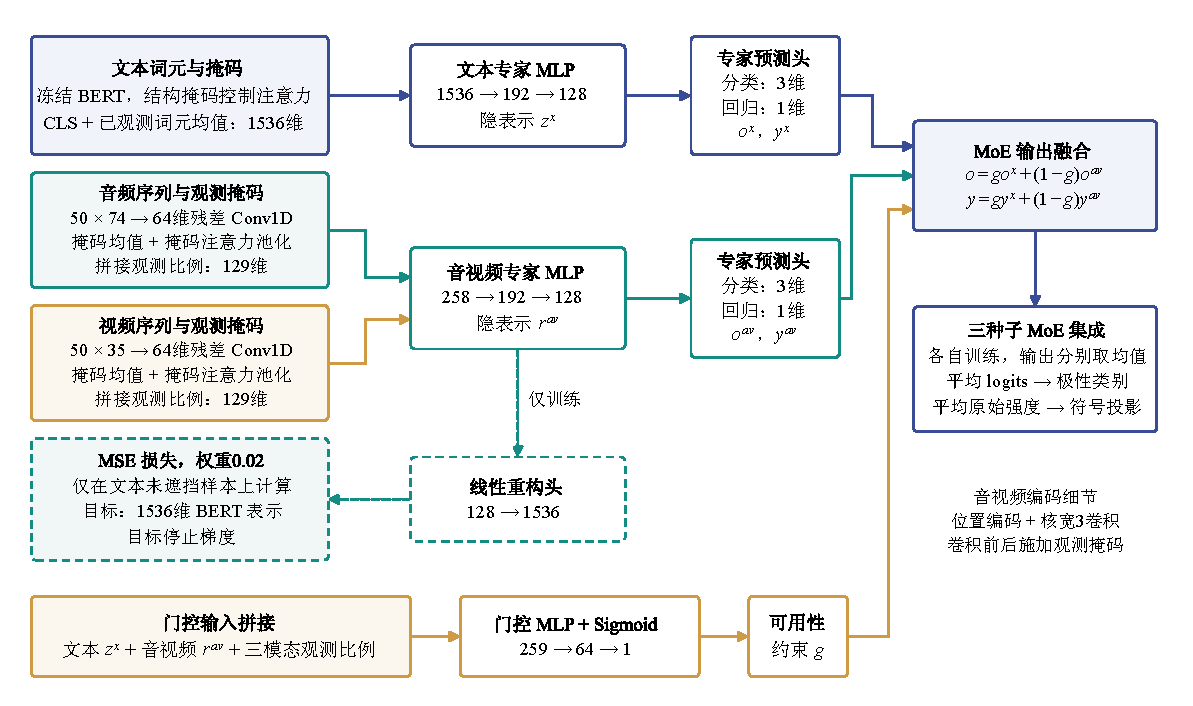
\includegraphics[width=0.98\linewidth]{figures/混合专家模型框架.pdf}
 \caption{文本表征引导的混合专家网络}
 \label{fig:p2-architecture}
\end{figure}

\subsubsection{文本语义专家}

文本分支采用冻结的 \texttt{bert-base-uncased}\citep{bert_acl_online}。

设遮挡后最后层输出为 $H_s^x=(\boldsymbol h_{s,1},\ldots,\boldsymbol h_{s,50})$，
本文将首位 \texttt{[CLS]} 向量和已观测内容词元均值拼接：
\begin{equation}
 \boldsymbol r_s^x=\left[\boldsymbol h_{s,\rm CLS};
 \frac{\sum_t\widetilde M^x_{s,t}\boldsymbol h_{s,t}}
 {\max(1,\sum_t\widetilde M^x_{s,t})}\right]\in\mathbb R^{1536}.
 \label{eq:p2-text-repr}
\end{equation}
冻结BERT可减少可训练参数，并降低小样本条件下微调的不稳定性。
文本多层感知机依次为 $1536\to192$ 线性层、LayerNorm\citep{ba2016layernorm}、
GELU\citep{hendrycks2016gelu}、
丢弃率0.25的Dropout\citep{goodfellow2016deep}、$192\to128$线性层及GELU，得到隐表示 $\boldsymbol z_s^x$；
两个线性输出头分别输出
分类对数值 $\boldsymbol o_s^x$ 与强度 $\hat y_s^x$。

\subsubsection{音视频时序专家}

对语音和视频分别进行64维线性投影、层归一化和GELU激活，加入可训练位置编码后
乘观测掩码，再通过核宽为3的单层残差一维卷积与GELU激活。残差相加借鉴残差学习结构\citep{he2016residual}。卷积输出再次乘掩码，
以保留缺失位置的零状态。注意力汇聚采用可学习打分、softmax归一化与加权求和的思路\citep{yang2016attention}；
本文使用线性打分并加入观测掩码。对模态 $q\in\{a,v\}$，同时计算掩码均值与注意力池化：
\begin{equation}
 \begin{aligned}
 \boldsymbol u_s^q&=\frac{\sum_t\widetilde M^q_{s,t}\boldsymbol e^q_{s,t}}
 {\max(1,\sum_t\widetilde M^q_{s,t})},\qquad
 \boldsymbol h_s^q=\sum_t\alpha^q_{s,t}\boldsymbol e^q_{s,t},\\
 \alpha^q_{s,t}&=\frac{\widetilde M^q_{s,t}\exp(\boldsymbol w_q^\top\boldsymbol e^q_{s,t})}
 {\sum_j\widetilde M^q_{s,j}\exp(\boldsymbol w_q^\top\boldsymbol e^q_{s,j})}.
 \end{aligned}
 \label{eq:p2-av-pool}
\end{equation}
若整个模态不可用，两种池化向量均置零。每种模态的两组64维池化向量与一个观测比例
拼接为129维表示；语音与视频合并为258维，再经 $258\to192\to128$ 的多层感知机
得到音视频专家表示 $\boldsymbol r_s^{av}$，产生分类对数值 $\boldsymbol o_s^{av}$
与强度 $\hat y_s^{av}$。该分支独立接受分类和回归监督。

\subsubsection{观测掩码驱动的动态门控}

模态门控与动态融合的研究\citep{miao2023gating,wei2024nontext,chen2026experts}为自适应加权提供依据。
本文将预测分为文本和音视频两个专家，门控同时读取专家表示与观测比例，并明确全缺失时的分支规则。
按固定50个输入位置计算三种模态观测比例
\begin{equation}
 \rho_s^q=\frac{1}{50}\sum_{t=1}^{50}\widetilde M^q_{s,t},
 \qquad q\in\{x,a,v\}.
 \label{eq:p2-observed-ratio}
\end{equation}
门控网络 $f_g$ 为 $259\to64\to1$ 的两层感知机，中间采用GELU，
读取两个专家表示与 $\boldsymbol\rho_s=(\rho_s^x,\rho_s^a,\rho_s^v)$：
\begin{equation}
 g_s^{(0)}=\sigma\!\left(f_g([\boldsymbol z_s^x;\boldsymbol r_s^{av};\boldsymbol\rho_s])\right),
 \label{eq:p2-gate-value}
\end{equation}
令 $A_s^{av}=\mathbf1\{\rho_s^a+\rho_s^v>0\}$，
$A_s^x=\mathbf1\{\rho_s^x>0\}$。最终门控按互斥分支定义为
\[
 g_s=\begin{cases}
 1,& A_s^{av}=0,\\
 0,& A_s^{av}=1,\ A_s^x=0,\\
 g_s^{(0)},& A_s^{av}=A_s^x=1.
 \end{cases}
\]
再融合两个专家输出：
\begin{equation}
 \boldsymbol o_s=g_s\boldsymbol o_s^x+(1-g_s)\boldsymbol o_s^{av},\qquad
 \hat y_s=g_s\hat y_s^x+(1-g_s)\hat y_s^{av}.
 \label{eq:p2-gate}
\end{equation}
文本不可用而音视频仍可用时取 $g_s=0$；音视频均不可用时取 $g_s=1$，包括三模态均不可用的空输入。空输入时文本内容全部被遮挡，仍由该固定分支产生基线输出。
这些边界条件使模型在整模态缺失时仍有确定行为。其余情况下，$g_s$ 由数据学习，
故相同缺失比例的不同样本可以获得不同融合权重。

\subsubsection{融合输出的概率含义}
本文在分类logits上进行加权，随后通过softmax得到类别概率。由softmax定义\citep{goodfellow2016deep}，
令 $p_{s,c}^x$ 和 $p_{s,c}^{av}$ 分别为两个专家对类别 $c$ 的预测概率，则
\begin{equation}
 p_{s,c}=\frac{(p_{s,c}^x)^{g_s}(p_{s,c}^{av})^{1-g_s}}
 {\sum_j(p_{s,j}^x)^{g_s}(p_{s,j}^{av})^{1-g_s}}.
 \label{eq:p2-geometric-pooling}
\end{equation}
具体地，将 $o_{s,c}^q=\log p_{s,c}^q+\log Z_s^q$ 代入式~\eqref{eq:p2-gate}，
其中 $Z_s^q=\sum_j\exp(o_{s,j}^q)$，归一化时与类别无关的项相消，即得上式。
因此分类输出是两个专家概率的归一化加权几何平均；原始强度仍按式~\eqref{eq:p2-gate}进行算术加权。
两种输出对应不同的融合运算，门控值直接控制的是分类logits和回归输出的权重。

三个完整MoE的logits再次取算术平均时，同理可得最终类别概率
正比于三个单模型概率乘积的三次方根。各模型预测同一类别时，该类别得到共同支持；
模型之间存在分歧时，最终排序取决于三组概率的共同作用。
这也解释了为何先平均logits再评价，与先评价各模型再平均指标不能互换。

\subsubsection{跨模态辅助重构}

特征重构可作为缺失模态学习的辅助约束\citep{mcthfr2024}。本文将目标设为冻结BERT的片段表示，
增加从 $\boldsymbol r_s^{av}$ 到完整
文本表示的辅助重构头 $R(\cdot)$。目标向量只由训练集未遮挡文本计算，并停止梯度：
\begin{equation}
 \mathcal L_{\rm rec}=\frac{1}{1536|\mathcal C|}\sum_{s\in\mathcal C}
 \left\|R(\boldsymbol r_s^{av})-\operatorname{sg}(\boldsymbol r_{s,\rm full}^x)\right\|_2^2.
 \label{eq:p2-reconstruction}
\end{equation}
其中 $\mathcal C$ 为当前训练批次内文本未被遮挡的样本集合；集合为空时该项为零。
该损失按样本和1536个表示维度共同取均值。
该辅助任务仅在表示空间施加训练约束，鼓励音视频专家学习与文本语义相关的方向；
推理时直接使用音视频专家的表示与预测输出。

\subsection{联合损失与训练算法}

\subsubsection{分类、回归及分支监督}

主分类损失采用softmax交叉熵\citep{goodfellow2016deep}，并加入本文设定的类别权重：
\begin{equation}
 \mathcal L_{\rm cls}=-\frac{1}{\sum_s w_{c_s}}\sum_s w_{c_s}
 \log\frac{\exp(o_{s,c_s})}{\sum_{j=0}^{2}\exp(o_{s,j})}.
 \label{eq:p2-cls-loss}
\end{equation}
强度回归采用 SmoothL1\citep{girshick2015fast}。令误差 $e_s=\hat y_s-y_s$，则
\begin{equation}
 \mathcal L_{\rm reg}=\frac1N\sum_s
 \begin{cases}\frac12e_s^2,&|e_s|<1,\\|e_s|-\frac12,&|e_s|\ge1.
 \end{cases}
 \label{eq:p2-reg-loss}
\end{equation}
相比平方误差，它降低少数强度离群点对梯度的支配。文本和音视频专家各计算同形式的
辅助分类与回归损失。音视频分支取
$\mathcal L_{av}=\mathcal L_{{\rm cls},av}+0.2\mathcal L_{{\rm reg},av}$，
文本分支仅在 $\mathcal A_x=\{s:A_s^x=1\}$ 上取
$\mathcal L_x=\mathcal L_{{\rm cls},x}+0.2\mathcal L_{{\rm reg},x}$。
各分支的分类项按各自样本集合的标签权重和归一化，回归项按该集合样本数取均值；
$\mathcal A_x$ 为空时 $\mathcal L_x=0$。本文将上述任务组合为联合目标，各项系数按验证集选模方案固定：
\begin{equation}
 \mathcal L=\mathcal L_{\rm cls}+0.2\mathcal L_{\rm reg}
 +0.2\mathcal L_x+0.3\mathcal L_{av}+0.02\mathcal L_{\rm rec}.
 \label{eq:p2-total-loss}
\end{equation}
优化器为 AdamW\citep{loshchilov2019adamw}，学习率 $3\times10^{-4}$，批量大小为 $64$，随机种子为
$2026,2027,2028$。

\subsubsection{模型选择与集成}

只按完整输入 Macro-F1 选择模型，可能牺牲缺失鲁棒性和回归效果；只按缺失场景选择，
又可能降低正常输入性能。因此本文以完整输入Macro-F1为主项，
加入文本中部缺失表现及回归指标作为折中项，预先定义综合选模分数
\begin{equation}
 S=\text{Macro-F1}^{\mathrm{full}}
 +0.25\text{Macro-F1}^{\mathrm{text\ mid40}}
 +0.1r^{\mathrm{full}}-0.1\operatorname{MAE}^{\mathrm{full}}.
 \label{eq:p2-selection}
\end{equation}
每个随机种子独立选取 $S$ 最大的训练轮次，再将三个模型的分类对数值和原始强度分别
作算术平均，采用多模型平均的集成思路\citep{goodfellow2016deep}。式~\eqref{eq:p2-selection} 中的Pearson与MAE均为符号投影前的回归指标。
集成预测过程为
\[
 \bar{\boldsymbol o}_s=\frac13\sum_{k=1}^3\boldsymbol o_s^{(k)},\quad
 \hat{\boldsymbol p}_s=\operatorname{softmax}(\bar{\boldsymbol o}_s),\quad
 \hat c_s=\arg\max_j\hat p_{s,j},\quad
 \hat y_s^{\rm raw}=\frac13\sum_{k=1}^3\hat y_s^{(k)}.
\]

\begin{table}[htbp]
 \centering
 \caption{问题二训练与选模参数}
 \label{tab:p2-training-config}
 \begin{tabular*}{\linewidth}{@{\extracolsep{\fill}}cc@{}}
 \toprule
 项目 & 固定设置 \\
 \midrule
 数据版本 & 附件二对齐版，train/valid=$3395/728$ \\
 优化器与学习率 & AdamW，$3\times10^{-4}$ \\
 批量与随机种子 & $64$；$2026,2027,2028$ \\
 权重衰减与梯度范数上限 & $0.01$；$1.0$ \\
 专家MLP的Dropout & $0.25$ \\
 最大轮次与提前停止耐心 & $12$轮；$4$轮 \\
 三种子选中轮次 & $6$、$4$、$5$ \\
 局部缺失概率与长度 & $0.7$；已观测位置的 $15\%$--$40\%$ \\
 多模态同时缺失 & 增强样本中约 $20\%$ 遮挡两个模态 \\
 全文本缺失 & 批内样本约 $10\%$ \\
 回归、重构损失权重 & $0.2$、$0.02$ \\
 集成方式 & 三种子 logits 与原始强度算术平均 \\
 \bottomrule
 \end{tabular*}
\end{table}

\subsubsection{极性与强度一致性投影}

三种子集成先得到类别 $\hat c_s=\arg\max_j\hat p_{s,j}$ 和原始强度
$\hat y_s^{\rm raw}$。按照题目标签定义，最终强度作确定性投影：
\begin{equation}
 \hat y_s^{\rm con}=\begin{cases}
 \min(\hat y_s^{\rm raw},-10^{-6}),&\hat c_s=0,\\0,&\hat c_s=1,\\
 \max(\hat y_s^{\rm raw},10^{-6}),&\hat c_s=2,
 \end{cases}\qquad
 \hat y_s^{\rm final}=\operatorname{clip}(\hat y_s^{\rm con},-3,3).
 \label{eq:p2-sign-projection}
\end{equation}
该规则可写成一维约束最小化。取 $\varepsilon=10^{-6}$，定义
$\mathcal C_0=[-3,-\varepsilon]$、$\mathcal C_1=\{0\}$、
$\mathcal C_2=[\varepsilon,3]$，则
\[
 \hat y_s^{\rm final}=\arg\min_{z\in\mathcal C_{\hat c_s}}
 (z-\hat y_s^{\rm raw})^2.
\]
原始预测位于允许区间内时保持不变；位于区间外时取最近端点，中性类只能取零，
逐类展开即得到式~\eqref{eq:p2-sign-projection}。
其中 $\varepsilon$ 用于数值上区分正负值与零，具体大小为本文设置。
论文同时保留投影前后的
MAE 与 Pearson，以便观察一致性约束带来的收益和代价。

\subsection{评价指标}

针对题目要求的分类与回归任务，采用常规定义计算Accuracy、F1、MAE和Pearson系数，
并补充Weighted-F1和逐类F1。设类别 $c$ 的真阳性、
假阳性、假阴性分别为 $TP_c,FP_c,FN_c$，则
\begin{equation}
 P_c=\frac{TP_c}{TP_c+FP_c},\quad R_c=\frac{TP_c}{TP_c+FN_c},\quad
 F1_c=\frac{2P_cR_c}{P_c+R_c},
 \label{eq:p2-class-metrics}
\end{equation}
\begin{equation}
 \text{Macro-F1}=\frac13\sum_{c=0}^{2}F1_c,\qquad
 \text{Weighted-F1}=\sum_{c=0}^{2}\frac{n_c}{N}F1_c.
 \label{eq:p2-f1-summary}
\end{equation}
Macro-F1 是负向、中性、正向三类F1的等权平均，作为主要分类指标。
中性类别 F1 则只取其中的中性类指标，用于单独分析该类识别表现。

回归使用平均绝对误差和 Pearson 相关系数：
\begin{equation}
 \mathrm{MAE}=\frac1N\sum_s|y_s-\hat y_s|,
 \label{eq:p2-mae}
\end{equation}
\begin{equation}
 r=\frac{\sum_s(y_s-\bar y)(\hat y_s-\overline{\hat y})}
 {\sqrt{\sum_s(y_s-\bar y)^2}\sqrt{\sum_s(\hat y_s-\overline{\hat y})^2}}.
 \label{eq:p2-pearson}
\end{equation}
MAE 衡量绝对误差，Pearson 衡量预测随真实强度共同变化的趋势；二者不能相互替代。
缺失鲁棒性还用 $\Delta\text{Macro-F1}_j=\text{Macro-F1}^{\rm full}-\text{Macro-F1}^j$ 衡量，
并报告同一模态六个局部缺失场景的均值与最差值。

\subsection{候选模型与消融比较}

为验证门控、时序编码和辅助约束的作用，在相同训练／验证划分下实现多组候选。
其中，统计融合与回归混合方案采用冻结BERT表示与音视频整段统计特征拼接，经MLP输出分类结果；
其强度取统计融合模型与时序卷积模型回归输出的等权均值，再作符号一致性投影。
音视频卷积模型仅使用音视频专家；音视频BiLSTM模型以双向LSTM替换时序模块\citep{goodfellow2016deep}；
掩码跨模态注意力模型使用Transformer编码器\citep{vaswani2017attention}融合三模态表示，
三个模态的片段向量分别作为一个输入位置。基础MoE作为
不含辅助重构的对照；在其上增加式~\eqref{eq:p2-reconstruction} 所示文本表征辅助约束的模型，
下表称为“文本表征引导MoE”。另在基础MoE上加入中性／非中性二元辅助损失，称为“中性辅助MoE”。
表中种子1、2、3分别对应随机种子2026、2027、2028；单种子对照均采用种子1。
“二种子均值”和“三种子均值”指各单模型分别评价后对指标取平均；
“三种子集成”则先对三个模型的分类logits和原始强度分别取平均，再计算评价指标。
文本表征引导MoE的三种子集成为主模型，对应指标加粗。表中MAE与Pearson均为符号投影后的结果。评价指标及其差值统一保留四位小数，差值由未舍入的结果计算。

\begin{table}[htbp]
 \centering
 \caption{附件二验证集候选模型比较}
 \label{tab:p2-candidate-comparison}
 % 按实际行高居中跨行内容，单元格上下使用相同留白。
 \begin{tblr}{
  width=\linewidth,
  colspec={Q[c,wd=11mm] Q[c,wd=26mm] Q[c,wd=22mm] X[c] Q[c,wd=17mm] Q[c,wd=23mm] Q[c,wd=18mm] Q[c,wd=29mm]},
  cells={valign=m,font=\normalsize\songti}, colsep=1.2pt, rowsep=3pt,
  hline{1,14}={0.8pt}, hline{2,6,9}={0.4pt},
  column{1}={leftsep=0pt}, column{8}={rightsep=0pt},
  cell{2}{1}={r=4}{}, cell{6}{1}={r=3}{}, cell{9}{1}={r=5}{},
  cell{6}{2}={r=2}{}, cell{9}{2}={r=5}{}
 }
 \makecell[c]{模型\\分组} & 模型 & 种子设置 & ACC & \mbox{Macro-F1} & \mbox{中性类别 F1} & \makecell[c]{文本缺失\\Macro-F1} & MAE / Pearson \\
 \makecell[c]{基线\\模型} & \makecell[c]{统计融合与\\回归混合} & 种子1 & 0.6277 & 0.6091 & 0.4690 & 0.5619 & 0.6042 / 0.6068 \\
  & 音视频卷积 & 种子1 & 0.4313 & 0.4029 & 0.3022 & 0.4029 & 0.7886 / 0.2258 \\
  & 音视频BiLSTM & 种子1 & 0.4327 & 0.3959 & 0.2953 & 0.3959 & 0.7952 / 0.1463 \\
  & \makecell[c]{掩码跨模态\\注意力} & 种子1 & 0.6223 & 0.6051 & 0.4706 & 0.5461 & 0.6161 / 0.6161 \\
 \makecell[c]{MoE\\对照} & 基础MoE & 三种子均值 & 0.6419 & 0.6214 & 0.4765 & 0.5703 & 0.5856 / 0.6396 \\
  & & 三种子集成 & 0.6470 & 0.6242 & 0.4735 & 0.5738 & 0.5806 / 0.6463 \\
  & 中性辅助MoE & 二种子均值 & 0.6264 & 0.6092 & 0.4743 & 0.5705 & 0.5880 / 0.6304 \\
 \makecell[c]{本文\\方法} & \makecell[c]{\textbf{文本表征引导}\\\textbf{MoE}} & 种子1 & 0.6415 & 0.6188 & 0.4740 & 0.5610 & 0.5940 / 0.6422 \\
  & & 种子2 & 0.6346 & 0.6183 & 0.4826 & 0.5792 & 0.5796 / 0.6404 \\
  & & 种子3 & 0.6538 & 0.6295 & 0.4798 & 0.5696 & 0.5929 / 0.6400 \\
  & & 三种子均值 & 0.6433 & 0.6222 & 0.4788 & 0.5699 & 0.5888 / 0.6408 \\
  & & \makecell[c]{\textbf{三种子集成}\\\textbf{（主模型）}} & \textbf{0.6484} & \textbf{0.6265} & \textbf{0.4778} & \textbf{0.5744} & \textbf{0.5769 / 0.6463} \\
 \end{tblr}
\end{table}

音视频单独模型 Macro-F1 约为 $0.40$，说明对齐版音视频特征自身的判别力有限；
BiLSTM 没有改善这一瓶颈。掩码跨模态注意力在完整输入上接近统计融合与回归混合方案，但文本缺失六场景
平均值下降到 $0.5461$。基础MoE通过分支监督和观测比例输入，在完整和缺失场景上
同时改善。文本表征引导MoE的三种子预测集成比基础MoE集成仅高 $0.0023$ Macro-F1，差异很小，
因此不能把全部提升归因于重构项；采用该模型主要考虑其在完整输入与文本缺失场景下的综合表现。

相对统计融合与回归混合，最终集成完整 Macro-F1 提高 $0.0174$，ACC 提高 $0.0206$，
投影后 MAE 降低 $0.0273$，Pearson 提高 $0.0395$，文本六场景平均 Macro-F1
提高 $0.0125$。这些差异均来自参与模型选择的验证集，对泛化收益的估计可能偏乐观。

进一步比较表~\ref{tab:p2-candidate-comparison} 中文本表征引导MoE与基础MoE的三种子指标均值：
完整输入 Macro-F1 增加 $0.0008$，文本六场景平均 Macro-F1 减少 $0.0004$。
各实验按同一验证规则独立选择轮次；结果表明该辅助约束收益有限且随种子波动，
尚不足以证明其具有稳定增益。

\subsection{完整输入结果分析}

\subsubsection*{（1）分类表现与中性识别}
最终模型在 $728$ 条验证样本上 ACC 为 $64.84\%$，Macro-F1 为 $62.65\%$，
Weighted-F1 为 $0.6473$。
负向、中性和正向 F1 分别为 $0.6856,0.4778,0.7162$。中性明显低于两侧类别，
中性识别是当前模型的主要短板之一。
中性标签严格对应强度零点，边界样本在语义上可能同时含有正负线索，模型还需在一个
离散点上形成独立类别，因此难度高于按符号划分的正负类。

图~\ref{fig:p2-polarity-flow} 进一步展示728条验证样本的真实极性与预测极性之间的对应。
带宽表示样本数，颜色表示真实类别，深色带为预测正确，浅色带为误判。
184条中性样本中86条预测正确，67条被判为正向，31条被判为负向；
负向和正向样本分别有145条和241条预测正确，主要混淆表现为中性样本被判为正向。
\begin{figure}[htbp]
 \centering
 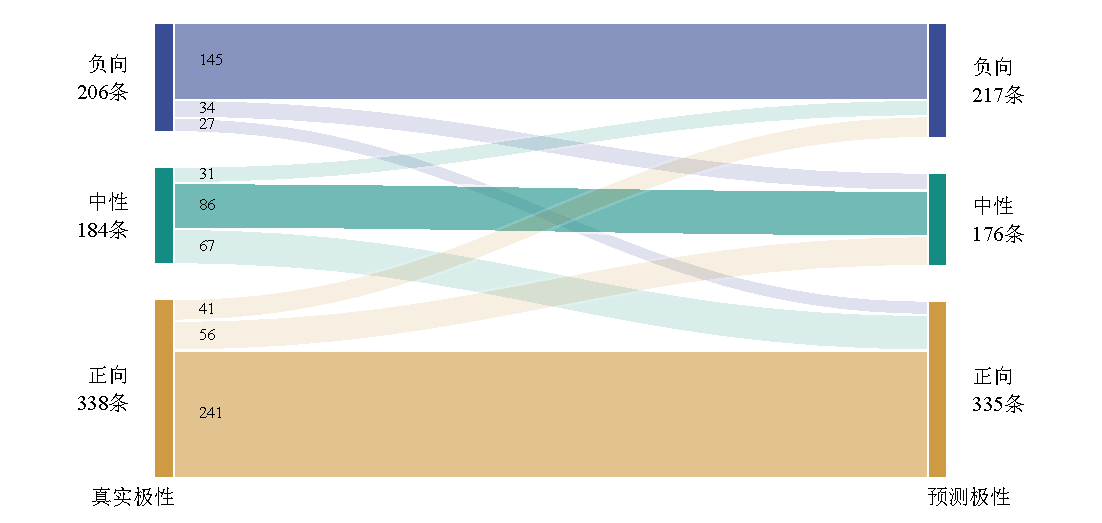
\includegraphics[width=.98\linewidth]{figures/极性预测流向.pdf}
 \caption{真实极性与预测极性的样本流向}
 \label{fig:p2-polarity-flow}
\end{figure}

\subsubsection*{（2）预测置信度可靠性}
图~\ref{fig:p2-reliability} 比较完整输入下预测类别的置信度与实际正确率。
按预测置信度划分十个等宽区间后，以每个非空区间的平均置信度和正确率作点，
误差棒表示正确率的Wilson 95\%区间\citep{wilson1927interval}，数字为各非空区间的样本数，
虚线表示置信度等于实际正确率。图中点大致沿理想对角线分布，
但部分区间存在偏差；低置信区间样本较少、区间较宽。
上述结果反映未经额外概率校准的模型在验证集上的置信度表现。
\begin{figure}[htbp]
 \centering
 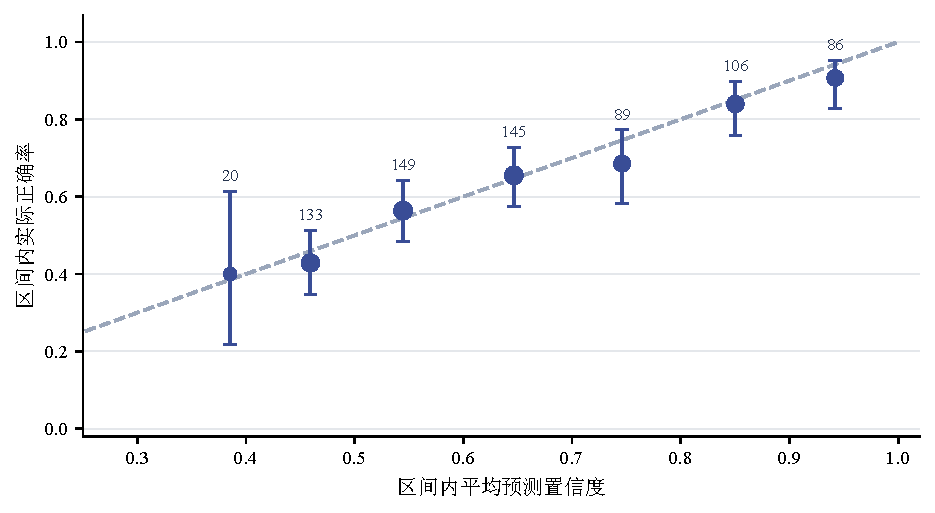
\includegraphics[width=0.98\linewidth]{figures/预测置信度可靠性.pdf}
 \caption{完整输入下的预测置信度可靠性}
 \label{fig:p2-reliability}
\end{figure}

\subsubsection*{（3）强度回归与符号投影}
原始回归输出的 MAE 和 Pearson 分别为 $0.5889$、$0.6504$；符号投影后分别为
$0.5769$、$0.6463$。投影使 MAE 改善 $0.0120$，但 Pearson 略降 $0.0041$。
这是因为中性预测被统一置零，正负类中符号冲突的输出被限制到对应半轴的近零边界，从而改变了绝对误差，
同时也压缩了部分预测变化范围。最终强度采用投影值，使其与预测极性的符号一致；
投影前后的指标共同反映这一约束对回归表现的影响。

图~\ref{fig:p2-strength-errors} 展示符号投影后强度预测的误差结构。
左图以真实强度为横轴、预测强度为纵轴，颜色对应真实极性，虚线表示理想预测。
右图将真实强度按单位区间分组，并将零值单独列出；圆点表示预测值减真实值的
残差中位数，粗线段表示第25至第75百分位，淡色轮廓展示各组残差的平滑分布，右列给出样本数。
轮廓厚度按各组峰值归一化，用于比较分布形状。
强负向区间 $[-3,-2)$ 与强正向区间 $(2,3]$ 的残差中位数分别为
$1.5813$ 和 $-1.4700$，对应 MAE 为 $1.6275$ 和 $1.6172$，表明两端预测均有向零收缩的倾向。
因此，总体 MAE 尚不能充分反映强情感样本的误差；但两端各仅有18条样本，
该现象的稳定性仍需更多样本验证。这一诊断描述最终输出的偏差，
训练分布、回归损失与符号投影各自的影响尚需进一步消融区分。
\begin{figure}[htbp]
 \centering
 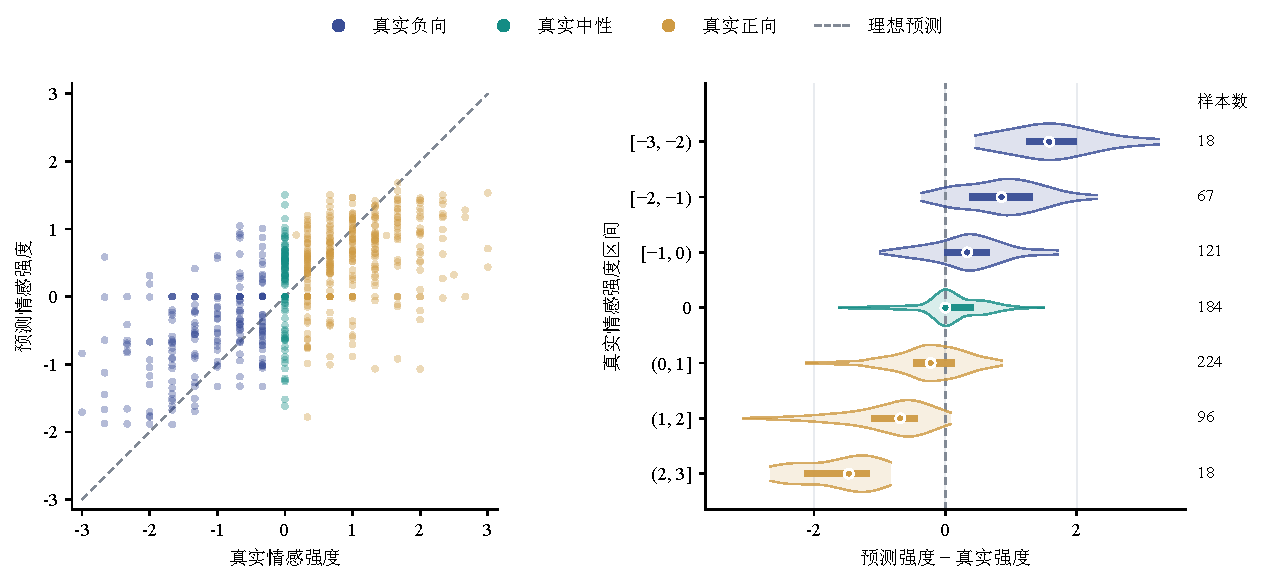
\includegraphics[width=.98\linewidth]{figures/情感强度预测与分区误差.pdf}
 \caption{情感强度预测与分区误差}
 \label{fig:p2-strength-errors}
\end{figure}

\subsubsection*{（4）训练与推理流程}

算法~\ref{alg:p2-training} 给出从一个批次的原始对齐特征到联合损失的完整步骤。
训练阶段的随机缺失只作用于训练集；验证阶段采用18种局部缺失场景及3种整模态移除场景；附件三
推理不再随机遮挡，只保留样本自身的观测掩码。

\begin{algorithm}[!htbp]
 \caption{观测掩码驱动的混合专家模型训练}
 \label{alg:p2-training}
 \setstretch{1.25}
 \begin{algorithmic}[1]
  \setlength{\itemsep}{4pt}
  \setlength{\parsep}{0pt}
  \AlgDescription $T$为文本词元序列，$\odot$为逐元素乘法，掩码沿特征维广播。
  $\operatorname{AvailabilityGate}$包含式~\eqref{eq:p2-gate-value}及模态不可用时的边界处理；
  $\mathcal L_{\rm rec}$按式~\eqref{eq:p2-reconstruction}仅在未遮挡文本子集上计算。
  \Require 批次 $\mathcal B=(T,A,V,M^{\rm str},M^x,M^a,M^v,c,y)$；参数 $\theta$
  \Ensure 更新后的参数 $\theta^{+}$
  \State $(D^x,D^a,D^v)\gets\operatorname{SampleMissing}(M^{\rm str},M^x,M^a,M^v)$
  \State $\widetilde M^q\gets M^q\odot(1-D^q),\quad q\in\{x,a,v\}$
  \State $\widetilde T\gets\operatorname{MaskTokens}(T,D^x)$
  \State $\widetilde A\gets A\odot\widetilde M^a,\quad\widetilde V\gets V\odot\widetilde M^v$
  \State $\boldsymbol z^x\gets\operatorname{TextExpert}(\operatorname{BERT}_{\rm frozen}(\widetilde T),\widetilde M^x)$
  \State $\boldsymbol r^{av}\gets\operatorname{AVExpert}(\widetilde A,\widetilde V,\widetilde M^a,\widetilde M^v)$
  \State $(\boldsymbol o^x,\hat y^x)\gets\operatorname{Heads}_x(\boldsymbol z^x),\quad
         (\boldsymbol o^{av},\hat y^{av})\gets\operatorname{Heads}_{av}(\boldsymbol r^{av})$
  \State $\rho^q\gets\frac{1}{50}\sum_t\widetilde M_t^q,\quad q\in\{x,a,v\}$
  \State $g\gets\operatorname{AvailabilityGate}(\boldsymbol z^x,\boldsymbol r^{av},\boldsymbol\rho)$
  \State $(\boldsymbol o,\hat y)\gets g(\boldsymbol o^x,\hat y^x)+(1-g)(\boldsymbol o^{av},\hat y^{av})$
  \State $\mathcal L\gets\mathcal L_{\rm cls}+0.2\mathcal L_{\rm reg}
         +0.2\mathcal L_x+0.3\mathcal L_{av}+0.02\mathcal L_{\rm rec}$
  \State $\theta^{+}\gets\operatorname{AdamW}(\theta,\nabla_\theta\mathcal L)$
 \end{algorithmic}
\end{algorithm}

模型选择依据完整输入和文本中部缺失40\%两种状态下的验证结果，
按式~\eqref{eq:p2-selection}确定各随机种子的最优轮次。
三种子集成对所选模型的输出取平均，不引入额外可训练参数。

\subsection{局部缺失鲁棒性分析}

\subsubsection{18种固定缺失场景}

图~\ref{fig:p2-text-position} 联合考察文本缺失位置、比例与预测任务。
左图横轴为Macro-F1、纵轴为投影后MAE，越靠右下表示两项表现越好；
三条箭头分别连接首部、中部和尾部缺失从20\%扩大至40\%的结果，菱形为完整输入。
右图展示相同场景的中性类别 F1，虚线对应完整输入。
尾部缺失扩大后，Macro-F1仅由0.5527变为0.5530，MAE却由0.6156升至0.6379；
其分类与回归响应并不一致。中性类别 F1在尾部缺失时虽由0.4011升至0.4113，
仍低于首部和中部场景。六场景的其余指标与音视频结果统一列于表~\ref{tab:p2-all-missing}。
\begin{figure}[htbp]
 \centering
 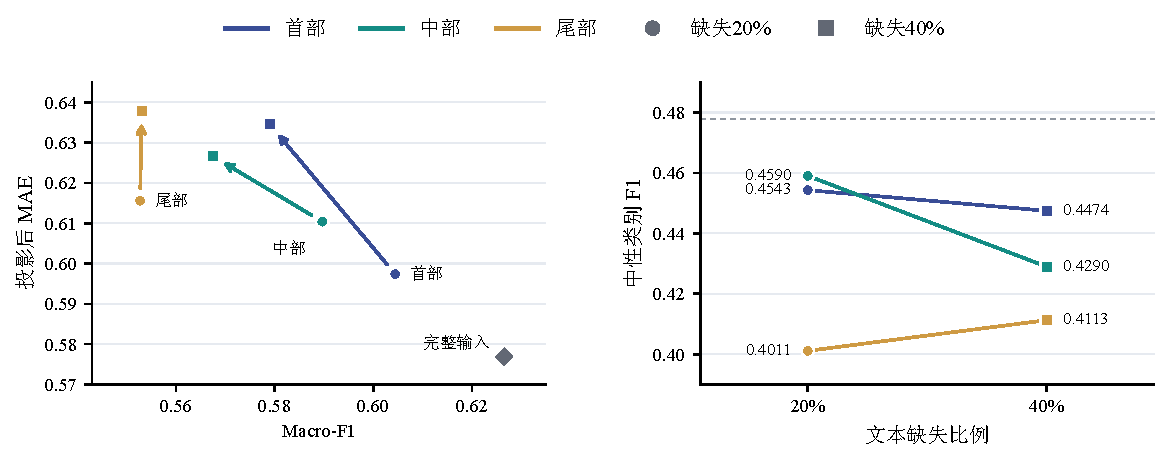
\includegraphics[width=.98\linewidth]{figures/文本缺失位置效应.pdf}
 \caption{文本缺失位置与比例对预测表现的影响}
 \label{fig:p2-text-position}
\end{figure}

\begin{table}[htbp]
 \centering
 \caption{最终模型在18种局部缺失场景下的完整结果}
 \label{tab:p2-all-missing}
 \begin{tabular*}{\linewidth}{@{\extracolsep{\fill}}cccccc@{}}
 \toprule
 模态 & 缺失设置 & ACC & Macro-F1 & 投影后MAE & 投影后Pearson \\
 \midrule
 文本 & 首部20\% & 0.6264 & 0.6044 & 0.5974 & 0.6207 \\
 文本 & 中部20\% & 0.6113 & 0.5896 & 0.6104 & 0.5850 \\
 文本 & 尾部20\% & 0.5755 & 0.5527 & 0.6156 & 0.5985 \\
 文本 & 首部40\% & 0.5975 & 0.5790 & 0.6345 & 0.5413 \\
 文本 & 中部40\% & 0.5907 & 0.5674 & 0.6267 & 0.5602 \\
 文本 & 尾部40\% & 0.5755 & 0.5530 & 0.6379 & 0.5667 \\
 \midrule
 语音 & 首部20\% & 0.6456 & 0.6243 & 0.5772 & 0.6466 \\
 语音 & 中部20\% & 0.6497 & 0.6285 & 0.5767 & 0.6463 \\
 语音 & 尾部20\% & 0.6484 & 0.6262 & 0.5775 & 0.6461 \\
 语音 & 首部40\% & 0.6456 & 0.6243 & 0.5778 & 0.6463 \\
 语音 & 中部40\% & 0.6456 & 0.6248 & 0.5777 & 0.6467 \\
 语音 & 尾部40\% & 0.6497 & 0.6281 & 0.5772 & 0.6465 \\
 \midrule
 视频 & 首部20\% & 0.6484 & 0.6268 & 0.5769 & 0.6462 \\
 视频 & 中部20\% & 0.6470 & 0.6262 & 0.5776 & 0.6459 \\
 视频 & 尾部20\% & 0.6470 & 0.6266 & 0.5779 & 0.6451 \\
 视频 & 首部40\% & 0.6497 & 0.6289 & 0.5764 & 0.6463 \\
 视频 & 中部40\% & 0.6470 & 0.6262 & 0.5773 & 0.6460 \\
 视频 & 尾部40\% & 0.6456 & 0.6259 & 0.5786 & 0.6448 \\
 \bottomrule
 \end{tabular*}
\end{table}

文本缺失对位置高度敏感。尾部缺失 $20\%$ 和 $40\%$ 的 Macro-F1 分别为
$0.5527$ 和 $0.5530$，均是六场景中的低值；首部 $20\%$ 仍为 $0.6044$。
该结果表明当前模型对验证样本的尾部文本缺失更敏感；具体原因还需结合语义内容与
片段长度进一步分析。缺失比例从 $20\%$
增加到 $40\%$ 时，首部和中部性能继续下降；尾部两种长度接近，表明较短尾部缺口已经
覆盖不少关键位置。

语音和视频局部缺失的波动明显小于文本；部分场景甚至略高于完整输入。小幅上升可能与音视频分支贡献较弱、局部噪声被遮挡或
有限验证集上的统计波动有关，现有实验尚未区分这些原因。结合音视频单独模型约 $0.40$ 的 Macro-F1 可知，
模型仍主要依赖文本，动态门控改善了文本局部缺失时的稳定性。

\subsubsection{整模态剔除与模型能力边界}

图~\ref{fig:p2-modality-removal} 比较固定三种子集成模型在输入移除后相对完整输入的
Macro-F1 变化，负值表示下降，正值表示提高。左图在统一尺度上展示三种模态，
左图阴影范围经直线连接到右侧同色放大区；右图单独展示语音和视频，两图纵轴尺度不同。
横轴为移除比例，20\%和40\%的点为首部、中部、尾部三种设置的均值，竖线表示最小值至最大值，
并非置信区间；全部移除时只有一种设置。水平虚线表示性能无变化。
文本移除的影响远大于语音或视频移除，显示最终模型仍明显依赖文本信息。
这些实验固定模型权重，仅剔除输入，用于刻画模态依赖，与重新训练的组件对照分别解释。
\begin{figure}[htbp]
 \centering
 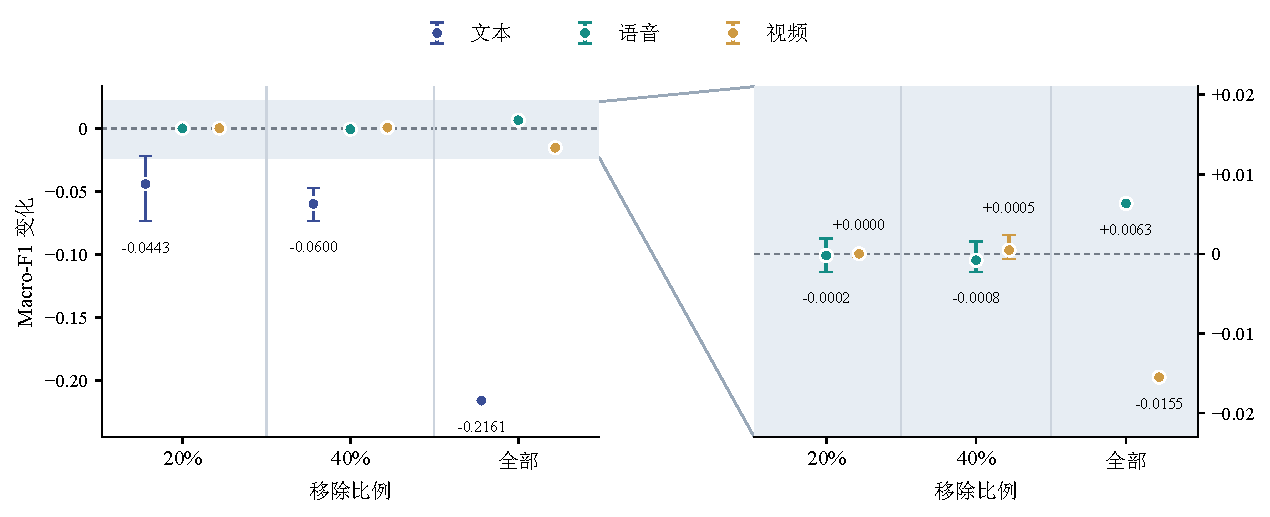
\includegraphics[width=0.98\linewidth]{figures/模态移除敏感性.pdf}
 \caption{局部缺失与整模态移除的性能变化}
 \label{fig:p2-modality-removal}
\end{figure}

完全移除文本时，ACC 为 $0.4299$、Macro-F1 为 $0.4104$、MAE 为 $0.7592$、
Pearson 为 $0.2683$。完全移除语音时 Macro-F1 为 $0.6329$，完全移除视频时为
$0.6110$。删除语音后略高于完整输入仍属于验证集现象，不代表语音在所有样本上有害；
问题三的逐样本贡献分析会进一步区分平均结果和个体差异。

完整输入时，中性和正向分别判对 $86/184$、$241/338$ 条；文本尾部缺失 $40\%$
后降为 $73/184$、$212/338$。这说明文本缺失同时伤害中性边界和正向语义识别。
全文本缺失时Macro-F1降至0.4104，音视频专家的补偿仍有限。
结合局部缺失实验，当前模型的主要收益体现在局部文本缺失时减缓性能退化。


\subsection{缺失条件下的专家融合行为}
\subsubsection*{（1）融合权重的样本分布}
为分析门控是否随观测条件变化，固定三个种子的网络参数，分别在完整输入、文本中部缺失、
音频中部缺失和视频中部缺失条件下计算728条验证样本的门控值。三种缺失条件均遮挡对应模态
40\%的观测位置，其余处理与前述鲁棒性实验一致。对样本 $s$，以三个模型门控值的均值
$\bar g_s=\frac13\sum_{k=1}^3g_s^{(k)}$ 汇总其文本专家权重。
该均值用于描述三个模型的共同趋势；实际集成仍分别计算各模型的预测，再平均分类logits和原始强度。

图~\ref{fig:p2-gate-cloud}以分布轮廓、样本散点及四分位区间展示不同条件下的 $\bar g_s$。
完整输入的均值为0.7481，中位数为0.7441，四分位区间为$[0.6913,0.8025]$，
表明模型总体较依赖文本，同时为音视频保留一定权重。
文本中部缺失后，均值降至0.7154，中位数降至0.7108；
音频和视频中部缺失时，均值分别为0.7459和0.7460，分布与完整输入较为接近。
局部音视频缺失后的分类表现也较稳定，与前述缺失实验呈现的文本依赖相一致。
\begin{figure}[htbp]
 \centering
 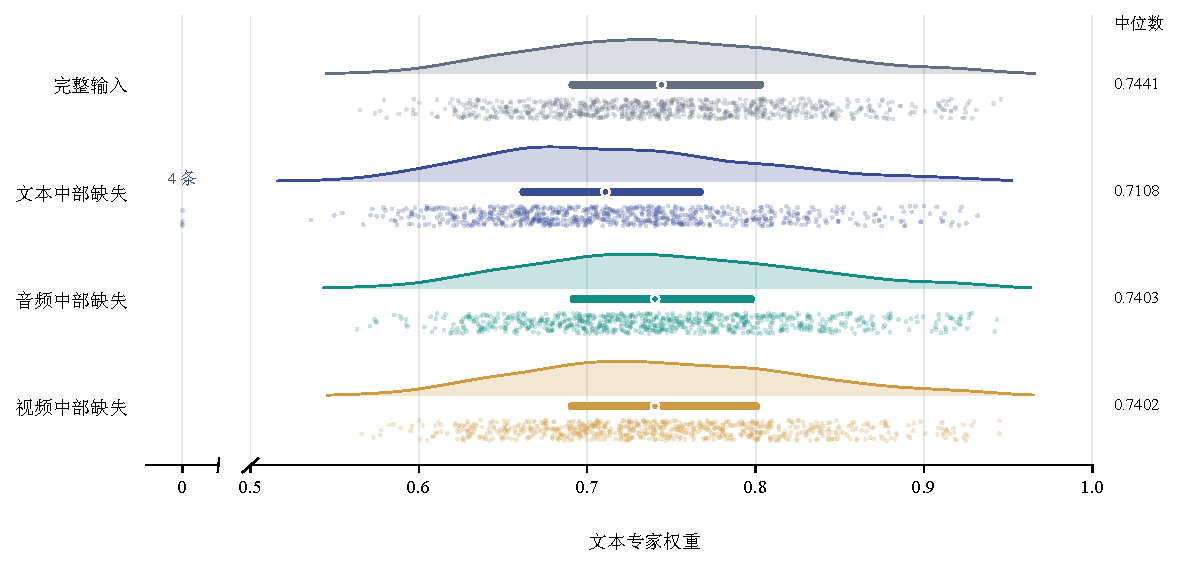
\includegraphics[width=.98\linewidth]{figures/缺失条件下的门控权重分布.pdf}
 \caption{完整输入与局部缺失条件下的文本专家权重分布}
 \label{fig:p2-gate-cloud}
\end{figure}

曲线为样本分布的平滑显示，散点表示逐样本权重，粗线段与圆点分别表示四分位区间和中位数。
横轴省略无样本的中间区间，保留零权重样本与主要分布。
各缺失场景使用相同样本，因此分布差异反映固定模型对输入变化的响应。
文本缺失场景中有4条样本的文本专家权重为零；按最少遮挡一个观测位置的规则，
极短文本可能在局部缺失实验中失去全部内容词元，从而触发确定性的音视频分支。
其余样本仍保留文本信息，采用连续门控进行融合。

\subsubsection*{（2）门控变化与预测变化的关系}
由式~\eqref{eq:p2-gate}，在两个专家的分类输出固定时，对文本门控的偏导为
\begin{equation}
 \frac{\partial\boldsymbol o_s}{\partial g_s}
 =\boldsymbol o_s^x-\boldsymbol o_s^{av}.
 \label{eq:p2-gate-sensitivity}
\end{equation}
因此，相同大小的门控变化在专家意见接近时影响较小，在专家明显分歧时影响较大。
实际遮挡会同时改变专家表示、专家输出和门控值，预测变化由这些因素共同决定。
尤其在文本部分缺失时，文本专家仍可能保留足够的语义证据，门控无需按缺失比例等幅下降；
音视频缺失也可能通过表示变化产生非单调响应。

文本中部40\%缺失时，最终Macro-F1为0.5674，较完整输入下降0.0591。
这一结果说明门控已发生适应性调整，但音视频提供的信息尚不足以完全补偿文本损失。
门控数值用于分析模型内部的融合行为，输入信息对最终判断的边际作用将在问题三通过遮挡与Shapley分解评价。

\subsection{随机种子稳定性与集成作用}

文本表征引导MoE三个单模型的完整 Macro-F1 分别为 $0.6188,0.6183,0.6295$，文本六场景
平均 Macro-F1 分别为 $0.5610,0.5792,0.5696$。不同种子在完整输入与文本缺失上的
排序并不一致，说明单模型的表现随随机种子变化。三种子集成后的完整 Macro-F1 为
$0.6265$，位于最佳单模型之下但高于三个单模型均值 $0.6222$；文本缺失平均值为
$0.5744$，高于三个单模型均值 $0.5699$。集成结果高于单模型的平均表现，但部分指标仍低于最优种子，
因此同时报告各单模型与集成结果。


三个种子分别采用第6、4、5轮的参数。各项指标并不总在同一轮达到最大值：
种子1的文本中部40\%缺失Macro-F1在第3轮为0.5665，高于第6轮的0.5472；
但第6轮完整输入表现与综合分数更优，因此按式~\eqref{eq:p2-selection}的综合准则采用第6轮。
这一差异体现了完整输入、缺失输入与强度回归目标之间的取舍。

种子1、2、3在最后记录轮次的综合分数分别为0.7159、0.7501和0.7222，
低于其采用轮次的0.7598、0.7687和0.7744，表明继续训练并未持续改善验证表现。
不同轨迹反映参数初始化、样本顺序及缺失增强的共同影响。由于只有三个随机种子，
这里报告实际波动和集成表现，不据此估计训练结果的总体置信区间。

模型集成先平均预测输出，再计算评价指标，因而与表~\ref{tab:p2-candidate-comparison}中的“三种子均值”具有不同含义。
以分类为例，logits平均改变了各类别之间的相对大小，可能纠正部分单模型错误，也可能改变原本正确的判断；
Macro-F1又由各类精确率与召回率非线性组合而成，其集成值不必等于单模型指标均值。
本实验中，完整输入指标未超过最佳种子，文本缺失六场景平均表现则较单模型均值有所改善，
因此集成的主要作用体现为综合不同训练结果，而非保证每个场景都优于全部单模型。


\subsection{附件三推理结果}

固定模型、集成规则及式~\eqref{eq:p2-sign-projection} 后，对附件三30条样本完成推理，
不再调整参数。负向、中性、正向预测
分别为 $7,7,16$ 条，强度范围为 $[-0.8773,1.2578]$，类别与强度符号逐条一致。
全部结果见表~\ref{tab:p2-attachment3}。
\begin{longtable}{@{\extracolsep{\fill}}cccccc@{}}
 \caption{附件三全部30条样本的极性与强度预测}\label{tab:p2-attachment3}\\
 \toprule
 编号 & 极性 & 强度 & 编号 & 极性 & 强度 \\
 \midrule
 \endfirsthead
 \multicolumn{6}{c}{表\thetable\ （续）}\\
 \toprule
 编号 & 极性 & 强度 & 编号 & 极性 & 强度 \\
 \midrule
 \endhead
 \bottomrule
 \endfoot
01 & 负向 & -0.4489 & 16 & 正向 & 1.2578 \\
02 & 中性 & 0.0000 & 17 & 负向 & -0.1185 \\
03 & 中性 & 0.0000 & 18 & 正向 & 0.5381 \\
04 & 正向 & 0.4683 & 19 & 负向 & -0.3557 \\
05 & 负向 & -0.8773 & 20 & 中性 & 0.0000 \\
06 & 正向 & 0.8321 & 21 & 正向 & 0.6385 \\
07 & 正向 & 0.6429 & 22 & 正向 & 0.2715 \\
08 & 负向 & -0.1653 & 23 & 中性 & 0.0000 \\
09 & 正向 & 1.0187 & 24 & 负向 & -0.2105 \\
10 & 中性 & 0.0000 & 25 & 中性 & 0.0000 \\
11 & 正向 & 0.2327 & 26 & 正向 & 0.6681 \\
12 & 正向 & 0.3280 & 27 & 正向 & 0.6932 \\
13 & 正向 & 0.6038 & 28 & 正向 & 0.5884 \\
14 & 负向 & -0.6748 & 29 & 正向 & 0.4176 \\
15 & 正向 & 0.7790 & 30 & 中性 & 0.0000 \\
\end{longtable}


附件三未提供真实标签，其预测误差无法直接估计。模型性能由附件二验证集评价，
附件三的类别分布与强度范围用于描述专项样本的预测结果。

\subsection{本问小结}

本问在附件二对齐版上建立了观测掩码驱动的混合专家模型。通过区分结构有效、自然
未观测和人工连续缺失，模型能够采用统一的输入表示处理完整输入和局部缺失；冻结 BERT 文本
专家、掩码卷积音视频专家、分支监督与动态门控共同构成预测主干，辅助重构只作为小权重
训练约束。三种子集成在完整输入的验证集上取得 ACC $0.6484$、Macro-F1 $0.6265$、投影后
MAE $0.5769$ 和 Pearson $0.6463$。文本六个局部缺失场景平均 Macro-F1 为
$0.5744$，完全移除文本时降至 $0.4104$，表明局部鲁棒性有所改善而文本依赖仍是主要
限制。固定模型已完成附件三全部 $30$ 条样本的极性与强度输出。

% ==================== problem3
\section{问题三：模态贡献与局部证据解释}
\label{sec:problem3}

廖勇等\citep{liao2026xai}从解释模型、解释方法、安全测试与实验验证四个方面梳理
可解释人工智能技术。本文将解释与预测模型的实际响应联系起来，分别检验模态贡献的
加和关系和局部证据的遮挡敏感性。

图~\ref{fig:p3-explanation-flow} 概括预测解释的计算过程。模态贡献通过八种保留组合的输出差异计算，
局部证据通过逐模态滑窗遮挡确定；随后选取主要参考模态的高响应窗口，记录其原文及媒体来源。
文本词元可映射到原文，音视频窗口与原素材的时间对应取决于可获得的时间信息。
\begin{figure}[htbp]
 \centering
 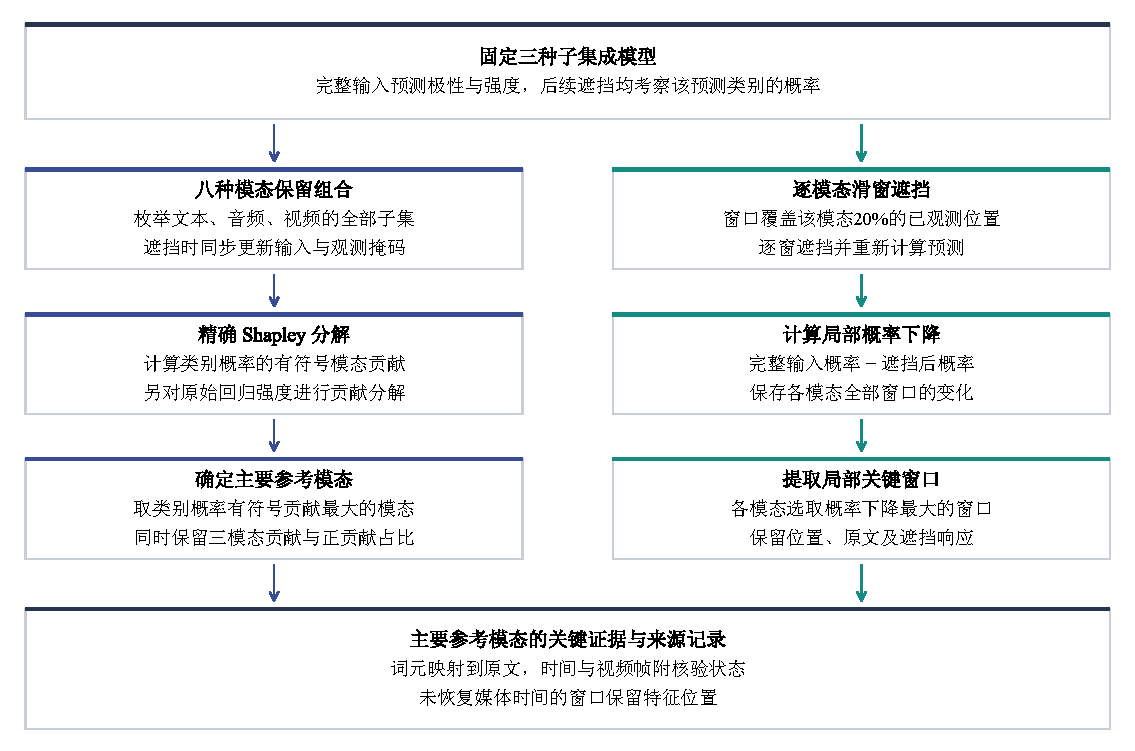
\includegraphics[width=.98\linewidth]{figures/预测解释流程.pdf}
 \caption{模态贡献与局部证据的计算流程}
 \label{fig:p3-explanation-flow}
\end{figure}

\subsection{共享预测模型与模态贡献}
问题三沿用问题二已固定的文本表征引导MoE三种子集成及对齐版输入，不另用附件四
调整参数、阈值或解释规则。其网络结构、联合目标和训练参数见第~\ref{sec:problem2}~节。
解释阶段固定模型权重，基础预测性能与问题二相同：验证集ACC为0.6484、Macro-F1为0.6265，
投影后MAE为0.5769、Pearson为0.6463；中性识别与强情感向零收缩是主要误差来源。
本节进一步按真实类别和预测正确性分析解释结果。对每条完整输入的预测类别 $c^\ast$，
采用Shapley加性归因思想\citep{shap2017}，把文本、语音、视频视为三个参与者。令 $v(S)$ 为仅保留模态集合
$S\subseteq\{x,a,v\}$ 时模型赋给 $c^\ast$ 的概率；被移除模态的
观测掩码与数值同时清除，文本词元改为 \texttt{[MASK]}。
计算全部 $2^3=8$ 个组合，再按 Shapley 公式
\begin{equation}
 \phi_q=\sum_{S\subseteq M\setminus\{q\}}
 \frac{|S|!(|M|-|S|-1)!}{|M|!}
 \left[v(S\cup\{q\})-v(S)\right],\quad M=\{x,a,v\}.
 \label{eq:p3-shapley}
\end{equation}
因此 $\sum_q\phi_q=v(M)-v(\varnothing)$。另对原始回归强度
按上式计算贡献。$\phi_q$ 可为负，表示该模态在组合平均意义下
压低当前预测类别概率；展示用的非负占比定义为
$\max(\phi_q,0)/\sum_j\max(\phi_j,0)$，分母为零时全设为零。
极性主模态取概率贡献中最大有符号 $\phi_q$，强度主模态取原始回归贡献的绝对值最大者。
下文未特别说明的“主要参考模态”均指极性主模态；门控值本身不充当解释。
空输入基线是三模态均被遮挡后的模型输出，不解释为现实中的
“没有情感”视频。

计算时固定完整输入上的预测类别 $c^\ast$，对每个模态子集 $S$，只读取模型对
同一类别 $c^\ast$ 的概率，而不在每个子集上重新挑选目标类别。简写
$v(xa)=v(\{x,a\})$ 等，则文本模态的三人 Shapley 贡献可展开为
\begin{equation}
\begin{aligned}
 \phi_x={}&\frac13[v(x)-v(\varnothing)]
 +\frac16[v(xa)-v(a)] +\frac16[v(xv)-v(v)]\\
 &+\frac13[v(xav)-v(av)],
\end{aligned}
\label{eq:p3-shapley-expanded}
\end{equation}
语音和视频贡献按对称方式计算。由于参与者数只有 $3$，每条样本只需精确评估
$8$ 种输入组合，不使用随机排列近似。每次移除模态时，同时清除对应数值与观测掩码；
文本内容词元改为 \texttt{[MASK]} 后重新运行冻结编码器，避免沿用含有被删词上下文的
预计算双向表示。强度贡献以符号投影前的原始回归输出为价值函数，按相同的边际差公式计算。

按 Shapley 的可加性规则，三个有符号贡献之和等于完整输入相对全遮挡输入的输出差；
该性质用于检验贡献计算的数值一致性。贡献值表示模型在给定输入和遮挡方式下的响应，
不保证反事实输入符合真实自然分布，也不证明某个词、音调或表情在现实中造成了情绪。
正贡献占比只在解释“支持当前类别的正向分量”时使用；如果存在负贡献，它不等于
有符号总差的比例。门控系数、注意力权重和 Shapley 值分别是模型融合参数、内部权重
和输出反事实贡献，三者不可互换。

表~\ref{tab:p3-global-shapley} 汇总728条验证样本的模态贡献。视频模态有15条样本无有效观测，
其贡献为零，因此正、负贡献的计数以其余713条为分母；平均贡献仍按全部728条计算。
每条样本将有符号贡献 $\phi$ 最大的模态记为主要参考模态，并统计其出现次数。

\begin{table}[htbp]
 \centering
 \caption{验证集全模态 Shapley 概率贡献的描述统计}
 \label{tab:p3-global-shapley}
 \begin{tabular*}{\linewidth}{@{\extracolsep{\fill}}ccccc@{}}
 \toprule
 模态 & 平均有符号$\phi$ & $\phi>0$条数 & $\phi<0$条数 & 最大有符号贡献模态次数 \\
 \midrule
 文本 & 0.3176 & 698/728 & 30/728 & 632/728 \\
 语音 & 0.0068 & 413/728 & 315/728 & 54/728 \\
 视频 & 0.0204 & 428/713 & 285/713 & 42/728 \\
 \bottomrule
 \end{tabular*}
\end{table}


图~\ref{fig:p3-shapley-distribution} 展示按预测类别分组的逐样本有符号贡献。
每个点代表附件二验证集的一条样本，短黑线为组内中位数，横向虚线为零贡献；
散点表明均值之外仍有明显的样本差异。

\begin{figure}[htbp]
 \centering
 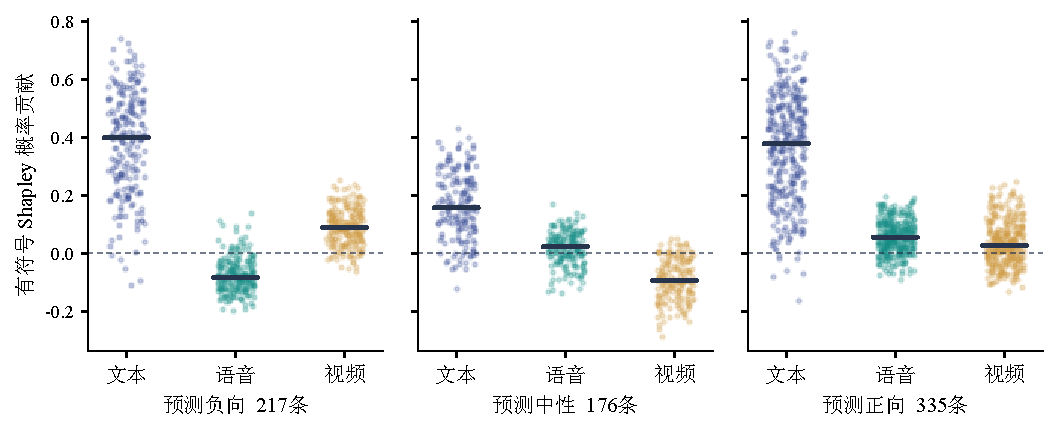
\includegraphics[width=0.98\linewidth]{figures/预测类别模态贡献分布.pdf}
 \caption{按预测类别分组的三模态 Shapley 贡献分布}
 \label{fig:p3-shapley-distribution}
\end{figure}

为检查文本主导现象是否只由某一类标签造成，表~\ref{tab:p3-shapley-strata}
按真实类别分层。各行中的 $\phi$ 仍解释模型对完整输入预测类别 $c^\ast$ 的概率，
而不是对真实标签概率的归因；“主模态”是逐样本最大有符号贡献的频数。
三类中文本均为最常见主模态，说明本模型在验证集上的文本依赖广泛存在于不同极性样本中。

\begin{table}[htbp]
 \centering
 \caption{按真实极性分层的验证集模态贡献}
 \label{tab:p3-shapley-strata}
 \setlength{\tabcolsep}{3pt}
 \begin{tabular*}{\linewidth}{@{\extracolsep{\fill}}cccccccc@{}}
 \toprule
 真实类别 & 样本数 & 平均$\phi_x$ & 平均$\phi_a$ & 平均$\phi_v$ & 主模态文本 & 主模态语音 & 主模态视频 \\
 \midrule
 负向 & 206 & 0.3524 & $-0.0471$ & 0.0412 & 181 & 11 & 14 \\
 中性 & 184 & 0.2359 & 0.0188 & $-0.0153$ & 160 & 16 & 8 \\
 正向 & 338 & 0.3409 & 0.0331 & 0.0271 & 291 & 27 & 20 \\
 \bottomrule
 \end{tabular*}
\end{table}

\subsection{局部证据与忠实度检查}
遮挡敏感性通过移除局部输入并比较模型输出来定位重要区域\citep{zeiler2014occlusion}。
本文将这一思路用于多模态序列，在每个模态的实际观测位置上，以观测数的 $20\%$ 为连续窗口宽度
逐位置滑动并逐段遮挡。对候选窗口 $I$ 定义
$d_q(I)=p_{c^\ast}(\boldsymbol x)-p_{c^\ast}(\boldsymbol x\setminus I)$，取 $d_q$ 最大的窗口为关键证据，
同时记录最低分与固定随机窗口，分别作为低敏感度和随机选窗的参照。
本文另设宽窗口复核：以选出窗口的中心为基准扩大到
$40\%$ 宽度，重新计算预测类别概率下降。令模态 $q$ 有 $L_q$ 个观测位置，
候选窗口长度为 $w_q=\max\{1,\operatorname{round}(0.2L_q)\}$；将观测位置按原序排列，
在该序列上滑动形成候选窗 $I_{q,j}$。定义
\begin{equation}
 d_q(I_{q,j})=p_{c^\ast}(\boldsymbol x)-
 p_{c^\ast}(\boldsymbol x\setminus I_{q,j}),\qquad
 I_q^{\rm high}=\arg\max_jd_q(I_{q,j}),\quad
 I_q^{\rm low}=\arg\min_jd_q(I_{q,j}).
 \label{eq:p3-local-drop}
\end{equation}
随机基线由固定随机种子按样本与模态确定，因此重复运行选到同一窗口。$d_q$ 为正表示
遮挡使当前预测类别概率降低；为负则表示遮挡后概率反而上升。由于窗口宽度按各自模态
观测位置数定义，文本词元位置、音频对齐位置和视频对齐位置并不代表相同的实际秒数。

图~\ref{fig:p3-text-window-map} 用验证集索引 $0$--$29$ 的连续 $30$ 条样本展示文本
候选窗口扫描。色标采用以零为中心、正负对称的线性映射。
正值表示遮挡后当前预测类别概率下降，负值表示概率上升；灰色为该样本
没有对应候选窗口的位置。横轴只表示每条样本自身的候选窗口次序，跨行同一序号
不代表同一个词或相同时间。该图用于展示局部响应的差异，定量忠实度仍由全体
$728$ 条样本的宽窗口复核给出。
\begin{figure}[htbp]
 \centering
 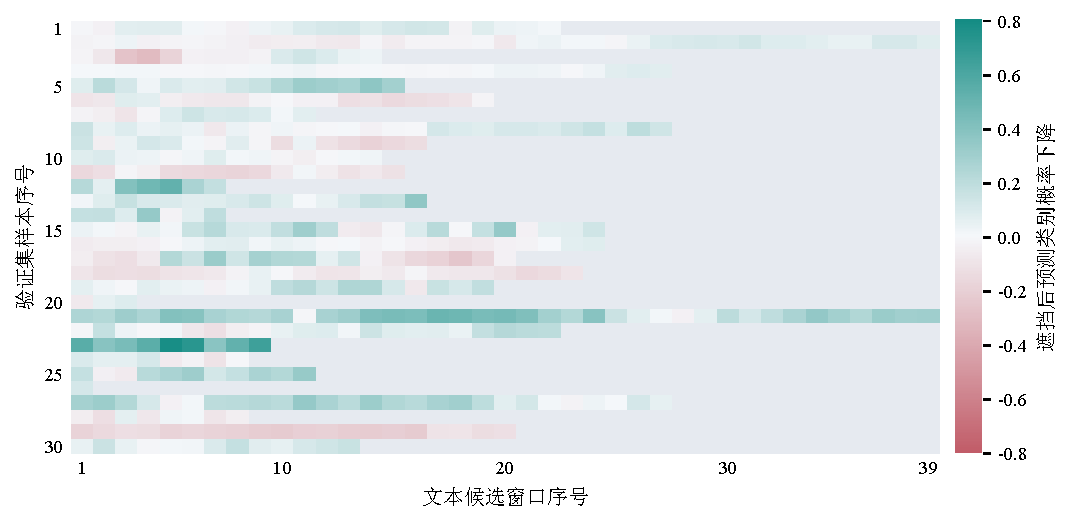
\includegraphics[width=0.98\linewidth]{figures/文本局部窗口响应.pdf}
 \caption{连续30条验证样本的文本局部遮挡响应}
 \label{fig:p3-text-window-map}
\end{figure}

解释规则固定后，在附件二全部728条验证样本上作宽窗口复核。
图~\ref{fig:p3-local-fidelity} 中每个点对应一条样本，横、纵轴分别为随机窗和高分窗
遮挡后的预测类别概率下降；窗口均由20\%宽度选点后扩大到40\%。
点在对角虚线上方表示高分窗的影响大于随机窗，文本、语音和视频的这一比例分别为
67.86\%、72.12\%和74.33\%。视频仅统计713条有观测样本；三个子图各自使用等比例坐标，
轴范围不同，跨模态比较应依据数值。每个子图上方展示随机窗响应的边际分布，右侧展示高分窗响应的边际分布，
平滑轮廓用于辅助观察各自的集中程度。文本散点分布较宽，说明平均优势仍伴随个体不稳定性。
\begin{figure}[htbp]
 \centering
 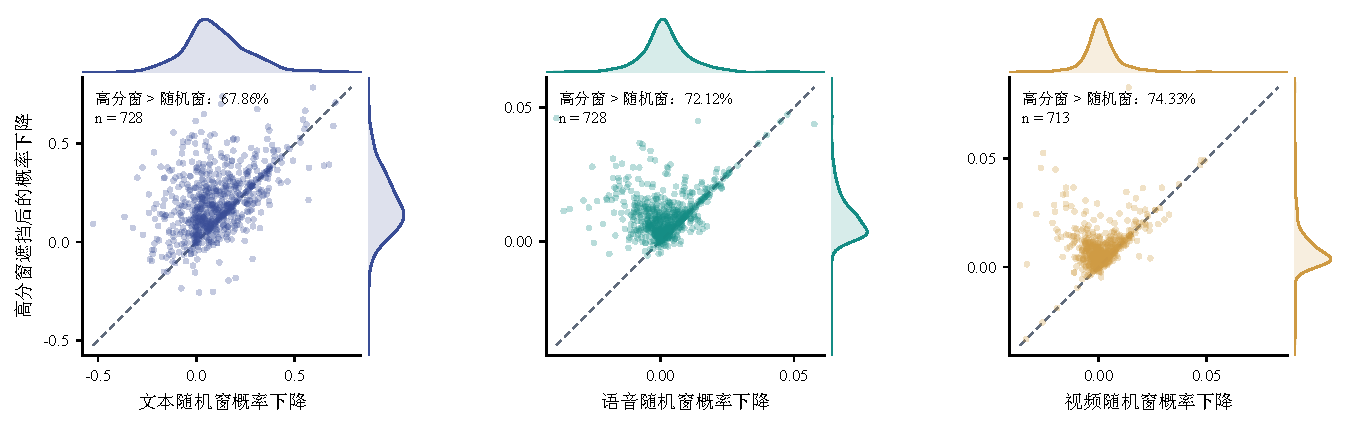
\includegraphics[width=.98\linewidth]{figures/局部解释忠实度散点.pdf}
 \caption{宽窗口复核下的逐样本局部解释忠实度}
 \label{fig:p3-local-fidelity}
\end{figure}

作为均值补充，文本高分、随机和低分窗口的概率下降依次为0.1954、0.0994和0.0256；
语音依次为0.0088、0.0019和$-0.0060$，视频为0.0075、0.0015和$-0.0050$。
音视频窗口影响的绝对幅度明显较小；高分窗胜过随机窗的比例更高，也不表示其影响更大。
这些统计均来自参与模型选择的开发验证集。

按真实类别与预测正确性拆分后，同一 $40\%$ 宽窗口复核仍呈现明显的组间差异，
见表~\ref{tab:p3-local-strata}。三种真实类别中，文本高分窗平均下降均高于随机窗，
但“高分大于随机”的比例为 $0.6576$--$0.6893$；总体均值不能掩盖个体不稳定性。
错误样本也可能对文本遮挡敏感，故该检验衡量解释窗口对模型输出的忠实度，
而非模型是否识别正确。

\begin{table}[htbp]
 \centering
 \caption{按标签和预测正确性分层的文本宽窗口忠实度}
 \label{tab:p3-local-strata}
 \begin{tabular*}{\linewidth}{@{\extracolsep{\fill}}ccccc@{}}
 \toprule
 样本分组 & 数量 & 高分窗平均下降 & 随机窗平均下降 & 高分大于随机比例 \\
 \midrule
 真实负向 & 206 & 0.2029 & 0.0889 & 0.6893 \\
 真实中性 & 184 & 0.1657 & 0.0898 & 0.6576 \\
 真实正向 & 338 & 0.2069 & 0.1110 & 0.6834 \\
 预测正确 & 472 & 0.2075 & 0.1082 & 0.6716 \\
 预测错误 & 256 & 0.1730 & 0.0831 & 0.6914 \\
 \bottomrule
 \end{tabular*}
\end{table}

\subsection{解释方法的验证集评价}
模态贡献与局部敏感性回答模型依据了哪些输入，预测正确性则由输出类别与真实标签的比较确定。
本节使用附件二带真实标签的728条验证样本，将预测类别与真实极性逐条比较，
得到472条预测正确样本和256条预测错误样本，
比较其文本Shapley贡献与宽窗口复核结果。采用经验累积分布展示全部样本，
横轴给出响应数值，纵轴给出不超过该数值的样本比例，避免仅用组均值概括分布差异。

定义文本宽窗口的配对响应差为
\begin{equation}
 \Delta_s=d_x(\widetilde I_s^{\rm high})-d_x(\widetilde I_s^{\rm random}),
 \label{eq:p3-paired-gain}
\end{equation}
其中两个窗口均由20\%窗口确定中心后扩大至40\%，与前文复核设置一致。
同一样本的完整预测概率在两项相减时抵消，因此 $\Delta_s$ 直接比较两种遮挡后的目标类别概率；
$\Delta_s>0$ 表示高分窗的影响大于随机窗。
这一比较保留了逐样本配对关系，避免将某些样本原本较高的置信度误当作窗口选择优势。
\begin{figure}[htbp]
 \centering
 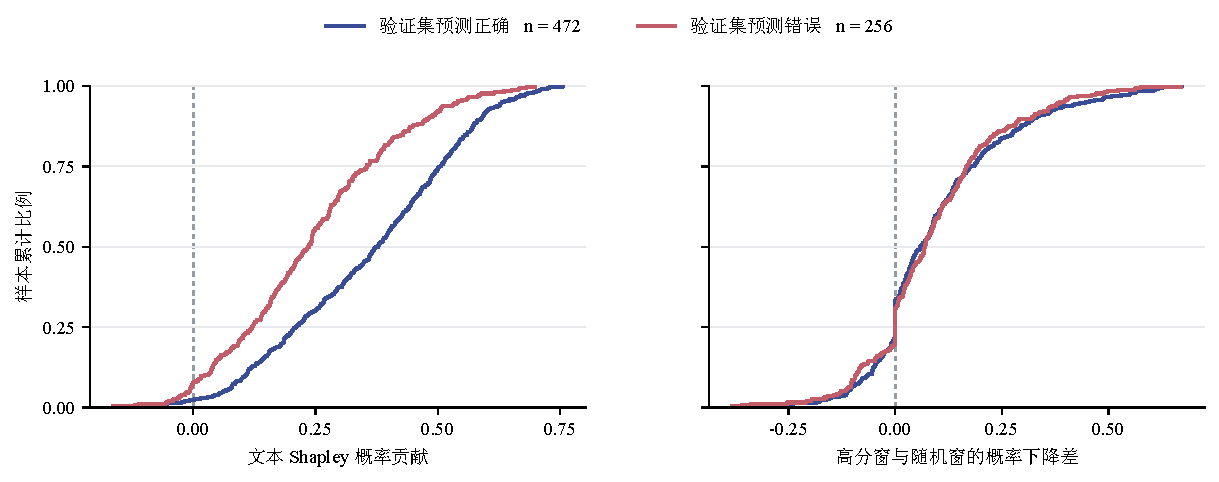
\includegraphics[width=.98\linewidth]{figures/预测正确性与解释响应分布.pdf}
 \caption{验证集正确与错误预测的文本贡献及局部响应分布}
 \label{fig:p3-correctness-response}
\end{figure}

图~\ref{fig:p3-correctness-response}左图显示，正确组的文本贡献整体偏大：中位数为0.3756，
错误组为0.2355。但错误组中仍有237条样本的文本贡献为正，占256条的92.58\%。
这说明文本也可能支持与真实标签不一致的模型判断。
正贡献只表示提高当前预测类别的概率，其符号并不评价该类别是否正确。

右图中两组配对响应差的分布高度重叠。正确组和错误组的均值分别为0.0993和0.0899，
中位数分别为0.0586和0.0689；高分窗优于随机窗的样本分别为317条和177条。
错误组的中位数并未更小，说明解释窗口对模型的影响强弱不足以单独区分正确与错误预测。
这一现象也补充了表~\ref{tab:p3-local-strata}的均值结果：两组均存在有影响力的文本片段，
但模型对这些片段所作的类别判断可能不同于真实标签。

因此，解释评价需要同时关注预测表现和响应忠实性。若预测正确且高分窗有明显影响，
可以进一步检查其对应语义是否与判断一致；若预测错误但响应明显，应重点分析模型是否过度依赖局部词语、
忽略上下文或混淆中性边界。这些是后续误差分析的方向，具体成因仍需结合原文逐例判断。
附件四缺少真实标签，其贡献值与局部响应用于分析预测依据。

\FloatBarrier
\subsection{附件四预测、证据与原视频回溯}
\subsubsection*{（1）预测分布与证据覆盖}
固定上述方法后，对附件四20条样本输出极性、强度、三模态有符号贡献、
正贡献占比、主要参考模态和关键证据位置。
20 条结果中负／中／正预测数为 $8/4/8$，主要参考模态为
文本 $19$ 条、视频 $1$ 条。附件四未提供真实标签，预测误差无法由该组数据估计。
完整结果见表~\ref{tab:p3-attachment4}。
这些计数用于描述本组样本的预测与解释分布。

\begin{table}[htbp]
 \centering
 \caption{附件四预测分布与解释证据覆盖}
 \label{tab:p3-output-audit}
 \begin{tabularx}{\linewidth}{@{}ccY@{}}
 \toprule
 项目 & 结果 & 说明 \\
 \midrule
 样本覆盖 & 20/20 & 全部样本均获得预测与解释结果 \\
 文本词元一致性 & 20/20 & 原文重新分词所得序列与输入BERT词元一致 \\
 Shapley可加性检查 & 20/20 & 三模态贡献之和等于完整与全遮挡概率差，容差$10^{-6}$ \\
 类别输出 & 负8、中4、正8 & 附件四无真实标签，仅报告预测计数 \\
 最大贡献模态 & 文本19、视频1 & 按每条样本最大有符号Shapley值确定 \\
 文本时间候选 & 7/20 & 目标文本基本位于候选区间内 \\
 视频帧时间候选 & 1条 & 05号样本的邻近画面与目标话语对应 \\
 \bottomrule
 \end{tabularx}
\end{table}

\subsubsection*{（2）关键证据与原视频回溯}
附件四本身未给对齐特征位置的真实秒数映射。文本位置先与
文件内原转写重新词元化核对，20 条的 BERT 词元序列均逐项匹配；
再用各自视频的 16\,kHz 音轨、冻结的wav2vec 2.0字符级CTC声学模型\citep{wav2vec2020}与原转写
求词时间候选。仅当自由解码与原文字符相似度不低于 $0.90$、
证据区间每个词的平均字符置信度不低于 $0.50$ 且时间落在
音频范围内时，才填写候选秒数。7 条文本证据通过此自动筛查，
经试听，这7条证据的目标文本基本位于候选区间内，逐词边界误差尚未量化。
其余证据定位至特征序列位置；
对齐特征索引与原视频秒数之间未建立线性映射。
编号 05 利用相应文本的候选时段，在自身视频中选取显示时刻为
$1.733$ 秒的邻近候选帧。经视频回看，该帧与所选话语附近画面一致；
视频特征位置与帧时间的精确对应尚缺乏独立标注。
上述试听和回看用于核查展示内容与原素材的对应关系，未据此修改情感预测、模态贡献或算法选取的关键窗口。
例如编号 01 的文本关键位置 $7$--$10$ 对应
 \emph{the timing belt is}，候选音频时间为 $2.620$--$3.660$ 秒；
编号 03 的位置 $17$--$23$ 对应
 \emph{who don't take rental income}，候选为 $4.100$--$5.760$ 秒。
这些区间表示模型敏感片段的自动时间估计。

\subsubsection*{（3）典型样本的贡献与局部敏感性}
图~\ref{fig:p3-cases} 联合展示三个典型样本的模态贡献与局部敏感性。
编号 01 的最高文本窗概率下降为 $0.1329$，但随机窗也下降 $0.1181$，两者差距有限；
编号 03 的高分文本窗下降 $0.2603$，随机窗却略有上升，局部敏感性更集中。
编号 05 的全模态视频贡献最大，但视频局部高分窗只改变 $0.0199$；同时文本局部窗
变化为 $0.2309$。这表明“某模态整体贡献最大”不能直接推出“其单个时间段最关键”。
三个例子的局部敏感性均在特征序列上计算，CTC 时间与邻近视频帧用于辅助定位。

图~\ref{fig:p3-cases} 展示编号 01、03、05 的模态贡献与
各自主要模态的局部遮挡曲线。左侧为三模态有符号贡献，右侧为主要模态的连续窗口
遮挡结果，空心菱形与竖直虚线标出所选局部窗口，邻近数值为其概率下降。
中间的模态贡献共用横轴范围；右侧三行依次展示文本、文本、视频窗口，纵轴范围各自标明。
窗口横轴为候选次序，不代表视频秒数。
编号 05 的文本局部高分窗口为位置1--3。

\begin{figure}[htbp]
 \centering
 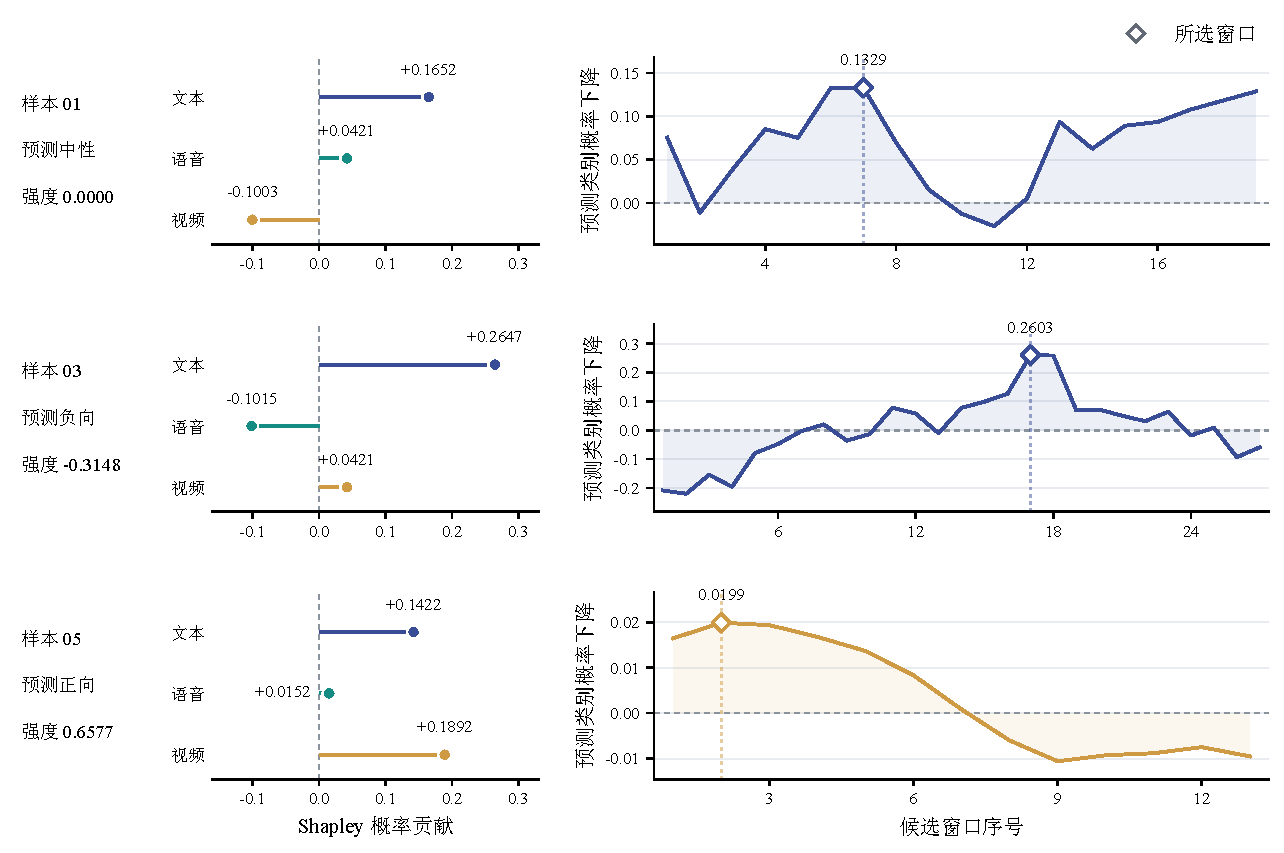
\includegraphics[width=\linewidth]{figures/解释样本.pdf}
 \caption{附件四典型样本的模态贡献与局部遮挡响应}
 \label{fig:p3-cases}
\end{figure}

\subsection{附件四20条样本预测与主要证据}
表~\ref{tab:p3-attachment4} 汇总预测结果、主要参考模态及三模态贡献占比。
预测概率 $p^*=p_{c^*}$ 为完整输入下预测类别 $c^*$ 的概率。
极性主模态取该类别概率的有符号Shapley贡献最大者；强度主模态取原始回归输出的
绝对Shapley贡献最大者，表示对回归输出影响幅度最大的模态。
强度列给出符号投影后的最终预测，强度主模态解释投影前的回归输出，因此中性预测也可有强度主模态。
三个占比均由极性概率的正贡献归一化得到，极性与强度的有符号贡献明细分别见附录表~\ref{tab:appendix-contributions}和表~\ref{tab:appendix-strength-contributions}。
19号样本的强度落在负向投影边界$-10^{-6}$，表中保留科学计数形式，以区别于中性零值。

% Generated by src/q3_explanation/export_paper_tables.py
\begingroup
\setlength{\tabcolsep}{3pt}
\begin{longtable}{@{\extracolsep{\fill}}ccccccccc@{}}
\caption{附件四全部样本的预测与模态贡献}\label{tab:p3-attachment4}\\
\toprule
\multirow{2}{*}{编号} & \multirow{2}{*}{极性} & \multirow{2}{*}{强度} & \multirow{2}{*}{预测概率} & \multirow{2}{*}{\makecell[c]{极性\\主模态}} & \multirow{2}{*}{\makecell[c]{强度\\主模态}} & \multicolumn{3}{c}{极性正贡献占比/\%} \\
\cmidrule(lr){7-9}
 & & & & & & 文本 & 音频 & 视频 \\
\midrule
\endfirsthead
\multicolumn{9}{c}{表 \thetable\ （续）}\\
\toprule
\multirow{2}{*}{编号} & \multirow{2}{*}{极性} & \multirow{2}{*}{强度} & \multirow{2}{*}{预测概率} & \multirow{2}{*}{\makecell[c]{极性\\主模态}} & \multirow{2}{*}{\makecell[c]{强度\\主模态}} & \multicolumn{3}{c}{极性正贡献占比/\%} \\
\cmidrule(lr){7-9}
 & & & & & & 文本 & 音频 & 视频 \\
\midrule
\endhead
\bottomrule
\endfoot
01 & 中性 & 0.0000 & 0.5763 & 文本 & 音频 & 79.69 & 20.31 & 0.00 \\
02 & 正向 & 0.1739 & 0.3999 & 文本 & 文本 & 75.32 & 0.00 & 24.68 \\
03 & 负向 & -0.3148 & 0.5355 & 文本 & 文本 & 86.26 & 0.00 & 13.74 \\
04 & 负向 & -0.3423 & 0.6942 & 文本 & 文本 & 100.00 & 0.00 & 0.00 \\
05 & 正向 & 0.6577 & 0.6014 & 视频 & 文本 & 41.02 & 4.40 & 54.58 \\
06 & 正向 & 0.7153 & 0.7590 & 文本 & 文本 & 100.00 & 0.00 & 0.00 \\
07 & 正向 & 0.9381 & 0.7685 & 文本 & 文本 & 69.48 & 8.86 & 21.66 \\
08 & 正向 & 0.7534 & 0.6986 & 文本 & 文本 & 100.00 & 0.00 & 0.00 \\
09 & 负向 & -1.8113 & 0.9787 & 文本 & 文本 & 83.05 & 5.15 & 11.80 \\
10 & 负向 & -1.4535 & 0.9603 & 文本 & 文本 & 97.21 & 0.00 & 2.79 \\
11 & 负向 & -0.3506 & 0.6287 & 文本 & 文本 & 69.96 & 0.00 & 30.04 \\
12 & 负向 & -0.9411 & 0.8439 & 文本 & 文本 & 95.03 & 0.00 & 4.97 \\
13 & 中性 & 0.0000 & 0.6059 & 文本 & 文本 & 71.74 & 28.26 & 0.00 \\
14 & 中性 & 0.0000 & 0.6554 & 文本 & 视频 & 89.98 & 10.02 & 0.00 \\
15 & 正向 & 1.2534 & 0.9308 & 文本 & 文本 & 71.86 & 16.82 & 11.33 \\
16 & 负向 & -1.7715 & 0.9777 & 文本 & 文本 & 96.81 & 0.00 & 3.19 \\
17 & 正向 & 1.3957 & 0.9487 & 文本 & 文本 & 82.70 & 3.01 & 14.29 \\
18 & 中性 & 0.0000 & 0.4925 & 文本 & 文本 & 100.00 & 0.00 & 0.00 \\
19 & 负向 & $-1\times10^{-6}$ & 0.5501 & 文本 & 音频 & 77.16 & 0.00 & 22.84 \\
20 & 正向 & 0.9360 & 0.8436 & 文本 & 文本 & 77.67 & 3.54 & 18.80 \\
\end{longtable}
\endgroup


表~\ref{tab:p3-attachment4-evidence} 列出极性主模态的关键证据，特征位置采用对齐版输入的零基索引。
文本行给出对应原文及可用的CTC时间估计，05号展示约1.733秒的邻近候选画面。
右列分别给出文本时间区间或视频候选帧时刻，空缺时保留特征位置。

% Generated by src/q3_explanation/export_paper_tables.py
\begingroup
\setlength{\tabcolsep}{3pt}
\begin{longtable}{@{\extracolsep{\fill}}cccC{76mm}c@{}}
\caption{附件四全部样本的关键证据与对应位置}\label{tab:p3-attachment4-evidence}\\
\toprule
编号 & 模态 & 特征位置 & 关键原文或候选画面 & \mbox{时间区间或时刻/s} \\
\midrule
\endfirsthead
\multicolumn{5}{c}{表 \thetable\ （续）}\\
\toprule
编号 & 模态 & 特征位置 & 关键原文或候选画面 & \mbox{时间区间或时刻/s} \\
\midrule
\endhead
\bottomrule
\endfoot
01 & 文本 & 7--10 & the timing belt is & [2.620, 3.660] \\
02 & 文本 & 9--12 & other’s happiness - not & -- \\
03 & 文本 & 17--23 & who don't take rental income & [4.100, 5.760] \\
04 & 文本 & 21--25 & goodbye?] Absolutely not. & [4.480, 6.240] \\
05 & 视频 & 2--4 & \raisebox{\dimexpr-.5\height+.5ex\relax}{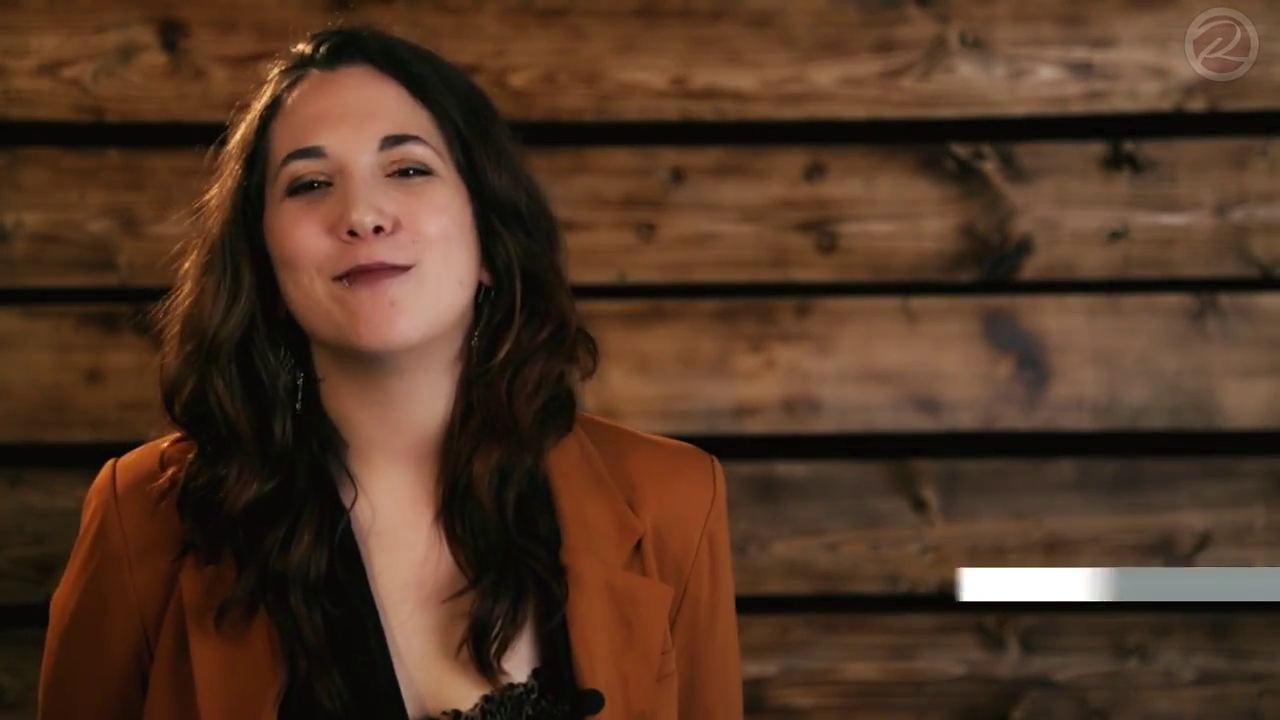
\includegraphics[height=18mm]{../outputs/q3_explanation/q3/visual_candidate_05.png}} & 1.733 \\
06 & 文本 & 1--7 & If you're a fan of & -- \\
07 & 文本 & 21--30 & enthusiastically discussed the topics of growing the hobby, the & -- \\
08 & 文本 & 2--3 & brings us & [0.860, 1.180] \\
09 & 文本 & 7--10 & not like this movie & -- \\
10 & 文本 & 12--17 & see fluffy chick flicks sometimes & [2.880, 4.960] \\
11 & 文本 & 2--4 & would be ashamed & -- \\
12 & 文本 & 34--41 & sag, and credit scores is very low. & -- \\
13 & 文本 & 23--28 & two of the given factors or & -- \\
14 & 文本 & 21--27 & Uniform Final Examination (UFE) & -- \\
15 & 文本 & 5--8 & poverty, the family & -- \\
16 & 文本 & 9--10 & a terrible & -- \\
17 & 文本 & 10--14 & simple, easy and will & [4.800, 6.940] \\
18 & 文本 & 3--12 & in Denmark - the first Baltic Cod fishery has been & -- \\
19 & 文本 & 12--19 & mistakes, and unfortunately some haters out & [3.900, 6.900] \\
20 & 文本 & 19--27 & we'll have more live updates and a & -- \\
\end{longtable}
\endgroup



\subsection{解释可靠性与使用边界}
问题三从模态贡献的加和关系、局部证据的跨尺度敏感性和原素材对应关系三个层次评价解释结果。
表~\ref{tab:p3-claim-boundary}汇总各项验证结果及其适用范围。

\begin{table}[htbp]
 \centering
 \caption{解释方法的验证结果与适用范围}
 \label{tab:p3-claim-boundary}
 \begin{tabularx}{\linewidth}{@{}cC{50mm}Y@{}}
 \toprule
 验证内容 & 实测结果 & 适用范围 \\
 \midrule
 全局模态分解 & 三模态8组合精确枚举；验证集728条加和误差均小于$10^{-6}$ & 三种贡献之和等于完整输入与全遮挡的概率差；不表示模态对现实情绪的因果效应 \\
 局部窗口迁移 & 20\%选窗后用40\%窗口复核；文本高分窗优于随机窗比例0.6786 & 文本片段在平均意义上更敏感；该排序在约三分之一验证样本上未胜过随机窗 \\
 词元—原文核对 & 附件四20条词元序列均与原文一致 & 可复核关键特征位置与文本内容；不能仅凭一致性得到词的真实发音时间 \\
 秒级证据定位 & 7条文本CTC候选、1条视频帧候选 & 可回溯部分证据的原始内容；精确定位误差尚未量化 \\
 验证与专项样本 & 验证集472/728预测正确；附件四20条无标签 & 验证结果反映模型在开发数据上的表现；附件四缺少用于评价预测误差的真实标签 \\
 \bottomrule
 \end{tabularx}
\end{table}

综上，模态贡献与局部遮挡共同描述固定模型对输入变化的响应。特征位置的定位
由遮挡窗口确定，媒体时间则来自额外的自动对齐，两者具有不同的精度来源。
现有实验支持特征层面的敏感性分析，秒级定位精度和证据的情绪语义仍有待独立评估。

% ==================== evaluation
\section{模型评价与展望}
\label{sec:evaluation}
本文分别建立原始素材的特征对齐流程，以及标准化特征上的预测与解释流程。结合第~\ref{sec:problem1}~至第~\ref{sec:problem3}~节的实验，
从方法优势、适用局限与后续改进三个方面作如下评价。

\subsection{模型优点}
\begin{enumerate}
 \item \textbf{时间与观测信息保留完整。}
 特征提取采用词时间戳与原生区间交叠建立对应，并分别保留结构有效掩码和模态观测掩码，
 使序列填充、未检出人脸与真实观测具有不同含义。100条样本均保留特征来源与质量记录，
 词级表示与原生观测通过时间区间及来源索引关联，能够将数据质量问题定位到具体模态和时间区间。

 \item \textbf{完整输入与局部缺失采用同一预测框架。}
 混合专家模型结合文本语义和音视频时序表示，并利用观测比例调整融合权重。
 连续片段遮挡训练与确定性缺失评估使用一致的掩码语义，便于比较不同位置、时长和
 模态缺失下的表现。最终模型完整输入Macro-F1为$0.6265$，文本六种局部缺失场景的
 平均Macro-F1为$0.5744$；相对统计融合与回归混合方案，二者分别提高$0.0174$和$0.0125$，
 表明当前验证条件下完整预测与局部鲁棒性能够同时改善。

 \item \textbf{模态贡献与局部证据具有明确的计算定义。}
 三模态仅有八种组合，可以精确枚举Shapley贡献并检查加和关系；局部证据通过遮挡后
 的类别概率变化衡量，再以更宽窗口复核。模态贡献、局部敏感性与原视频候选位置形成
 分层证据，使解释能够对应到实际模型响应。分类与回归同时报告，并保留符号投影前后
 的指标，也便于识别不同评价目标之间的取舍。
\end{enumerate}

\subsection{模型局限}
\begin{enumerate}
 \item \textbf{细粒度对齐仍受原始素材质量限制。}
 80条样本中的1533个词取得可用时间，其中1374个取得三模态特征。
 20条因音文不一致、其他语言或无对应语音而保留原生序列；另48条样本共有103个词位置未取得可用时间。
 单脸筛选减少多人混合，仍不能保证所有帧中检测到的脸就是当前说话人。
 附件一自提取特征与附件二预处理特征的定义也存在差异，当前结果尚未验证两者之间
 可直接迁移同一预测模型。

 \item \textbf{文本依赖与类别、强度误差仍然明显。}
 完全移除文本时Macro-F1降至$0.4104$，说明音视频专家的补偿能力有限；
 中性类别F1为$0.4778$，低于正负类别。强情感区间的预测还呈现向零收缩，
 总体MAE会掩盖部分极端样本误差。符号投影改善MAE的同时略微降低Pearson，
 表明输出一致性与连续强度拟合之间仍有取舍。

 \item \textbf{泛化与组件收益的证据范围有限。}
 候选比较、超参数和轮次选择反复使用同一验证集，所报告的改进可能偏乐观。
 文本表征引导MoE相对基础MoE的集成增益较小，各种子指标的均值也未呈现一致的缺失鲁棒性收益，
 尚需更多重复实验判断稳定性。现有压力测试主要覆盖单模态连续缺失及整模态移除，
 对多模态同时缺失、零散缺失和实际噪声干扰的结论仍不充分。附件三、四没有标签，
 无法据此估计专项预测误差。

 \item \textbf{遮挡解释依赖基线与扰动方式。}
 全遮挡基线、窗口宽度和替换方式均可能影响贡献值，遮挡还可能产生偏离自然输入的
 组合。扩大窗口后的验证支持文本高分片段在平均意义上较敏感，但个体排序仍会变化。
 因此，当前解释适用于描述固定模型的输入敏感性，其现实情绪含义还需独立证据支持。
\end{enumerate}

\subsection{未来展望}
\begin{enumerate}
 \item \textbf{完善时间对齐与质量分层。}
 进一步完善低置信词的边界估计及音视频特征位置到原始素材的时间映射。
 在具有可靠人工边界的样本上评估词时间误差与来源覆盖率，再扩大细粒度对齐范围。
 若进一步连接自提取特征与预测模型，应先统一特征定义与标准化规则，单独验证跨来源
 表示差异对预测的影响。

 \item \textbf{围绕已定位的短板改进预测与验证。}
 后续可在附件二训练集内部设计分层交叉验证，将方案选择与效果估计分开，
 并报告不同种子和划分下的波动。模型改进优先围绕音视频独立判别能力、中性边界及
 强情感样本展开，比较分支监督、采样策略与回归损失的实际收益；同时补充多模态联合
 缺失和噪声测试。所有新增方案均应在开发数据上固定后再进行专项推理。

 \item \textbf{评估解释稳定性与推理成本。}
 后续可比较不同遮挡基线、窗口尺度及随机重复下的证据排序，结合独立标注的时间
边界和内容判定，检验关键片段是否稳定且可定位。三种子集成和逐窗口解释需要多次
 模型前向计算，还应实测延迟与资源占用；在保持预测和解释质量的前提下，再评估
 单模型蒸馏、候选窗口筛选等简化方案。上述方向均需新增实验验证其收益。
\end{enumerate}

\section*{人工智能工具使用说明}
\addcontentsline{toc}{section}{人工智能工具使用说明}
本研究过程中使用DeepSeek V4.1 Flash\citep{deepseek2026flash}与
GPT-6 Astra\citep{openai2026astra}辅助文献检索、论文排版、
代码整理与修复、绘图脚本编写和修改，以及复现材料整理。
相关辅助涉及Python代码和
LaTeX文本；实验数值来自赛题数据与程序输出，引用信息按文献原文和出版方记录核对。
相关代码与排版修改经代码检查、结果比对和排版检查复核。

\FloatBarrier
\Needspace{6\baselineskip}
\bibliographystyle{gmcm-numerical}
\bibliography{reference}


% Code excerpts follow the repository implementation; see docs/论文维护说明.md.
\clearpage
\appendix
\renewcommand{\theHsection}{appendix.\Alph{section}}
\renewcommand{\thesubsection}{\Alph{section}.\arabic{subsection}}
\renewcommand{\thetable}{\Alph{section}.\arabic{table}}
\definecolor{codeKeyword}{HTML}{225EA8}
\definecolor{codeString}{HTML}{98613D}
\definecolor{codeComment}{HTML}{557368}
\lstset{language=Python,basicstyle=\small\ttfamily\linespread{1.05}\selectfont,
 keywordstyle=\color{codeKeyword},commentstyle=\color{codeComment},stringstyle=\color{codeString},
 frame=single,rulecolor=\color{black!30},breaklines=true,breakatwhitespace=true,
 columns=fullflexible,keepspaces=true,showstringspaces=false,tabsize=4,
 aboveskip=8pt,belowskip=8pt}
\BeforeBeginEnvironment{lstlisting}{\Needspace{5\baselineskip}}
\section{补充结果与复现材料}
\label{sec:appendix-reproduction}

\subsection{问题一：特征维度与典型样本对应}
\subsubsection*{（1）声学与面部特征的维度定义}
文本表示为冻结BERT的768维末层向量。声学特征的列序、计算含义和可用条件见表~\ref{tab:appendix-audio-dimensions}；
13个MFCC与四个声学量共同组成17维表示。表中列序从1开始，数组索引从0开始。
静音窗仍保留声学特征，基频不可测时仅将该维的观测掩码置为假；
词级基频汇聚仅使用可测窗，并重新归一化交叠权重。
\begin{table}[htbp]
\centering
\caption{17维声学特征的排列与有效性}\label{tab:appendix-audio-dimensions}
\begin{tblr}{width=\linewidth,colspec={c c c X[c] X[c]},cells={valign=m,font=\normalsize\songti},
 colsep=4pt,rowsep=3pt,hline{1,7}={0.8pt},hline{2}={0.4pt}}
列序号 & 特征 & 维数 & 定义 & 可用条件 \\
1--13 & MFCC $c_0$--$c_{12}$ & 13 & 26通道对数mel谱的前13个正交倒谱系数 & 存在完整声学窗 \\
14 & 对数RMS & 1 & 去均值波形均方根幅值的自然对数 & 存在完整声学窗 \\
15 & 基频/Hz & 1 & 60--400 Hz内自相关峰值对应频率 & 峰值至少0.30，RMS至少$10^{-3}$ \\
16 & 频谱质心/Hz & 1 & 幅值谱的频率加权均值 & 完整声学窗；全零谱取零 \\
17 & 过零率 & 1 & 相邻采样点符号变化次数除以399 & 存在完整声学窗 \\
\end{tblr}
\end{table}


面部系数按英文名称排序，分组与列序见表~\ref{tab:appendix-video-dimensions}。
这些系数描述面部形变，其中基准系数\texttt{\_neutral}不代表情感分类中的中性概率。
词级面部特征仅汇聚单脸有效帧。电子结果中的特征维度表列出全部17个声学量与52个面部系数的名称、索引和掩码，
与每份特征文件内的名称序列一致。
\begin{table}[htbp]
\centering
\caption{52维面部系数的分组与排列}\label{tab:appendix-video-dimensions}
\begin{tabular*}{\linewidth}{@{\extracolsep{\fill}}ccc@{}}
\toprule
列序号 & 系数组 & 维数 \\
\midrule
1 & 基准系数 & 1 \\
2--6 & 眉部 & 5 \\
7--9 & 面颊 & 3 \\
10--23 & 眼部 & 14 \\
24--27 & 下颌 & 4 \\
28--50 & 口部 & 23 \\
51--52 & 鼻部 & 2 \\
\bottomrule
\end{tabular*}
\end{table}

\FloatBarrier

\subsubsection*{（2）典型样本逐词对应}
样本片段\texttt{-egA8-b7-3M\_9}的10个词均通过词时间筛查。
表~\ref{tab:appendix-word-times} 给出自动时间与交叠来源数量；试听确认内容及大致位置，
没有单独标注精确起止边界。
\begin{table}[htbp]
\centering
\caption{典型样本词时间与来源数量}\label{tab:appendix-word-times}
\begin{tabular*}{\linewidth}{@{\extracolsep{\fill}}ccccc@{}}
\toprule
序号 & 单词 & 时间区间/s & 语音窗数 & 视频帧数\\\midrule
1 & Secondly, & $[0.560, 1.040)$ & 51 & 16 \\
2 & another & $[1.260, 1.620)$ & 38 & 12 \\
3 & goal & $[1.680, 1.880)$ & 23 & 7 \\
4 & of & $[1.960, 2.000)$ & 6 & 2 \\
5 & exhibiting & $[2.100, 2.580)$ & 51 & 15 \\
6 & is & $[2.740, 2.800)$ & 9 & 2 \\
7 & building & $[2.900, 3.280)$ & 41 & 12 \\
8 & your & $[3.320, 3.460)$ & 16 & 5 \\
9 & company & $[3.520, 3.900)$ & 40 & 12 \\
10 & image. & $[4.040, 4.300)$ & 28 & 8 \\
\bottomrule
\end{tabular*}
\end{table}

\subsection{问题二：模型组件与逐类表现}
\subsubsection*{（1）候选模型的组件配置}
表~\ref{tab:appendix-model-components}列出统一训练器中六类候选的结构与辅助目标，
与正文表~\ref{tab:p2-candidate-comparison}的对应模型名称一致。

含文本的候选均采用冻结BERT，音视频卷积与BiLSTM候选仅使用音视频输入；
各模型均有极性分类与强度回归目标，回归项权重为0.2。
表中分支监督系数作用于相应分支的分类与回归联合损失。
跨模态注意力使用两层、四头、128维编码；MoE的两个专家输出通过样本级门控融合。
种子1、2、3依次为2026、2027、2028，各模型的训练轮次独立按验证集综合分数选择。
这些候选涉及编码结构、融合方式或辅助目标的变化，比较范围以表中配置为准。

\begin{table}[htbp]
\centering
\caption{候选模型的结构与辅助目标}\label{tab:appendix-model-components}
\begin{tblr}{width=\linewidth,colspec={X[1.4,c] X[1.1,c] X[1.2,c] X[1.2,c] X[1.2,c] c},
 cells={valign=m,font=\normalsize\songti},colsep=3pt,rowsep=2pt,hline{1,8}={0.8pt},hline{2}={0.4pt}}
模型 & 音视频编码 & 融合方式 & 分支监督 & 辅助约束 & 种子 \\
音视频卷积 & \makecell[c]{64维\\残差卷积} & 拼接与MLP & 无 & 无 & 1 \\
\makecell[c]{音视频\\BiLSTM} & 双向LSTM & 拼接与MLP & 无 & 无 & 1 \\
\makecell[c]{掩码跨模态\\注意力} & \makecell[c]{64维\\残差卷积} & \makecell[c]{两层跨模态\\注意力} & 无 & 无 & 1 \\
基础MoE & \makecell[c]{64维\\残差卷积} & 双专家门控 & \makecell[c]{文本0.2\\音视频0.3} & 无 & 1、2、3 \\
中性辅助MoE & \makecell[c]{64维\\残差卷积} & 双专家门控 & \makecell[c]{文本0.2\\音视频0.3} & \makecell[c]{中性二元\\损失0.3} & 1、2 \\
\makecell[c]{文本表征引导\\MoE} & \makecell[c]{64维\\残差卷积} & 双专家门控 & \makecell[c]{文本0.2\\音视频0.3} & \makecell[c]{文本重构\\0.02} & 1、2、3 \\
\end{tblr}
\end{table}

\FloatBarrier

\subsubsection*{（2）完整输入与缺失场景的逐类指标}
正文采用ACC、Macro-F1和回归指标比较缺失场景；表~\ref{tab:appendix-class-f1}
补充完整输入及21种缺失场景的逐类F1与加权F1。所有结果来自同一固定集成模型和728条验证样本。
\begingroup
\renewcommand{\arraystretch}{1.25}
\begin{longtable}{@{\extracolsep{\fill}}ccccccc@{}}
\caption{完整输入与缺失场景的逐类F1}\label{tab:appendix-class-f1}\\
\toprule
缺失模态 & 比例 & 位置 & 负向F1 & 中性F1 & 正向F1 & 加权F1 \\
\midrule
\endfirsthead
\multicolumn{7}{c}{表\thetable\ （续）}\\
\toprule
缺失模态 & 比例 & 位置 & 负向F1 & 中性F1 & 正向F1 & 加权F1 \\
\midrule
\endhead
\bottomrule
\endfoot
完整 & -- & -- & $0.6856$ & $0.4778$ & $0.7162$ & $0.6473$ \\
文本 & 20\% & 首部 & $0.6579$ & $0.4543$ & $0.7011$ & $0.6265$ \\
文本 & 20\% & 中部 & $0.6223$ & $0.4590$ & $0.6876$ & $0.6114$ \\
文本 & 20\% & 尾部 & $0.6049$ & $0.4011$ & $0.6522$ & $0.5753$ \\
文本 & 40\% & 首部 & $0.6208$ & $0.4474$ & $0.6688$ & $0.5993$ \\
文本 & 40\% & 中部 & $0.6047$ & $0.4290$ & $0.6687$ & $0.5900$ \\
文本 & 40\% & 尾部 & $0.5996$ & $0.4113$ & $0.6483$ & $0.5746$ \\
文本 & 100\% & 全部 & $0.3850$ & $0.3123$ & $0.5340$ & $0.4358$ \\
语音 & 20\% & 首部 & $0.6840$ & $0.4765$ & $0.7124$ & $0.6447$ \\
语音 & 20\% & 中部 & $0.6872$ & $0.4820$ & $0.7162$ & $0.6488$ \\
语音 & 20\% & 尾部 & $0.6825$ & $0.4791$ & $0.7170$ & $0.6471$ \\
语音 & 40\% & 首部 & $0.6840$ & $0.4765$ & $0.7124$ & $0.6447$ \\
语音 & 40\% & 中部 & $0.6841$ & $0.4780$ & $0.7124$ & $0.6451$ \\
语音 & 40\% & 尾部 & $0.6825$ & $0.4847$ & $0.7170$ & $0.6485$ \\
语音 & 100\% & 全部 & $0.6975$ & $0.4903$ & $0.7108$ & $0.6513$ \\
视频 & 20\% & 首部 & $0.6825$ & $0.4807$ & $0.7173$ & $0.6476$ \\
视频 & 20\% & 中部 & $0.6857$ & $0.4807$ & $0.7122$ & $0.6462$ \\
视频 & 20\% & 尾部 & $0.6824$ & $0.4848$ & $0.7126$ & $0.6465$ \\
视频 & 40\% & 首部 & $0.6857$ & $0.4848$ & $0.7162$ & $0.6491$ \\
视频 & 40\% & 中部 & $0.6857$ & $0.4807$ & $0.7122$ & $0.6462$ \\
视频 & 40\% & 尾部 & $0.6792$ & $0.4877$ & $0.7106$ & $0.6454$ \\
视频 & 100\% & 全部 & $0.6634$ & $0.4736$ & $0.6962$ & $0.6306$ \\
\end{longtable}
\endgroup

\subsection{问题三：模态贡献与局部证据}
\subsubsection*{（1）极性概率贡献}
表~\ref{tab:appendix-contributions} 补充附件四全部20条样本的有符号Shapley贡献。
贡献针对各样本完整输入的预测类别计算，正值表示提高该类别概率，负值表示降低；
三模态之和等于完整输入与全遮挡输入的概率差。数值保留四位小数。
\begingroup
\renewcommand{\arraystretch}{1.25}
\begin{longtable}{@{\extracolsep{\fill}}ccccc@{}}
\caption{附件四全部样本的三模态贡献}\label{tab:appendix-contributions}\\
\toprule
编号 & 文本贡献 & 语音贡献 & 视频贡献 & 极性主模态 \\
\midrule
\endfirsthead
\multicolumn{5}{c}{表\thetable\ （续）}\\
\toprule
编号 & 文本贡献 & 语音贡献 & 视频贡献 & 极性主模态 \\
\midrule
\endhead
\bottomrule
\endfoot
01 & $0.1652$ & $0.0421$ & $-0.1003$ & 文本 \\
02 & $0.1711$ & $-0.0794$ & $0.0561$ & 文本 \\
03 & $0.2647$ & $-0.1015$ & $0.0421$ & 文本 \\
04 & $0.5303$ & $-0.0892$ & $-0.0444$ & 文本 \\
05 & $0.1422$ & $0.0152$ & $0.1892$ & 视频 \\
06 & $0.5870$ & $-0.0262$ & $-0.0482$ & 文本 \\
07 & $0.3776$ & $0.0481$ & $0.1177$ & 文本 \\
08 & $0.5085$ & $-0.0670$ & $-0.0093$ & 文本 \\
09 & $0.5833$ & $0.0362$ & $0.0829$ & 文本 \\
10 & $0.6612$ & $-0.0445$ & $0.0190$ & 文本 \\
11 & $0.2944$ & $-0.0623$ & $0.1264$ & 文本 \\
12 & $0.5900$ & $-0.1390$ & $0.0308$ & 文本 \\
13 & $0.1220$ & $0.0481$ & $0.0000$ & 文本 \\
14 & $0.4113$ & $0.0458$ & $-0.2255$ & 文本 \\
15 & $0.4889$ & $0.1144$ & $0.0771$ & 文本 \\
16 & $0.7318$ & $-0.0585$ & $0.0241$ & 文本 \\
17 & $0.5789$ & $0.0210$ & $0.1000$ & 文本 \\
18 & $0.1601$ & $-0.0499$ & $-0.0108$ & 文本 \\
19 & $0.2497$ & $-0.1123$ & $0.0739$ & 文本 \\
20 & $0.4820$ & $0.0219$ & $0.1167$ & 文本 \\
\end{longtable}
\endgroup


\subsubsection*{（2）情感强度贡献}
表~\ref{tab:appendix-strength-contributions}给出符号投影前原始回归输出的Shapley贡献。
正值表示该模态提高原始强度，负值表示降低原始强度；强度主模态按贡献绝对值最大者确定。
其方向与数值均针对连续回归输出。预测为负向时，负贡献也可能增强模型的负向判断；
贡献绝对值描述影响幅度。中性样本的最终强度经投影置零，其原始回归贡献仍可非零。
% Generated by src/q3_explanation/export_paper_tables.py
\begingroup
\setlength{\tabcolsep}{3pt}
\begin{longtable}{@{\extracolsep{\fill}}ccccc@{}}
\caption{附件四全部样本的原始强度贡献}\label{tab:appendix-strength-contributions}\\
\toprule
编号 & 文本贡献 & 音频贡献 & 视频贡献 & 强度主模态 \\
\midrule
\endfirsthead
\multicolumn{5}{c}{表 \thetable\ （续）}\\
\toprule
编号 & 文本贡献 & 音频贡献 & 视频贡献 & 强度主模态 \\
\midrule
\endhead
\bottomrule
\endfoot
01 & $0.2221$ & $0.2248$ & $0.0123$ & 音频 \\
02 & $0.2777$ & $-0.0892$ & $0.1061$ & 文本 \\
03 & $-0.4741$ & $0.2458$ & $0.0935$ & 文本 \\
04 & $-0.9951$ & $0.3619$ & $0.4530$ & 文本 \\
05 & $0.3565$ & $0.1142$ & $0.2934$ & 文本 \\
06 & $0.9602$ & $0.1449$ & $-0.2097$ & 文本 \\
07 & $0.8022$ & $0.1899$ & $0.1775$ & 文本 \\
08 & $1.0130$ & $-0.0382$ & $-0.1147$ & 文本 \\
09 & $-1.7384$ & $0.0636$ & $-0.0189$ & 文本 \\
10 & $-1.6117$ & $0.1736$ & $0.1695$ & 文本 \\
11 & $-0.2056$ & $0.0320$ & $-0.0754$ & 文本 \\
12 & $-0.9900$ & $0.2634$ & $0.0023$ & 文本 \\
13 & $0.5563$ & $-0.1280$ & $0.0000$ & 文本 \\
14 & $-0.1583$ & $0.2496$ & $0.4426$ & 视频 \\
15 & $1.0617$ & $0.1762$ & $0.1476$ & 文本 \\
16 & $-1.8590$ & $0.1063$ & $0.0878$ & 文本 \\
17 & $1.3118$ & $0.1801$ & $0.0404$ & 文本 \\
18 & $-0.3351$ & $0.3012$ & $-0.0153$ & 文本 \\
19 & $-0.1049$ & $0.2025$ & $0.1093$ & 音频 \\
20 & $0.9210$ & $-0.0027$ & $0.2418$ & 文本 \\
\end{longtable}
\endgroup


\subsubsection*{（3）各模态的关键局部窗口}
表~\ref{tab:appendix-local-evidence} 补充三种模态各自概率下降最大的局部窗口，位置采用
特征序列零基索引，区间包含两端。下降量为完整输入概率减去遮挡后概率，负值表示遮挡后概率上升。
表中区间表示特征位置，原素材的时间对应见正文表~\ref{tab:p3-attachment4-evidence}。
\begingroup
\renewcommand{\arraystretch}{1.25}
\begin{longtable}{@{\extracolsep{\fill}}ccccccc@{}}
\caption{附件四各模态的高分局部窗口}\label{tab:appendix-local-evidence}\\
\toprule
编号 & 文本位置 & 下降量 & 语音位置 & 下降量 & 视频位置 & 下降量 \\
\midrule
\endfirsthead
\multicolumn{7}{c}{表\thetable\ （续）}\\
\toprule
编号 & 文本位置 & 下降量 & 语音位置 & 下降量 & 视频位置 & 下降量 \\
\midrule
\endhead
\bottomrule
\endfoot
01 & $[7, 10]$ & $0.1329$ & $[11, 14]$ & $0.0148$ & $[1, 4]$ & $0.0051$ \\
02 & $[9, 12]$ & $0.2183$ & $[11, 14]$ & $0.0049$ & $[2, 5]$ & $0.0016$ \\
03 & $[17, 23]$ & $0.2603$ & $[22, 28]$ & $0.0116$ & $[24, 30]$ & $0.0064$ \\
04 & $[21, 25]$ & $0.3387$ & $[3, 7]$ & $0.0086$ & $[10, 14]$ & $0.0032$ \\
05 & $[1, 3]$ & $0.2309$ & $[3, 5]$ & $0.0121$ & $[2, 4]$ & $0.0199$ \\
06 & $[1, 7]$ & $0.4279$ & $[21, 27]$ & $0.0081$ & $[24, 30]$ & $0.0038$ \\
07 & $[21, 30]$ & $0.3356$ & $[16, 25]$ & $0.0050$ & $[38, 47]$ & $0.0049$ \\
08 & $[2, 3]$ & $0.2942$ & $[8, 9]$ & $0.0031$ & $[10, 11]$ & $0.0049$ \\
09 & $[7, 10]$ & $0.0117$ & $[14, 17]$ & $0.0003$ & $[2, 5]$ & $0.0005$ \\
10 & $[12, 17]$ & $0.2466$ & $[13, 18]$ & $0.0014$ & $[3, 8]$ & $0.0012$ \\
11 & $[2, 4]$ & $0.4178$ & $[6, 8]$ & $0.0027$ & $[2, 4]$ & $0.0031$ \\
12 & $[34, 41]$ & $0.1515$ & $[33, 40]$ & $0.0094$ & $[1, 8]$ & $0.0037$ \\
13 & $[23, 28]$ & $0.0718$ & $[9, 14]$ & $0.0165$ & -- & -- \\
14 & $[21, 27]$ & $0.1428$ & $[24, 30]$ & $0.0118$ & $[1, 7]$ & $0.0006$ \\
15 & $[5, 8]$ & $0.3485$ & $[1, 4]$ & $0.0008$ & $[18, 21]$ & $0.0019$ \\
16 & $[9, 10]$ & $0.1679$ & $[9, 10]$ & $0.0009$ & $[5, 6]$ & $0.0004$ \\
17 & $[10, 14]$ & $0.0713$ & $[18, 22]$ & $0.0018$ & $[4, 8]$ & $0.0020$ \\
18 & $[3, 12]$ & $0.2233$ & $[1, 10]$ & $0.0079$ & $[1, 10]$ & $0.0025$ \\
19 & $[12, 19]$ & $0.2364$ & $[14, 21]$ & $0.0082$ & $[30, 37]$ & $0.0084$ \\
20 & $[19, 27]$ & $0.1387$ & $[3, 11]$ & $0.0019$ & $[13, 21]$ & $0.0074$ \\
\end{longtable}
\endgroup

\subsection{工具、预训练模型与实验配置}
\label{sec:appendix-runtime}
问题一按样本片段编号保存100份压缩NPZ文件。
每份文件包含官方文本与标签、原生序列、词级特征、实际长度、时间与观测掩码，以及来源索引和聚合权重；
另提供按样本和模态汇总的300行结果表、异常统计与逐词质量记录。
复现材料保留模型修订号、权重校验值、依赖版本、解码参数及听审原始记录。

表~\ref{tab:appendix-tools} 统一列出建模所用工具、公开预训练模型及核心设置。
公开权重包括google-bert/bert-base-uncased、facebook/wav2vec2-base-960h和Face Landmarker模型包，
分别用于文本编码、语音时间对齐和面部特征提取，使用过程中不更新这些权重。
混合专家模型中的门控网络、预测头和重构头使用附件二训练集学习参数；验证集用于选择模型结构与训练轮次。
表~\ref{tab:appendix-entry}列出核心程序及其输入，详细运行步骤见电子附件中的复现说明。
环境由\texttt{pixi.toml}和\texttt{pixi.lock}固定；训练使用种子2026、2027、2028，推理采用已选定的模型参数。
BERT与wav2vec 2.0使用权重修订号标识版本；Face Landmarker使用官方模型包版本和文件SHA-256标识。

\noindent\textbf{BERT 完整权重修订号：}\par\nopagebreak
\noindent\texttt{86b5e0934494bd15c9632b12f734a8a67f723594}\par\smallskip
\noindent\textbf{wav2vec 2.0 完整权重修订号：}\par\nopagebreak
\noindent\texttt{22aad52d435eb6dbaf354bdad9b0da84ce7d6156}\par\smallskip
\noindent\textbf{Face Landmarker 模型包：}\texttt{float16/1}\par\nopagebreak
\noindent\textbf{完整 SHA-256：}\par\nopagebreak
\noindent{\small\texttt{64184e229b263107bc2b804c6625db1341ff2bb731874b0bcc2fe6544e0bc9ff}}\par

\begingroup
\normalsize\songti
\setlength{\tabcolsep}{3pt}
\begin{longtable}{@{}C{36mm}C{35mm}C{55mm}C{\dimexpr\linewidth-126mm-6\tabcolsep\relax}@{}}
\caption{开源工具与预训练模型的版本、参数及用途}\label{tab:appendix-tools}\\
\toprule
工具或模型 & 版本或权重标识 & 核心设置 & 使用场景 \\
\midrule
\endfirsthead
\multicolumn{4}{c}{表\thetable\ （续）}\\
\toprule
工具或模型 & 版本或权重标识 & 核心设置 & 使用场景 \\
\midrule
\endhead
\bottomrule
\endfoot
\makecell[c]{BERT\\bert-base-uncased} & \makecell[c]{Transformers 4.57.6\\修订号86b5e093} & 冻结权重；词元表示768维；预测模型拼接CLS与观测词元均值得1536维表示 & 三问文本编码 \\
\makecell[c]{wav2vec 2.0\\wav2vec2-base-960h} & \makecell[c]{Transformers 4.57.6\\修订号22aad52d} & 冻结英语CTC模型；16 kHz音频；输出步长20 ms；字符置信度阈值0.50 & 问题一词对齐、问题三时间候选 \\
\makecell[c]{MediaPipe\\Face Landmarker} & \makecell[c]{MediaPipe 1.0.1\\模型包float16/1} & VIDEO模式；帧宽640像素；最多检测2张脸；检测、存在与跟踪阈值均0.5；输出52维系数 & 问题一视频特征 \\
PyTorch & 2.11.0+cu128 & AdamW；学习率$3\times10^{-4}$；batch=64；随机种子2026、2027、2028；其余配置见表~\ref{tab:p2-training-config} & 情感模型训练、推理与遮挡解释 \\
FFmpeg / ffprobe & 4.4.2 & 保留解码时间基准；音频转16 kHz单声道；读取帧显示时间与时长 & 原始音视频解码与时间记录 \\
NumPy / SciPy & 2.5.3 / 1.18.1 & 声学窗25 ms、步长10 ms；13维MFCC及能量、过零率、质心、基频，共17维 & 问题一声学特征与区间聚合 \\
scikit-learn & 1.9.1 & 固定三类标签；计算ACC、Macro-F1、逐类F1及MAE & 验证集指标评估 \\
Matplotlib & 3.11.2 & 宋体与Times New Roman；矢量PDF；统一模态颜色与指标精度 & 论文结果可视化 \\
Python & 3.12.14 & 使用锁定依赖环境；预训练工具按推理模式运行 & 三问程序运行 \\
\end{longtable}
\endgroup

\begin{table}[!htbp]
\centering
\caption{核心程序及其输入}\label{tab:appendix-entry}
\begin{tabularx}{\linewidth}{@{}C{23mm}C{65mm}Y@{}}
\toprule
计算任务 & 代码位置 & 输入数据与模型 \\
\midrule
特征提取 & \path{src/q1_features/} & 附件一视频、转写及预训练提取器 \\
训练与评估 & \path{src/q2_prediction/} & 附件二对齐版训练集与验证集 \\
专项预测 & \path{src/q2_prediction/} & 附件三对齐版、三种子参数 \\
预测解释 & \path{src/q3_explanation/} & 附件四对齐版及视频、三种子参数 \\
\bottomrule
\end{tabularx}
\end{table}

\FloatBarrier
\subsection{结果字段说明}
正文已给出100条特征汇总、30条专项预测与20条专项解释。
表~\ref{tab:appendix-fields} 补充电子结果中的字段含义，便于读取完整结果。
\begin{table}[!htbp]
\centering
\caption{电子结果的主要字段说明}\label{tab:appendix-fields}
\begin{tabularx}{\linewidth}{@{}C{25mm}C{36mm}Y@{}}
\toprule
结果材料 & 字段组 & 内容与含义 \\
\midrule
特征NPZ & 原生特征与位置 & 文本词元、声学短窗、面部系数及各自的来源位置 \\
特征NPZ & 词级特征与掩码 & 词起止时间、结构有效掩码、模态来源与面部观测掩码 \\
特征NPZ & 来源索引与权重 & 从原生特征重算词级值所需的索引和聚合权重 \\
附件三CSV & 编号、极性、强度 & 全部30条样本的预测，强度按类别符号规则投影 \\
附件四解释 & 模态贡献 & 三模态有符号贡献、正贡献占比及最大贡献模态 \\
附件四解释 & 局部窗口 & 各模态窗口范围与预测类别概率下降量 \\
内容核查 & 时间与对应关系 & 自动时间估计、音文一致性及视频画面对应的核查结论 \\
\bottomrule
\end{tabularx}
\end{table}

\FloatBarrier
\Needspace{8\baselineskip}
\section{核心代码}
\label{sec:appendix-code}
本附录列出词级对齐、三种子MoE集成和八组合解释的核心函数，完整实现见电子附件。


\subsection{特征提取与时序对齐}
\subsubsection*{（1）文本编码与词元对应}
以下函数采用冻结BERT提取词元表示，并保存原文词与子词的对应索引。
该索引用于关联文本内容；词的起止时间由另外的对齐过程确定。

% Source: src/q1_features/feature_extractors.py :: encode_text
\begin{lstlisting}
def encode_text(text: str, tokenizer, model, device) -> dict:
    import torch

    # Pretokenize by official whitespace words so word_ids refer to the same
    # word indices as the CTC alignment and human review tables.
    words = text.split()
    encoding = tokenizer(words, is_split_into_words=True, add_special_tokens=True, truncation=True,
                         max_length=MAX_TEXT_TOKENS, return_tensors="pt")
    input_ids = encoding["input_ids"][0]
    attention = encoding["attention_mask"][0]
    token_type = encoding.get("token_type_ids", torch.zeros_like(input_ids))[0]
    n_before = len(tokenizer(words, is_split_into_words=True, add_special_tokens=True,
                             truncation=False)["input_ids"])
    with torch.no_grad():
        outputs = model(input_ids=input_ids.unsqueeze(0).to(device),
                        attention_mask=attention.unsqueeze(0).to(device))
    hidden = outputs.last_hidden_state[0].cpu().numpy().astype(np.float32)
    # 词 -> 子词映射（用快速分词器的 word_ids）
    word_ids = encoding.word_ids(0) if hasattr(encoding, "word_ids") else None
    if word_ids is None:
        word_ids = tokenizer(words, is_split_into_words=True, add_special_tokens=True,
                             truncation=True, max_length=MAX_TEXT_TOKENS).word_ids()
    mapping = [-1 if w is None else int(w) for w in word_ids]
    return {
        "input_ids": input_ids.numpy().astype(np.int32),
        "attention_mask": attention.numpy().astype(bool),
        "token_type_ids": token_type.numpy().astype(np.int32),
        "last_hidden_state": hidden,
        "cls_vector": hidden[0].copy(),
        "word_ids": np.asarray(mapping, dtype=np.int32),
        "n_tokens": int(input_ids.shape[0]),
        "n_tokens_before_truncation": int(n_before),
        "truncated": bool(n_before > MAX_TEXT_TOKENS),
    }
\end{lstlisting}

\subsubsection*{（2）CTC最大概率路径}
以下函数在给定目标字符序列下求解CTC路径，并返回每个字符的首帧、末帧后一位置及置信度。
\texttt{lp}为声学模型的对数后验，空白符编号为0；相邻相同字符必须经过空白状态。
字符置信度取其占用帧后验的几何均值。
% Generated from the actual Q1 source; formatting only.
\begin{lstlisting}
def min_required_frames(targets: list[int]) -> int:
    """CTC 强制对齐所需最少帧数：每个目标字符至少 1 帧，且相邻相同字符之间必须有 blank。"""
    repeats = sum((1 for i in range(1, len(targets)) if targets[i] == targets[i - 1]))
    return len(targets) + repeats

def ctc_path(lp, targets):
    """Vectorized Viterbi; return first AND last emitting frames, excluding blanks."""
    T, V = lp.shape
    if not targets or T < min_required_frames(targets):
        raise ValueError('Unreachable CTC target')
    labels = np.zeros(2 * len(targets) + 1, dtype=np.int64)
    labels[1::2] = targets
    E = len(labels)
    neg = -np.inf
    previous = np.full(E, neg)
    previous[:2] = lp[0, labels[:2]]
    back = np.zeros((T, E), np.int8)
    skip = np.zeros(E, bool)
    skip[2:] = (labels[2:] != 0) & (labels[2:] != labels[:-2])
    for t in range(1, T):
        advance = np.r_[neg, previous[:-1]]
        jump = np.r_[neg, neg, previous[:-2]]
        jump[~skip] = neg
        options = np.stack([previous, advance, jump])
        move = options.argmax(axis=0)
        back[t] = move
        previous = options[move, np.arange(E)] + lp[t, labels]
    state = E - 1 if previous[-1] >= previous[-2] else E - 2
    score = previous[state]
    if not np.isfinite(score):
        raise ValueError('No finite CTC path')
    path = np.empty(T, np.int32)
    for t in range(T - 1, -1, -1):
        path[t] = state
        state -= int(back[t, state])
    starts = []
    ends = []
    conf = []
    for j, token in enumerate(targets):
        frames = np.flatnonzero(path == 2 * j + 1)
        if not len(frames):
            raise ValueError('Missing emitting state')
        starts.append(int(frames[0]))
        ends.append(int(frames[-1] + 1))
        conf.append(float(np.exp(lp[frames, token].mean())))
    return (np.array(starts), np.array(ends), np.array(conf), float(score))
\end{lstlisting}


\subsubsection*{（3）字符路径到官方词边界}
规范化文本与官方词保持对应。下列函数将目标字符位置映射到各词，
以20 ms输出步长换算起止时间，并对词内非分隔字符的置信度取平均。
\texttt{offset}为局部音频在完整音频中的输出帧偏移。
% Generated from the actual Q1 source; formatting only.
\begin{lstlisting}
STEP = 0.02

def targets_for(norms, vocab):
    tokens = []
    positions = []
    for word in norms:
        if tokens:
            tokens.append(vocab['|'])
        indexes = []
        for c in word:
            token = vocab['|'] if c == ' ' else vocab[c]
            indexes.append(len(tokens))
            tokens.append(token)
        positions.append(indexes)
    return (tokens, positions)

def align(lp, norms, vocab, offset=0):
    targets, positions = targets_for(norms, vocab)
    starts, ends, confidence, score = ctc_path(lp, targets)
    rows = []
    for pos in positions:
        letters = [j for j in pos if targets[j] != vocab['|']]
        if not letters:
            rows.append(None)
            continue
        rows.append(dict(start=round((offset + starts[letters[0]]) * STEP, 6), end=round((offset + ends[letters[-1]]) * STEP, 6), confidence=float(confidence[letters].mean()), confidence_min=float(confidence[letters].min())))
    return (rows, score)
\end{lstlisting}


\subsubsection*{（4）局部边界复核与词时间筛选}
\texttt{blocks}给出内容核查确定的对齐范围，\texttt{norms}为规范化词序列，
\texttt{results}保留全部官方词位置，\texttt{silence}为检测得到的静音区间。
在每词前后各三个词、时间两侧各160 ms的局部范围内重新求解路径，
结合字符置信度、边界变化、静音、跨度及交叠情况确定可用词时间。
% Generated from the actual Q1 source; formatting only.
\begin{lstlisting}
CONFIDENCE = 0.50
STABILITY = 0.10

for block in blocks:
    ids = block['indices']
    left, right = (block['left'], block['right'])
    ns = [norms[i] for i in ids]
    try:
        global_rows, _ = align(lp[left:right], ns, vocab, left)
    except ValueError:
        for i in ids:
            results[i]['reason'] = 'ctc_path_unreachable'
        continue
    for j, i in enumerate(ids):
        rr = results[i]
        g = global_rows[j]
        if not g:
            rr['reason'] = 'no_supported_target_characters'
            continue
        rr.update(candidate_start=g['start'], candidate_end=g['end'], confidence=g['confidence'], confidence_min=g['confidence_min'])
        a = max(0, j - 3)
        b = min(len(ids), j + 4)
        nonempty = [v for v in global_rows[a:b] if v]
        lo = max(left, round(nonempty[0]['start'] / STEP) - 8)
        hi = min(right, round(nonempty[-1]['end'] / STEP) + 8)
        try:
            local, _ = align(lp[lo:hi], [norms[x] for x in ids[a:b]], vocab, lo)
            v = local[j - a]
            if not v:
                raise ValueError('No local word')
        except ValueError:
            rr['reason'] = 'local_path_unreachable'
            continue
        shift = max(abs(g['start'] - v['start']), abs(g['end'] - v['end']))
        rr.update(local_start=v['start'], local_end=v['end'], local_confidence=v['confidence'], boundary_shift_s=round(shift, 6))
        entirely_silent = any((v['start'] >= z['start'] and v['end'] <= (z['end'] if z['end'] is not None else len(lp) * STEP) for z in silence))
        duration = v['end'] - v['start']
        max_duration = max(1.0, 0.2 * len(norms[i].replace(' ', '')))
        if min(g['confidence'], v['confidence']) < CONFIDENCE:
            reason = 'low_character_confidence'
        elif shift > STABILITY + 1e-08:
            reason = 'unstable_local_boundary'
        elif entirely_silent:
            reason = 'inside_detected_silence'
        elif duration > max_duration:
            reason = 'excessive_word_span'
        elif not 0 <= v['start'] < v['end'] <= len(lp) * STEP + 1e-08:
            reason = 'invalid_time'
        else:
            reason = 'accepted_automatic_with_content_evidence'
            rr.update(accepted=True, start=v['start'], end=v['end'])
        rr['reason'] = reason

previous = None

for rr in results:
    if not rr['accepted']:
        continue
    if previous and rr['start'] < previous['end'] - 1e-08:
        for x in [previous, rr]:
            x.update(accepted=False, start=None, end=None, reason='overlap_after_local_alignment')
        previous = None
    else:
        previous = rr
\end{lstlisting}


\subsubsection*{（5）词区间与原生语音窗聚合}
交叠长度决定语音窗权重，基频仅使用可测窗并重新归一化。
\begin{lstlisting}
PITCH_DIM = 14
def overlap_sources(start, end, left, right):
    overlap = np.maximum(0., np.minimum(right, end) - np.maximum(left, start))
    indices = np.flatnonzero(overlap > 1e-9)
    lengths = overlap[indices]
    return indices, lengths, lengths / lengths.sum() if len(lengths) else lengths


def pooled_audio(features, pitch_mask, indices, weights):
    out = np.zeros(features.shape[1], dtype=np.float64)
    if len(indices):
        out = weights @ features[indices].astype(np.float64)
        voiced = pitch_mask[indices]
        out[PITCH_DIM] = (weights[voiced] @ features[indices[voiced], PITCH_DIM]
                          / weights[voiced].sum()) if voiced.any() else 0.
    return out


\end{lstlisting}
\subsubsection*{（6）视频显示区间与词级汇聚}
视频帧的显示区间由真实时间戳和帧时长确定。多人脸帧保留原生记录，
仅单脸有效帧参与词级面部汇聚。
\begin{lstlisting}
def display_intervals(tb):
    v = tb['video_frames']
    start = np.array(v['display_times'], float)
    duration = np.array(v['pkt_durations'], float)
    stop = np.r_[start[1:], float(v['coverage_end_seconds'])]
    end = np.where(
        np.isfinite(duration) & (duration > 0),
        np.minimum(start + duration, stop), stop)
    assert np.all(np.diff(start) > 0) and np.all(end > start)
    return start, end

# For each accepted word [start[i], end[i]):
vi, overlap, _ = overlap_sources(
    start[i], end[i], pts, frame_end)
video_source_observed[i] = len(vi) > 0
weights = overlap * single_face_valid[vi]
if weights.sum() > 0:
    weights /= weights.sum()
    word_video[i] = weights @ frame_features[vi]
    face_observed[i] = True
# Save vi, overlap and weights for independent reconstruction.
\end{lstlisting}

\subsection{局部缺失预测模型}
\subsubsection*{（1）连续缺失区间}
以下公共函数在已观测位置上选取连续区间，供固定位置评估与随机训练遮挡调用。
区间长度按观测位置数和移除比例确定。

% Source: src/common/prep.py :: missing_span
\begin{lstlisting}
def missing_span(observed: torch.Tensor, fraction: float, position: str,
                 rng: random.Random | None = None) -> torch.Tensor:
    """Choose a contiguous interval in the valid observed prefix of each sample."""
    missing = torch.zeros_like(observed)
    for row in range(len(observed)):
        positions = torch.nonzero(observed[row], as_tuple=True)[0]
        n = len(positions)
        if n == 0:
            continue
        width = max(1, min(n, round(n * fraction)))
        if position == "start":
            start = 0
        elif position == "middle":
            start = (n - width) // 2
        elif position == "end":
            start = n - width
        elif position == "random" and rng is not None:
            start = rng.randint(0, n - width)
        else:
            raise ValueError(position)
        missing[row, positions[start:start + width]] = True
    return missing
\end{lstlisting}

\Needspace{7\baselineskip}
上述区间通过以下函数同时作用于输入与观测掩码，结构掩码保持不变。

% Source: src/common/prep.py :: apply_missing
\begin{lstlisting}
def apply_missing(batch: dict, modality: str, fraction: float, position: str,
                  rng: random.Random | None = None, rows: np.ndarray | None = None) -> None:
    key = f"{modality}_observed"
    missing = missing_span(batch[key], fraction, position, rng)
    if rows is not None:
        selected = torch.zeros(len(missing), device=missing.device, dtype=torch.bool)
        selected[rows] = True
        missing &= selected[:, None]
    batch[key] &= ~missing
    if modality == "text":
        batch["tokens"][missing] = 103  # [MASK], keeping the structural attention mask.
    else:
        batch[modality][missing] = 0
\end{lstlisting}

\subsubsection*{（2）音视频时序编码与混合专家模型}
音视频编码器先做特征投影与时序卷积，再组合掩码均值、注意力池化和观测比例。
本文模型使用64维编码表示。

% Source: src/common/encoders.py :: AVEncoder
\begin{lstlisting}
class AVEncoder(nn.Module):
    def __init__(self, input_dim: int, width: int = 96) -> None:
        super().__init__()
        self.project = nn.Sequential(nn.Linear(input_dim, width), nn.LayerNorm(width), nn.GELU())
        self.position = nn.Parameter(torch.zeros(1, 50, width))
        self.conv = nn.Conv1d(width, width, kernel_size=3, padding=1)
        self.score = nn.Linear(width, 1)

    def forward(self, x: torch.Tensor, observed: torch.Tensor) -> torch.Tensor:
        h = self.project(x) + self.position[:, :x.shape[1]]
        h = h * observed.unsqueeze(-1)
        h = torch.nn.functional.gelu(h + self.conv(h.transpose(1, 2)).transpose(1, 2))
        h = h * observed.unsqueeze(-1)
        count = observed.sum(1, keepdim=True).clamp_min(1)
        mean = h.sum(1) / count
        score = self.score(h).squeeze(-1).masked_fill(~observed, -1e4)
        active = observed.any(1)
        score[~active, 0] = 0
        attention = torch.softmax(score, dim=1)
        pooled = (attention.unsqueeze(-1) * h).sum(1)
        pooled = pooled * active.unsqueeze(-1)
        fraction = observed.float().mean(1, keepdim=True)
        return torch.cat([mean, pooled, fraction], dim=-1)
\end{lstlisting}

以下代码包含文本表征引导MoE及音视频单分支、BiLSTM和跨模态注意力对照。
主模型对应\texttt{gate\_recon}分支。

% Source: src/q2_prediction/experiment_q2_mask_fusion.py :: Specialist
\begin{lstlisting}
class Specialist(nn.Module):
    def __init__(self, mode: str):
        super().__init__()
        self.mode = mode
        encoder = MaskedBiLSTMEncoder if mode == "av_lstm" else lambda dim: AVEncoder(dim, 64)
        self.audio = encoder(74)
        self.vision = encoder(35)
        av_width = 129 * 2
        self.av_backbone = nn.Sequential(nn.Linear(av_width, 192), nn.LayerNorm(192),
                                         nn.GELU(), nn.Dropout(.25), nn.Linear(192, 128),
                                         nn.GELU())
        self.av_class = nn.Linear(128, 3)
        self.av_reg = nn.Linear(128, 1)
        if mode not in ("av", "av_lstm"):
            self.text_backbone = nn.Sequential(nn.Linear(1536, 192), nn.LayerNorm(192),
                                               nn.GELU(), nn.Dropout(.25),
                                               nn.Linear(192, 128), nn.GELU())
            self.text_class = nn.Linear(128, 3)
            self.text_reg = nn.Linear(128, 1)
            self.gate = nn.Sequential(nn.Linear(128 * 2 + 3, 64), nn.GELU(),
                                      nn.Linear(64, 1))
        if mode == "gate_recon":
            self.reconstruct = nn.Linear(128, 1536)
        if mode == "cross_attn":
            self.text_token = nn.Linear(1536, 128)
            self.audio_token = nn.Linear(129, 128)
            self.vision_token = nn.Linear(129, 128)
            layer = nn.TransformerEncoderLayer(128, 4, 256, .2, batch_first=True)
            self.cross_encoder = nn.TransformerEncoder(layer, 2)
            self.cross_class = nn.Linear(128, 3)
            self.cross_reg = nn.Linear(128, 1)

    def forward(self, batch: dict, bert: nn.Module | None):
        audio = self.audio(batch["audio"], batch["audio_observed"])
        vision = self.vision(batch["vision"], batch["vision_observed"])
        av_h = self.av_backbone(torch.cat([audio, vision], dim=-1))
        av_logits, av_reg = self.av_class(av_h), self.av_reg(av_h).squeeze(-1)
        if self.mode in ("av", "av_lstm"):
            return av_logits, av_reg, {"av_logits": av_logits, "av_reg": av_reg}
        with torch.no_grad():
            h = bert(input_ids=batch["tokens"], attention_mask=batch["struct"].long(),
                     token_type_ids=batch["segment"]).last_hidden_state.float()
            w = batch["text_observed"].unsqueeze(-1).float()
            text = torch.cat([h[:, 0], (h * w).sum(1) / w.sum(1).clamp_min(1)], dim=-1)
        if self.mode == "cross_attn":
            tokens = torch.stack([self.text_token(text), self.audio_token(audio),
                                  self.vision_token(vision)], dim=1)
            active = torch.stack([batch[f"{m}_observed"].any(1)
                                  for m in ("text", "audio", "vision")], dim=1)
            mixed = self.cross_encoder(tokens, src_key_padding_mask=~active)
            pooled = (mixed * active.unsqueeze(-1)).sum(1) / active.sum(1, keepdim=True).clamp_min(1)
            logits, reg = self.cross_class(pooled), self.cross_reg(pooled).squeeze(-1)
            return logits, reg, {"av_logits": av_logits, "av_reg": av_reg}
        text_h = self.text_backbone(text)
        text_logits, text_reg = self.text_class(text_h), self.text_reg(text_h).squeeze(-1)
        fractions = torch.stack([batch[f"{m}_observed"].float().mean(1)
                                 for m in ("text", "audio", "vision")], dim=-1)
        g = torch.sigmoid(self.gate(torch.cat([text_h, av_h, fractions], dim=-1))).squeeze(-1)
        av_available = (fractions[:, 1] + fractions[:, 2]) > 0
        text_available = fractions[:, 0] > 0
        g = torch.where(text_available, g, torch.zeros_like(g))
        g = torch.where(av_available, g, torch.ones_like(g))
        logits = g[:, None] * text_logits + (1 - g[:, None]) * av_logits
        reg = g * text_reg + (1 - g) * av_reg
        aux = {"av_logits": av_logits, "av_reg": av_reg,
               "text_logits": text_logits, "text_reg": text_reg,
               "text_available": text_available, "gate_mean": g.mean()}
        if self.mode == "gate_recon":
            aux["reconstructed_text"] = self.reconstruct(av_h)
        return logits, reg, aux
\end{lstlisting}

\subsubsection*{（3）联合目标与参数更新}
以下节选训练循环中从前向计算到参数更新的部分。
主模型未加入额外的中性类别损失，分类、强度、分支监督和辅助重构
按正文给出的权重联合优化。重构目标由当前训练样本的冻结BERT表示得到。

% Source: src/q2_prediction/experiment_q2_mask_fusion.py :: training loss
\begin{lstlisting}
logits, reg, aux = model(batch, bert)
loss = nn.functional.cross_entropy(logits, batch["class"], weight=weights)
loss += .2 * nn.functional.smooth_l1_loss(reg, batch["strength"])
if args.neutral_loss_weight:
    neutral_logit = logits[:, 1] - torch.logsumexp(logits[:, [0, 2]], dim=-1)
    neutral_target = (batch["class"] == 1).float()
    neutral_count = counts[1]
    neutral_pos_weight = (counts.sum() - neutral_count) / neutral_count
    loss += args.neutral_loss_weight * nn.functional.binary_cross_entropy_with_logits(
        neutral_logit, neutral_target, pos_weight=neutral_pos_weight)
if args.mode in ("gate", "gate_recon"):
    av_loss = nn.functional.cross_entropy(aux["av_logits"], batch["class"], weight=weights)
    av_loss += .2 * nn.functional.smooth_l1_loss(aux["av_reg"], batch["strength"])
    loss += .3 * av_loss
    available = aux["text_available"]
    if available.any():
        text_loss = nn.functional.cross_entropy(aux["text_logits"][available], batch["class"][available], weight=weights)
        text_loss += .2 * nn.functional.smooth_l1_loss(aux["text_reg"][available], batch["strength"][available])
        loss += .2 * text_loss
    if args.mode == "gate_recon":
        # Reconstruction is trained only on clean text samples. The target
        # is the frozen BERT representation, never a validation embedding.
        clean = batch["text_observed"].sum(1) == (
            batch["struct"].sum(1) - 2)
        if clean.any():
            with torch.no_grad():
                h = bert(input_ids=batch["tokens"][clean],
                         attention_mask=batch["struct"][clean].long(),
                         token_type_ids=batch["segment"][clean]).last_hidden_state.float()
                w = batch["text_observed"][clean].unsqueeze(-1).float()
                target = torch.cat([h[:, 0], (h * w).sum(1) / w.sum(1).clamp_min(1)], -1)
            loss += .02 * nn.functional.mse_loss(aux["reconstructed_text"][clean], target)
optimizer.zero_grad(set_to_none=True)
loss.backward()
nn.utils.clip_grad_norm_(model.parameters(), 1.)
optimizer.step()
\end{lstlisting}

\subsubsection*{（4）三种子集成与强度输出}
三个固定模型的分类logits和原始强度分别取平均，再计算类别概率。
类别确定后，强度投影到对应符号区间。

% Source: src/q3_explanation/explain_q3_gate_ensemble.py :: predict
\begin{lstlisting}
def predict(variants, models, bert, chunk=32):
    outputs = []
    with torch.inference_mode():
        for first in range(0, len(variants), chunk):
            group = variants[first:first + chunk]
            batch = {key: torch.cat([row[key] for row in group], dim=0) for key in group[0]}
            preds = [model(batch, bert) for model in models]
            logits = torch.stack([p[0] for p in preds]).mean(0)
            strength = torch.stack([p[1] for p in preds]).mean(0)
            probabilities = torch.softmax(logits, dim=-1)
            for p, z in zip(probabilities.cpu().numpy(), strength.cpu().numpy()):
                outputs.append((p.astype(float), float(z)))
    return outputs
\end{lstlisting}

% Source: src/common/prep.py :: consistent_strength
\begin{lstlisting}
def consistent_strength(classes: np.ndarray, strength: np.ndarray) -> np.ndarray:
    """Project strength onto the official class/sign convention.

    负向取 min(s, -1e-6)、中性取 0、正向取 max(s, 1e-6)，再 clip 到 [-3, 3]。
    """
    return np.where(classes == 1, 0.0,
                    np.where(classes == 0, np.minimum(strength, -1e-6),
                             np.maximum(strength, 1e-6))).clip(-3, 3)
\end{lstlisting}

\subsection{模态贡献与局部证据}
\subsubsection*{（1）模态遮挡}
解释阶段仅修改输入和观测掩码。文本位置替换为掩码词元后重新编码，
语音与视频位置置零；模型权重保持固定。

% Source: src/q3_explanation/explain_q3_gate_ensemble.py :: hide
\begin{lstlisting}
def hide(batch, name, positions):
    key = f"{name}_observed"
    positions = torch.as_tensor(positions, dtype=torch.long, device=batch["tokens"].device)
    observed = batch[key][0, positions]
    positions = positions[observed]
    batch[key][0, positions] = False
    if name == "text":
        batch["tokens"][0, positions] = 103
    else:
        batch[name][0, positions] = 0
\end{lstlisting}

\subsubsection*{（2）八组合贡献分解}
二进制掩码的三位依次表示文本、语音和视频。程序枚举八种输入组合，
固定完整输入的预测类别，计算三模态Shapley值并检查加和关系。

% Source: src/q3_explanation/explain_q3_gate_ensemble.py :: coalition_explanation
\begin{lstlisting}
def coalition_explanation(batch, models, bert):
    variants = []
    masks = list(range(8))
    for mask in masks:
        variant = one(batch, 0)
        for bit, name in enumerate(NAMES):
            if not mask & (1 << bit):
                hide(variant, name, observed_positions(variant, name))
        variants.append(variant)
    predictions = predict(variants, models, bert)
    complete = predictions[7]
    target = int(np.argmax(complete[0]))
    values = np.array([p[target] for p, _ in predictions])
    strength_values = np.array([z for _, z in predictions])
    # 3-player Shapley weights: |S|!(2-|S|)! / 3!.
    weights = (1 / 3, 1 / 6, 1 / 3)
    effects, strength_effects = [], []
    for bit in range(3):
        terms, reg_terms = [], []
        for mask in masks:
            if mask & (1 << bit):
                continue
            weight = weights[mask.bit_count()]
            terms.append(weight * (values[mask | (1 << bit)] - values[mask]))
            reg_terms.append(weight * (strength_values[mask | (1 << bit)] - strength_values[mask]))
        effects.append(float(sum(terms)))
        strength_effects.append(float(sum(reg_terms)))
    if not np.isclose(sum(effects), values[7] - values[0], atol=1e-6):
        raise AssertionError("Shapley additivity failed")
    positive = np.maximum(effects, 0)
    relative = positive / positive.sum() if positive.sum() > 0 else np.zeros(3)
    strength = float(consistent_strength(np.array([target]), np.array([complete[1]]))[0])
    return {"polarity": target, "strength": strength, "full_probability": float(values[7]),
            "empty_probability": float(values[0]), "shapley_probability": effects,
            "shapley_strength_raw": strength_effects, "positive_share": relative.tolist(),
            "main_modality": NAMES[int(np.argmax(effects))],
            "full_probabilities": complete[0].tolist()}
\end{lstlisting}

\subsubsection*{（3）局部窗口敏感性}
逐窗遮挡观测位置，按预测类别概率下降量选取高分、低分和固定随机窗口。

% Source: src/q3_explanation/explain_q3_gate_ensemble.py :: local_explanation
\begin{lstlisting}
def local_explanation(batch, models, bert, target, name):
    positions = observed_positions(batch, name)
    if not len(positions):
        return None
    width = max(1, round(len(positions) * WINDOW_FRACTION))
    windows = [positions[start:start + width] for start in range(len(positions) - width + 1)]
    variants = []
    for window in windows:
        variant = one(batch, 0)
        hide(variant, name, window)
        variants.append(variant)
    base = predict([one(batch, 0)], models, bert)[0][0][target]
    masked = predict(variants, models, bert)
    drops = np.array([base - p[target] for p, _ in masked])
    high = int(np.argmax(drops))
    low = int(np.argmin(drops))
    rng = np.random.default_rng(RANDOM_SEED + int(batch["tokens"][0].sum().item()) + len(name))
    random_idx = int(rng.integers(len(windows)))
    def record(index):
        return {"start_position": int(windows[index][0]),
                "end_position": int(windows[index][-1]),
                "n_observed_positions": int(len(windows[index])),
                "confidence_drop": float(drops[index])}
    return {"high": record(high), "low": record(low), "random": record(random_idx),
            "n_candidate_windows": len(windows), "all_window_drops": drops.tolist()}
\end{lstlisting}


\end{document}
